%=====================================================================
%  A Self-Consistent Spatially-Resolved Cluster Dynamics Model
%  for Irradiated Zirconium
%
%  For submission to the Journal of Nuclear Materials (Elsevier).
%
%  Build:  latexmk -pdf SC_manuscript.tex     (latexmkrc sets the engine)
%  Prose and comments are in American English.
%
%  The sections live in sections/ and are \input here in order. That is not
%  decoration: this manuscript is assembled from three sources of very
%  different provenance -- an internal formulation report, a general
%  cluster-dynamics treatment, and the DisloCluster code -- and keeping the
%  sections separate is what lets each one be checked against its own source.
%=====================================================================
% elsarticle loads natbib itself (with `numbers'), so its options have to be
% handed over before the class line. `sort&compress' is what turns a list such
% as [1,2,3,4,5,6] into [1-6]; it also puts the keys of one \citep in
% numerical order, so the .tex need not list them that way.
\PassOptionsToPackage{sort&compress}{natbib}
\documentclass[preprint,3p,times]{elsarticle}

% lmodern BEFORE anything asks for a glyph. elsarticle wants T1 Computer
% Modern, whose EC fonts MiKTeX ships only as METAFONT sources; generating
% them fails here and the compile dies naming a font rather than anything in
% the document. See latexmkrc.
\usepackage[T1]{fontenc}
\usepackage{lmodern}

\usepackage{amsmath,amssymb,bm}
\usepackage{graphicx}
% Floats must not drift past the appendix that owns them: the two
% conversion figures belong in Appendix C, not at the head of D.
\usepackage{placeins}
\usepackage{booktabs}
% [H] for the process-class table, which must stay with the text that
% introduces it rather than floating a page away from it.
\usepackage{float}
\usepackage{multirow}
\usepackage{tabularx}
\usepackage{xltabular}
\usepackage{siunitx}
\usepackage{enumitem}
\usepackage{xcolor}
\usepackage{tikz}
\usetikzlibrary{calc,positioning,shapes.geometric,arrows.meta,fit}
% hyperref turns every cross-reference into a link: a [7] jumps to its entry in
% the reference list, a \cref to the figure, an equation number to the equation.
% Two things about its position. It has to come LATE, because it redefines a
% great deal of what is loaded before it, and it has to come BEFORE cleveref,
% which patches hyperref's own macros in turn -- reversed, the \cref links lose
% their names. colorlinks prints colored text rather than the default colored
% boxes, which is what a journal PDF wants.
% plainpages=false / pdfpagelabels: the page counter restarts at the
% Introduction, so without these hyperref builds two anchors called
% page.1 and warns six times.
\usepackage[plainpages=false,pdfpagelabels]{hyperref}
\hypersetup{
  colorlinks = true,
  citecolor  = blue,        % [7] and the rest of the citation labels
  linkcolor  = blue,        % \ref, \cref, \eqref, the table of contents
  urlcolor   = blue,
  breaklinks = true,
  pdftitle   = {A Self-Consistent Spatially-Resolved Cluster Dynamics Model for Irradiated Zirconium},
}
\usepackage[nameinlink,capitalise]{cleveref}
% elsarticle already spells the word into the appendix NUMBER -- \ref prints
% "Appendix A", not "A" -- so cleveref's own "Appendix" name doubles it and a
% \cref comes out as "Appendix Appendix A". Print the number alone for this one
% counter and leave every other reference type as cleveref sets it.
\crefformat{appendix}{#2#1#3}
\Crefformat{appendix}{#2#1#3}
\crefrangeformat{appendix}{#3#1#4 to #5#2#6}
\Crefrangeformat{appendix}{#3#1#4 to #5#2#6}
\crefmultiformat{appendix}{#2#1#3}{ and #2#1#3}{, #2#1#3}{ and #2#1#3}
\Crefmultiformat{appendix}{#2#1#3}{ and #2#1#3}{, #2#1#3}{ and #2#1#3}
\usepackage{algorithm}
\usepackage{algpseudocode}

\journal{Journal of Nuclear Materials}

%---------------------------------------------------------------------
%  Macros. Taken from the formulation report so that every equation
%  transplanted from it keeps its notation unchanged -- retyping an
%  equation into different symbols is how two documents come to disagree.
%---------------------------------------------------------------------
\newcommand{\aloop}{\ensuremath{\langle a\rangle}}
\newcommand{\cloop}{\ensuremath{\langle c\rangle}}
\newcommand{\ba}{\ensuremath{\langle a\rangle}}
\newcommand{\bc}{\ensuremath{\langle c\rangle}}
\newcommand{\xv}{\bm{x}}
\newcommand{\dpa}{\mathrm{dpa}}
\newcommand{\spvec}[1]{\bm{\mathsf{#1}}}   % species-space vector
\newcommand{\spmat}[1]{\bm{\mathsf{#1}}}   % species-space matrix
% The absorption/sink matrix, calligraphic so that it cannot be read as one
% of the diffusion arrays: \spmat D_{ten} (the tensors) or \spmat D_d (their
% orientational averages). Bold is kept, because it is still a species-space
% array. For a plain calligraphic D, drop the \bm here and nowhere else.
\newcommand{\Dabs}{\bm{\mathcal{D}}}      % absorption / sink matrix
\newcommand{\Dten}{\bm{D}}
\newcommand{\bvec}{\bm{b}}
\newcommand{\nvec}{\bm{n}}
\newcommand{\code}[1]{\texttt{#1}}
\newcommand{\Zdad}{Z^{\mathrm{DAD}}}
\DeclareMathOperator{\tr}{tr}

% Loop-family shorthand. The nine families the model carries are named by
% habit and character throughout: c_f, c_p, c_0 basal; a_1..a_3 prismatic
% interstitial; a_1^v..a_3^v prismatic vacancy.
\newcommand{\cf}{\ensuremath{c_{f}}}
\newcommand{\cp}{\ensuremath{c_{p}}}
\newcommand{\czero}{\ensuremath{c_{0}}}

\setlength{\emergencystretch}{3em}
\sisetup{range-phrase=--,range-units=single}
\DeclareSIUnit{\dpaunit}{dpa}

\begin{document}
\pagenumbering{roman}

\begin{frontmatter}

\title{A Self-Consistent Spatially-Resolved Cluster Dynamics Model for
       Irradiated Zirconium}

\author[ucla]{Nasr M.\ Ghoniem\corref{cor}}
\ead{ghoniem@ucla.edu}
\author[miami]{Giacomo Po}
\author[miami]{Matthew Maron}
\author[miami]{Ruben Escobar}
\author[kapl]{Benjamin Ramirez Flores}
\author[kapl]{Kristopher Baker}
\author[bettis]{Thomas Black}

\cortext[cor]{Corresponding author.}

\address[ucla]{Department of Mechanical and Aerospace Engineering,
  University of California Los Angeles, Los Angeles, CA 90095, USA}
\address[miami]{Department of Mechanical and Aerospace Engineering,
  University of Miami, Coral Gables, FL 33146, USA}
\address[kapl]{Knolls Atomic Power Laboratory, Fluor Marine Propulsion, LLC,
  Niskayuna, NY 12309, USA}
\address[bettis]{Bettis Atomic Power Laboratory, Fluor Marine Propulsion, LLC,
  West Mifflin, PA 15122, USA}

\begin{abstract}
We present a self-consistent, spatially resolved cluster-dynamics model for the
irradiated microstructure of $\alpha$-zirconium, together with the construction
by which its continuum fields are converted into a discrete dislocation
population and the two-time-scale method by which the whole is integrated. The
model is self-consistent in two distinct senses. First, the bias factors of
\emph{all} variants follow from anisotropic diffusion theory: every capture
efficiency appearing in a loop growth law, and every sink strength those loops
impose on the mobile species, is generated from the \emph{same} diffusion
tensors that transport those species, through a single anisotropy parameter per
species, rather than from an independent set of phenomenological bias factors.
Second, the transfer between the continuum fields and the discrete loop
population preserves what defines that population --- stored defects exactly,
loop number to the integer draw, the dispersion of the size distribution to the
truncation of the sampling --- so a calculation may be run as continuum, as
discrete, or as a hybrid, with the choice made on grounds of dose and
computational cost rather than of physics.
The immobile population is resolved into nine crystallographic families --- the
three prismatic $\langle a\rangle$ variants of both interstitial and vacancy
character, and a three-state basal vacancy chain --- and each carries the first
three moments of its size distribution, closed by a log-normal ansatz, so that
the width of the distribution is transported and not only its mean. The mobile
species obey a steady reaction--diffusion problem with Dirichlet conditions at
grain boundaries; the immobile families obey pointwise ordinary differential
equations in which no neighbor's state appears. A Lie--Trotter operator split
exploits that structure: freezing the mobile field removes the spatial coupling
by construction, so that $7.8\times10^{7}$ stiff equations are integrated as
$72\,928$ independent $36$-dimensional systems rather than one coupled system of
$2.8\times10^{6}$, a reduction of $6.5\times10^{9}$ in the cost of a single
factorization. Grain boundaries are treated as sinks for both populations, by
different mechanisms: a Dirichlet condition for the mobile species, and for the
loops a size-gated removal of the fraction of each family's own size
distribution large enough to intersect the boundary. Applied to a
\SI{500}{\nano\meter} hexagonal single crystal at \SI{573}{\kelvin} to
\SI{10}{\dpaunit}, the model resolves mobile boundary layers of
$8$--$46$\,\si{\nano\meter} that order themselves by species mobility and narrow
by a factor of two as the sink density grows; closes both atom balances on
production, with the boundary absorbing $41\%$ of interstitial production as
mobile species and a further $5.1\%$ of vacancy production as loops; and
predicts a loop-denuded zone $\sim5$\,\si{\nano\meter} wide across which the mean
loop diameter recovers from $3.5$ to $58$\,\si{\nano\meter}. Carrying the loop
absorption channel removes an artifact that otherwise makes a domain average
meaningless: without it, the domain and interior means of the basal loop density
differ by a factor of $873$. The parameters are calibrated against 78
transmission-electron-microscope measurements of loop density and diameter as a
maximum \emph{a posteriori} estimate under stated priors, and we report
explicitly which of them the data determine and which rest on the bounds of the
admissible range. The model produces basal loops that are too numerous by a
factor of $9.5$ and too small by a factor of $1.9$; the two errors are linked by
the number and growth balances, and we argue that they identify a missing
channel that removes vacancy loop \emph{number} without shortening the
survivors' lives.
\end{abstract}

\begin{keyword}
zirconium \sep cluster dynamics \sep spatially resolved \sep dislocation loops
\sep diffusional anisotropy \sep grain boundary \sep irradiation damage
\end{keyword}


\end{frontmatter}

% The section list is long enough (nine sections, five appendices) that a
% reader arriving for one piece of it needs a map. tocdepth 2 stops at the
% subsections; the subsubsections are too many to be a map.
\setcounter{tocdepth}{2}
\tableofcontents
\clearpage
% Arabic numbering starts at the Introduction; everything before it --
% title, abstract and contents -- is numbered in roman.
\pagenumbering{arabic}

\section{Introduction}\label{sec:intro}

Zirconium and its alloys --- Zircaloy-2 and Zircaloy-4 in light-water reactor
fuel cladding, Zr--2.5\,Nb in CANDU pressure tubes, and the low-tin variants M5
and ZIRLO in pressurized-water reactor service --- operate under prolonged
neutron exposure at displacement rates of $10^{-8}$ to
$10^{-7}\,\mathrm{dpa\,s^{-1}}$ and accumulate total damage of 5--30\,dpa over a
fuel-cycle lifetime~\citep{Adamson2019,LemaignanMotta1994}. The microstructural
changes that result --- nucleation and growth of \aloop{} prismatic loops, the
comparatively delayed appearance of \cloop{}-component basal vacancy loops,
dislocation channeling under load, anisotropic irradiation growth and creep, and
stress-driven hydride reorientation --- are the principal source of property
degradation in Zr-based components, manifested as hardening, loss of uniform
elongation, axial growth of fuel assemblies, and creep-down of pressure
tubes~\citep{Northwood1977,Griffiths1988,OnimusBechade2012,Cinbiz2016}.
Predicting those changes across the joint envelope of dose, temperature, texture
and applied stress is the central quantitative challenge of fuel-element and
pressure-tube qualification.

Cluster dynamics (CD), in the form it took in the late 1970s and early
1980s~\citep{Ghoniem1977,Ghoniem1979a,Ghoniem1980,Hayns1976,Kiritani1973},
remains the workhorse mesoscopic theory for that prediction. It treats each
defect species and size as a population whose concentration evolves under
coupled master rate equations balancing in-cascade production,
diffusion-controlled reactions, thermal emission and absorption at fixed
sinks~\citep{BrailsfordBullough1972,Wiedersich1972,Mansur1978}. Its advantages
are direct access to time scales far beyond molecular
dynamics~\citep{Bacon2009,Marian2017}, explicit resolution of the cluster-size
distribution and therefore of every quantity that enters a macroscopic property
model~\citep{GolubovSingh2001,Holt1988}, and modest cost relative to kinetic
Monte Carlo, which together make CD the meeting point between atomistic
parameterization~\citep{Christensen2015,PatraTrinkle2019} and engineering-scale
prediction~\citep{KohnertWirth2017,OnimusBechade2012}.

\subsection{The mean-field assumption, and where it fails}
\label{sec:intro-meanfield}

Classical CD is a \emph{mean-field, spatially averaged} theory. Every
concentration is a single number for the whole material, every sink is
represented by a sink strength $k^{2}$ that has already been averaged over an
assumed random and statistically uniform distribution of absorbers, and the
transport that connects a mobile defect to a sink appears only through that
average. Three distinct assumptions are folded into this, and each fails under
conditions that are not exotic.

\paragraph{Spatial uniformity.} A sink strength is meaningful only if the
diffusion field around each absorber has relaxed to a common far-field value
before it meets the next absorber. Near a free surface, a grain boundary, or a
denuded band, it has not: the mobile concentration varies by orders of magnitude
over a distance comparable with the boundary-layer width, and a single average
concentration is not merely imprecise, it does not describe any point in the
material. The consequences are structural rather than quantitative. In the
calculations reported below, the outermost shell of a
\SI{500}{\nano\meter} grain carries essentially the entire prismatic loop
population, so a domain average of the loop density is a statement about the
boundary layer and not about the material.

\paragraph{Diluteness.} The Avrami-type coalescence kernels that CD uses to
represent loop--loop and loop--network interaction are derived by assuming that
absorbers are placed independently and at random. Once the volume fraction swept
by growing loops becomes appreciable, the placement is no longer independent ---
loops that have already coalesced are correlated by construction --- and the
mean-field estimate of the overlap probability ceases to be an estimate of
anything. This is the point at which the population must be represented as
discrete objects rather than as a density, and locating it is a prediction the
model can make about itself.

\paragraph{Isotropy inherited from cubic metals.} Self-interstitial migration in
$\alpha$-Zr is strongly anisotropic, prism-plane mobility exceeding basal
mobility by roughly an order of magnitude, and vacancy migration is anisotropic
more weakly~\citep{Christensen2015,PatraTrinkle2019}. Most CD treatments of
zirconium nevertheless retain isotropic diffusion constants taken from the
body-centered cubic literature and recover the missing directionality through
independently fitted bias factors. That conflation is not a
book-keeping convenience: it allows a model to believe simultaneously that
diffusion is isotropic and that its sinks are biased by the anisotropy of that
same diffusion, and it severs the relation between atomic-scale parameters and
predicted dimensional change.

\subsection{Spatially resolved cluster dynamics}
\label{sec:intro-srcd}

Spatially resolved cluster dynamics (SRCD) replaces the averaged concentrations
by fields $c(\xv,t)$ obeying reaction--diffusion equations on a meshed domain,
so that the transport a mean-field sink strength summarizes is instead solved
for~\citep{spatialCD2024,christien2009cluster,barashev2015theoretical}. Three
things follow that a mean-field model cannot supply.

First, the boundary layer is resolved rather than parameterized. A grain
boundary in mean-field CD is a number, $k^2_{gb}\sim 6\sqrt{k^2}/d$; in SRCD it
is a Dirichlet condition, and the depleted zone in front of it --- whose width
is set by the competition between the local diffusivity and the local sink
density, and which therefore differs for each mobile species and evolves through
the transient --- is an output. The denuded zones seen in irradiated
microstructures are a direct consequence, and they are among the few
observations that speak to the transport parameters rather than to the reaction
parameters.

Second, quantities that are degenerate in a mean-field model become
distinguishable. \Cref{sec:coexistence} shows that diffusional anisotropy
difference opens a window of the mobile flux ratio over which prismatic
interstitial and basal vacancy loops grow together, but that the window is a
condition on \emph{one number}; a mean-field model carries that number once,
while a spatially resolved model carries it as a field, and the observed
coexistence of both loop characters can then be a statement about different
points of the same grain rather than about a single balance holding everywhere.

Third, the fields are the natural input to a discrete model. Dislocation
dynamics, micromechanical models of channeling, and fracture models all require
defect positions and sizes, not densities. A spatially resolved continuum field
carries the information a discrete population must reproduce --- local number,
local size, local orientation --- and the conversion between the two becomes a
well-posed problem with conservation laws attached, rather than a rescaling of a
single average~\citep{li2025coupledCDDD,ji2022concurrent,li2020coupled}.

\subsection{Self-consistency}
\label{sec:intro-selfconsistency}

\textbf{The model is self-consistent in two distinct senses, and both are
restrictive.} They are independent requirements --- a model can satisfy either
without the other --- and the term is used in this paper only for the
conjunction.

\paragraph{(a) Within the continuum model: every bias factor follows from
anisotropic diffusion theory.} Every capture efficiency that appears in a loop
growth law, and every sink strength that the same loops impose on the mobile
species, is generated from the \emph{same} anisotropic diffusion tensors that
transport those species, through the tensorial form of the
diffusional-anisotropy-difference (DAD)
correction~\citep{woo1988theory,woo1981sink,woo1982intrinsic,po2026tensorialdad}.
This holds for \emph{all} variants --- the three prismatic habits of each
character and the three basal states alike --- so one anisotropy parameter per
mobile species fixes the bias of every one of the nine families, and there is no
independent set of phenomenological bias factors anywhere in the model. What the
constraint rules out is worth stating as a possibility rather than an
abstraction: a model that diffuses the mobile species with one anisotropy while
biasing its sinks with an independently fitted pair can hold simultaneously the
two beliefs that diffusion is isotropic and that the sinks are biased by the
anisotropy of that diffusion. Generating both from one $p^{m}$ removes that
possibility by construction. The immediate consequence is that a change in the
transport anisotropy now moves the growth laws and the sink strengths together,
in the directions the transport dictates, and cannot be absorbed by refitting a
bias.

\paragraph{(b) Between the continuum and the discrete descriptions: the transfer
preserves what defines the microstructure.} The same population must be
representable as continuum fields or as a set of discrete loops, and the map
between the two must not create or destroy the quantities that make it the same
population. \Cref{sec:conversion} states the requirements and their ranking:
stored defects exactly, loop number to the integer draw, the dispersion of the
size distribution to the truncation of the sampling, and the sink strength
reported rather than forced. Sense~(b) is what makes a hybrid calculation
meaningful --- continuum where the population is dilute, discrete where it is
not, with the choice made on grounds of dose and computational cost rather than
of physics --- and it is what turns the conversion into a problem with
conservation laws attached instead of a rescaling of an average.

The two senses meet at the loop's capture cross-section. Sense~(a) makes that
cross-section a function of the transport tensors alone; sense~(b) requires the
discrete population to present the same cross-section as the continuum field it
replaces. A failure of either shows up in the transfer ledger of
\cref{sec:ledger} as a discontinuity in sink strength, which is why that ledger
is reported and not merely checked.

The immobile population is correspondingly expanded, from the lumped
stress-aligned pair of the earlier mean-field model to nine crystallographically
resolved families: the three prismatic variants $a_1,a_2,a_3$ of both
interstitial and vacancy character, and a three-state basal vacancy chain
running from the stacking-fault pyramid through the faulted loop to the perfect
loop. The expansion follows the experimental loop
character~\citep{jostsons1977nature,griffiths1988review,carpenter1981study,%
tournadre2012experimental,harte2017effect}: prismatic \aloop{} loops of both
signs, and basal \cloop{}-component loops that are predominantly \emph{faulted}
and that form by collapse of a pyramidal precursor rather than by accretion.
Each family carries the first three moments of its size distribution, so that
the width of the distribution --- not only its mean --- is transported, and the
conversion to a discrete population can draw loop sizes from a distribution
instead of assigning every loop at a point the same size.

\subsection{Contributions and outline}
\label{sec:intro-outline}

This paper reports the formulation, its numerical solution, and its first
application to a spatially resolved single crystal. Specifically:

\begin{enumerate}[label=(\roman*),itemsep=2pt]
\item an SRCD formulation for $\alpha$-Zr that is self-consistent in sense~(a):
      the capture efficiencies and sink strengths of all nine families are
      generated from the diffusion tensors, with no independent bias
      (\cref{sec:classes,sec:formulation});
\item a two-time-scale operator split that makes of order $10^{6}$ stiff
      ordinary differential equations per substep tractable, with the cost
      argument that justifies it and the splitting error that pays for it
      (\cref{sec:split});
\item a continuum-to-discrete conversion that is self-consistent in sense~(b),
      with its conservation guarantees stated and ranked and its residual
      discrepancies measured, and a grain-boundary treatment that makes the
      boundary a sink for immobile loops as well as for mobile defects
      (\cref{sec:conversion});
\item a calibration against 78 experimental measurements of loop density and
      diameter, presented as a maximum \emph{a posteriori} estimate under stated
      priors, with an explicit account of which parameters the data determine
      and which the bounds determine (\cref{sec:calibration}); and
\item a \SI{500}{\nano\meter} hexagonal single-crystal calculation to 10\,dpa
      reporting mobile and immobile fields, the closed atom balance including
      the boundary channel, the predicted denuded zone, and the discrete loop
      population the fields imply (\cref{sec:results}).
\end{enumerate}

\Cref{sec:classes} fixes the defect classes and the reactions among them.
\Cref{sec:formulation} gives the formulation, beginning from the general master
equation and reducing it to the equations actually integrated.
\Cref{sec:split} is the solution method. \Cref{sec:conversion} is the
continuum-to-discrete map and the grain-boundary models. \Cref{sec:calibration}
is the calibration. \Cref{sec:results} is the single-crystal study, and
\cref{sec:conclusions} draws the conclusions and states what remains open.
Four appendices collect the capture-efficiency derivation, the moment closure,
the peripheral-emission model that replaces fitted annealing lifetimes, and the
state-vector layout.

\section{Defect Classes and Reactions}\label{sec:classes}

The primary irradiation defects in hcp zirconium are vacancies, self-interstitial
atoms and their clusters. Because the lattice is elastically and
crystallographically anisotropic, a cluster is not specified by its size alone:
its Burgers-vector character and habit plane determine its contribution to
irradiation growth, to hardening, and to the sink field seen by every other
species. The observed loop population in irradiated Zr and its alloys is
conventionally grouped into \aloop{} loops and \cloop{}-component
loops~\citep{kelly1973characterization,ChoiKim2013,tournadre2012experimental},
with
\begin{equation}
  \bvec_a=\tfrac13\langle11\bar20\rangle,
  \qquad
  \bvec_c \parallel [0001],
  \label{eq:burgers-general}
\end{equation}
the latter carrying a Burgers-vector component along the hexagonal axis.

Four principal cluster families span that population, together with the two free
monomers~\citep{Carpenter1988,Northwood1977,OnimusBechade2012,Yi2013,Doriot2015}:
\begin{equation}
  I_n^{a},\qquad V_n^{a},\qquad S_n,\qquad V_n^{c},
  \label{eq:zr-loop-classes}
\end{equation}
where $I_n^{a}$ is an interstitial prismatic \aloop{} loop of $n$ excess
self-interstitials on a $\{10\bar10\}$ habit, $V_n^{a}$ a vacancy prismatic loop
of the same habit and Burgers vector but opposite character, $S_n$ a basal
stacking-fault pyramid of $n$ aggregated vacancies bounded by basal
$\tfrac16\langle20\bar23\rangle$ and prismatic facets and formed directly from
collapsed cascade vacancy debris, and $V_n^{c}$ a basal vacancy
\cloop{}-component loop, which nucleates above a temperature- and
dose-rate-dependent threshold, in part by unfaulting of supercritical pyramids,
and which drives breakaway irradiation growth at high
fluence~\citep{holt1986c,HoltCausey1993,Yi2013}. The free monomers are the
mono-interstitial $C_i$ and the monovacancy $C_v$. Neither helium nor a
three-dimensional void population is carried, because Zr alloys generate a
negligible $(n,\alpha)$ helium yield and multi-vacancy cascade debris in
$\alpha$-Zr collapses onto basal or prismatic habits rather than forming compact
cavities~\citep{Northwood1977,OnimusBechade2012}.

This classification separates character, interstitial or vacancy, from
crystallography, prismatic or basal, and both distinctions carry weight. Two
families sharing a habit plane and a Burgers vector but differing in character,
$I_n^a$ and $V_n^a$, respond to the same mobile fluxes with opposite sign, while
two families sharing a character but differing in habit, $V_n^a$ and $V_n^c$,
present differently oriented capture cross-sections to an anisotropic diffusion
field and therefore compete for the same vacancies on unequal terms. It is that
second competition, taken up in \cref{sec:coexistence}, which the self-consistent
formulation exists to describe without a free parameter.

\Cref{eq:zr-loop-classes} is size-resolved, each family being an infinite ladder
in $n$. The model solved here replaces the ladder by a small number of moments of
the size distribution per family (\cref{sec:moments}) and resolves instead the
crystallographic variants that a size-resolved but variant-lumped model cannot
distinguish. Writing the character as $s\in\{i,v\}$ and the habit as
$k\in\{a_1,a_2,a_3,c_0,c_f,c_p\}$, the families carried are
\begin{equation}
  \mathcal F=
  \underbrace{\{(i,a_1),(i,a_2),(i,a_3)\}}_{\text{prismatic interstitial}}
  \cup
  \underbrace{\{(v,a_1),(v,a_2),(v,a_3)\}}_{\text{prismatic vacancy}}
  \cup
  \underbrace{\{(v,c_0),(v,c_f),(v,c_p)\}}_{\text{basal vacancy chain}},
  \label{eq:families}
\end{equation}
nine in all, of which eight are dislocation loops and one is not: $c_0$ is the
stacking-fault pyramid, the precursor from which the basal loops form. We write
$\mathcal F_L=\mathcal F\setminus\{(v,c_0)\}$ for the eight loop families, and
every statement below invoking a perimeter, a line density or a coalescence
channel is a statement about $\mathcal F_L$.

Three features distinguish \cref{eq:families} from the lumped, stress-aligned
pair of the earlier mean-field model, and each is a statement about
crystallography rather than about the solver. The prismatic loops are resolved
into their three variants of both characters, so that each carries its own habit
normal $\hat{\bm a}_k$, the resolved stress on each is computed rather than
parameterized, and the response to an arbitrary stress state is a redistribution
among the three rather than a shift of one scalar; at zero deviatoric stress the
three are equivalent by symmetry, receive equal shares, and sum to the lumped
population exactly, which is the regression test on the change. There is no basal
interstitial family, because basal interstitial \cloop{} loops are not a reported
population in neutron-irradiated Zr; a formal $c_i$ population is retained in the
growth inequalities of \cref{sec:coexistence} for symmetry but is not a state
variable. And the basal vacancy population is a three-state chain
$c_0\to c_f\to c_p$, in which the pyramid is not planar and stores its vacancies
with a nearly isotropic relaxation volume while the faulted and perfect states
are planar and store different vacancy content per unit area; both transitions
are thermally activated and both are one-way.

% The hcp cell and every Burgers vector the model carries. Drawn rather than
% included as a raster, for three reasons: the raster was drawn at an arbitrary
% axial ratio where alpha-Zr's is 1.5944 and the distinction matters here (it is
% what separates the two basal states); it carried no Burgers vectors, which are
% the thing a reader needs from this figure; and its colors were unrelated to
% the family colors every other figure in the paper uses.
%
% PROJECTION: elevation 20 deg, azimuth -45 deg, applied through TikZ's own
% x/y/z keys, so the coordinates below are the crystal's and the axial ratio is
% exact by construction rather than by drafting. The azimuth is -45 and not -60
% for a reason: at -60 the hexagon's vertices project in coincident pairs, the
% left and right edges come out vertical, and the prism reads as a rectangular
% block rather than a hexagonal one.
%
% The three panels sit in bottom-aligned minipages so that the (a)/(b)/(c)
% labels land on one line; aligning the tikzpictures themselves by `baseline`
% cannot do that, because each panel's origin sits at a different height within
% its own drawing.
\definecolor{famA1}{HTML}{C62828}
\definecolor{famA2}{HTML}{2E7D32}
\definecolor{famA3}{HTML}{B38600}
\definecolor{famA1v}{HTML}{00838F}
\definecolor{famA2v}{HTML}{00695C}
\definecolor{famA3v}{HTML}{6A1B9A}
\definecolor{famCf}{HTML}{1F4FBF}
\definecolor{famCp}{HTML}{4527A0}

\begin{figure}[htbp]
\centering
%---------------------------------------------------------------- (a) the cell
\begin{minipage}[b]{0.30\textwidth}\centering
\begin{tikzpicture}[
    x={(1.20cm,-0.411cm)}, y={(1.20cm,0.411cm)}, z={(0cm,1.60cm)},
    >=Latex, line join=round]
  \def\h{1.5944}                      % c/a for alpha-Zr, not sqrt(8/3)
  \foreach \i/\X/\Y in {0/1.000/0.000, 1/0.500/0.866, 2/-0.500/0.866,
                        3/-1.000/0.000, 4/-0.500/-0.866, 5/0.500/-0.866} {
    \coordinate (B\i) at (\X,\Y,0);
    \coordinate (T\i) at (\X,\Y,\h);
  }

  % --- what the camera cannot see, first and dashed
  \draw[gray!45, dashed] (B1) -- (B2) -- (B3) -- (B4);
  \draw[gray!45, dashed] (B2) -- (T2);

  % --- the second-order {11-20} plane: a diagonal THROUGH the cell, normal to
  %     an <a> direction. Lightly filled: solid, it hides the cell it cuts.
  \draw[famA3, densely dashed, fill=famA3!14]
    (0,0.866,0) -- (0,-0.866,0) -- (0,-0.866,\h) -- (0,0.866,\h) -- cycle;

  % --- a first-order {10-10} face, front-facing at this azimuth
  \fill[famA1!28, draw=famA1!80]
    (B5) -- (B0) -- (T0) -- (T5) -- cycle;

  % --- the basal habit (0001). The TOP face is the visible one from here.
  \fill[famCf!25, draw=famCf!80]
    (T0) -- (T1) -- (T2) -- (T3) -- (T4) -- (T5) -- cycle;

  % --- the remaining visible edges
  \draw[gray!70] (B4) -- (B5) -- (B0) -- (B1);
  \draw[gray!70] (B0) -- (T0);  \draw[gray!70] (B1) -- (T1);
  \draw[gray!70] (B3) -- (T3);  \draw[gray!70] (B4) -- (T4);
  \draw[gray!70] (B5) -- (T5);

  % --- the two shortest lattice translations
  \draw[->, very thick, famA1] (0,0,\h) -- (1.0,0,\h);
  \node[famA1, font=\footnotesize] at (1.36,0.12,\h) {$a$};
  \draw[->, very thick, famCp] (0,0,0) -- (0,0,\h);
  \node[famCp, font=\footnotesize] at (0.20,0.34,{\h*0.50}) {$c$};
\end{tikzpicture}
\\[2pt]
{\scriptsize\color{gray}$c/a=1.5944$}\\[1pt]
{\small (a)}
\end{minipage}
\hfill
%------------------------------------------------- (b) plan view, prismatic set
\begin{minipage}[b]{0.32\textwidth}\centering
\begin{tikzpicture}[scale=0.98, >=Latex, line join=round]
  % the {10-10} first-order traces bisect the <a> directions
  \foreach \A in {30,90,150}
    \draw[famA3!55, densely dashed] (\A-180:1.28) -- (\A:1.28);
  \node[font=\scriptsize, famA3, anchor=south west] at (30:1.22)
       {$\{10\bar10\}$};

  % basal section, viewed down [0001]
  \draw[gray!60, fill=gray!6]
    (0:1) -- (60:1) -- (120:1) -- (180:1) -- (240:1) -- (300:1) -- cycle;

  % the three prismatic Burgers vectors, interstitial (long, solid) and vacancy
  % (short, dashed): the two characters share habit and b and differ only in
  % what they store, which no arrow can show.
  \foreach \A/\ci/\cv/\lbl/\pos in {%
      0/famA1/famA1v/{$a_1,a_1^{v}$}/{right},
      60/famA2/famA2v/{$a_2,a_2^{v}$}/{above right},
      120/famA3/famA3v/{$a_3,a_3^{v}$}/{above left}} {
    \draw[->, very thick, \ci] (0,0) -- (\A:1.00);
    \draw[->, thick, \cv, densely dashed] (0,0) -- (\A:0.58);
    \node[font=\scriptsize, \ci, \pos] at (\A:1.04) {\lbl};
  }
  \node[font=\scriptsize, anchor=north] at (0,-1.32) {$[0001]$ into the page};
\end{tikzpicture}
\\[2pt]
{\scriptsize $\bm b=\tfrac13\langle11\bar20\rangle$ for all six\\[1pt]
 solid: interstitial\quad dashed: vacancy}\\[1pt]
{\small (b)}
\end{minipage}
\hfill
%----------------------------------------------------- (c) elevation, basal set
\begin{minipage}[b]{0.32\textwidth}\centering
% ONLY the family names sit beside the arrows. The Burgers vectors go in the
% legend below: at this scale a symbol long enough to name b crowds either the
% c-axis scale bar or the other family's arrow, whichever side it is put on.
\begin{tikzpicture}[scale=0.90, >=Latex, line join=round]
  \def\h{1.5944}
  % the c axis, for scale, clear of everything
  \draw[gray!55, |<->|] (1.30,0) -- (1.30,\h);
  \node[gray!70, font=\scriptsize, anchor=west] at (1.35,{\h/2}) {$c$};

  % the (0001) habit, seen edge-on
  \draw[famCf!70, fill=famCf!16] (-1.25,-0.05) rectangle (1.10,0.05);
  \node[font=\scriptsize, famCf, anchor=north] at (0.40,-0.09) {$(0001)$};

  % c_p: perfect, b = [0001], edge component the full c
  \draw[->, very thick, famCp] (0.62,0.05) -- (0.62,\h);
  \node[font=\scriptsize, famCp, anchor=south] at (0.62,{\h+0.05}) {$c_p$};

  % c_f: faulted, b = 1/6<20-23>: inclined, edge component c/2
  \draw[->, very thick, famCf] (-0.15,0.05) -- (-1.00,{\h/2});
  \draw[famCf!50, densely dotted] (-1.00,{\h/2}) -- (-0.15,{\h/2});
  \draw[famCf!50, densely dotted] (-0.15,0.05) -- (-0.15,{\h/2});
  \node[font=\scriptsize, famCf, anchor=south] at (-0.60,{\h/2+0.12})
       {$c_f$};
  \node[font=\scriptsize, famCf, anchor=west] at (-0.10,{\h/4}) {$c/2$};
\end{tikzpicture}
\\[2pt]
{\scriptsize
 \textcolor{famCf}{$c_f$}: $\bm b=\tfrac16\langle20\bar23\rangle$,
 edge component $c/2$\\[1pt]
 \textcolor{famCp}{$c_p$}: $\bm b=[0001]$, edge component $c$}\\[1pt]
{\small (c)}
\end{minipage}

\caption{The hcp cell of $\alpha$-Zr and every Burgers vector the model carries,
drawn at the physical axial ratio $c/a=1.5944$ rather than the ideal
$\sqrt{8/3}=1.6330$. \textbf{(a)}~The cell, with the three planes that matter:
the basal $(0001)$ plane (blue), the habit of $c_0$, $c_f$ and $c_p$; a
first-order prismatic $\{10\bar10\}$ face (red), a side face of the prism; and a
second-order $\{11\bar20\}$ plane (yellow, dashed), a diagonal \emph{through}
the cell rather than a face of it. The arrows are the two shortest lattice
translations, $a=\tfrac13\langle11\bar20\rangle$ in the basal plane and
$c=[0001]$ along the cell axis. \textbf{(b)}~Plan view down $[0001]$: the three
prismatic variants at $60^\circ$ to one another, each drawn twice --- long and
solid for the interstitial family, short and dashed for its vacancy partner,
which shares the habit plane and the Burgers vector and differs only in what it
stores. The dashed yellow lines are the $\{10\bar10\}$ traces, which bisect the
Burgers directions. \textbf{(c)}~The basal pair, seen edge-on. The perfect state
$c_p$ has $\bm b=[0001]$ normal to its habit, so its edge component is the full
$c$; the faulted state $c_f$ has the inclined
$\bm b=\tfrac16\langle20\bar23\rangle$, whose edge component is $c/2$ --- one
removed basal layer against two. That factor of two is why
$\lambda_{c_p}=\lambda_{c_f}/\sqrt2$ in \cref{tab:cd-families}, and it is why
the axial ratio has to be drawn correctly. The pyramid $c_0$ has no Burgers
vector and so appears in neither panel. The inclined pyramidal planes containing
$\langle c+a\rangle=\tfrac13\langle11\bar23\rangle$ carry \emph{no} family: that
vector is the glide vector accommodating $c$-axis strain in deformation, and its
planes are not observed habit planes for irradiation-induced loops, so the
absence is an experimental statement and not a truncation.}
\label{fig:hcp-cell}
\end{figure}


The two habits are mutually orthogonal: the normals $\hat{\bm a}_k$ of the three
prismatic variants lie in $(0001)$ while the basal normal is $[0001]$ itself.
That orthogonality is why no single electron-beam direction images both
populations at true size, a zone axis showing one family face-on viewing the
other edge-on, so that any comparison of \cref{eq:families} against
transmission-electron-microscope densities must combine at least two zone axes
and a single-axis micrograph constrains at most one habit. It is also why the
calibration of \cref{sec:calibration} treats the \aloop{} and \cloop{} data as
separate target sets rather than as one.

Each family carries a character sign $\eta_s$, $+1$ for interstitial and $-1$ for
vacancy, and three spatially resolved fields: the cluster density $n^k_{sL}(\xv)$
in clusters per host atom, the defect content $c^k_{sL}(\xv)$ in point defects
stored per host atom, and the second content $q^k_{sL}(\xv)$ of
\cref{sec:moments}, which carries the width of the size distribution. All three
are dimensionless, so a number density per unit volume is $n/\Omega$ and a
stored-defect density is $c/\Omega$, with $\Omega$ the atomic volume. The
quantity converting loop area into stored defects is not $|\bvec|$ but the edge
component $\bvec\!\cdot\!\nvec$, since a loop of radius $R$ holds
$\pi R^{2}(\bvec\!\cdot\!\nvec)/\Omega$ defects, so that the mean radius, the
mean size and the line density of family $(s,k)$ follow from its content and
density as
\begin{equation}
  R^k_{sL}=\lambda_k\sqrt{\frac{c^k_{sL}}{n^k_{sL}}},
  \qquad
  \lambda_k=\sqrt{\frac{\Omega}{\pi\,(\bvec\!\cdot\!\nvec)_k}},
  \qquad
  m^k_{sL}=\frac{c^k_{sL}}{n^k_{sL}},
  \qquad
  \rho^k_{sL}=2\pi R^k_{sL}\,n^k_{sL},
  \label{eq:radius}
\end{equation}
with one geometric length per habit: $\lambda_a$ shared by all six prismatic
families, and $\lambda_{c_f}$, $\lambda_{c_p}$ for the two basal states.
\Cref{eq:radius} describes a planar object and does not apply to the pyramid,
whose stored vacancies fill a volume rather than bound an area; its size follows
instead from the volumetric relation
\begin{equation}
  R^{c_0}_{vL}=\left(\frac{m^{c_0}_{vL}\,\Omega}{\sqrt8}\right)^{1/3},
  \label{eq:Rsfp}
\end{equation}
so that the pyramid carries no $\lambda_k$, no Burgers vector and no line
density. What it does carry is a capture cross-section, and \cref{sec:formulation}
shows that a cross-section is the only thing either the growth law or the sink
strengths ever ask of a family. \Cref{tab:cd-families} lists the nine families
with the crystallography that fixes their geometry.

\begin{table}[htbp]
\caption{The nine families of \cref{eq:families}, with the crystallography that
fixes each one's geometry. $\lambda_k=\sqrt{\Omega/\pi(\bvec\!\cdot\!\nvec)_k}$
is the length converting $\sqrt{m}$ into a radius, \cref{eq:radius}.
The lattice constants are $a=\SI{0.323}{\nano\meter}$,
$c=\SI{0.515}{\nano\meter}$, hence $c/a=1.5944$ --- the physical ratio and not
the ideal $\sqrt{8/3}=1.6330$ --- and
$\Omega=(\sqrt3/4)a^2c=\SI{2.3266e-29}{\cubic\meter}$.}
\label{tab:cd-families}
\centering\small
\begin{tabularx}{\textwidth}{@{}llccrX@{}}
\toprule
Family & Habit & $\bvec$ & Character & $\lambda_k$ (nm) & Comment \\
\midrule
$a_1,a_2,a_3$ & $\{10\bar10\}$ & $\tfrac13\langle11\bar20\rangle$ & $i$ &
  0.151 & The dominant early population; $\bvec\!\cdot\!\nvec=a$. \\
$a_1,a_2,a_3$ & $\{10\bar10\}$ & $\tfrac13\langle11\bar20\rangle$ & $v$ &
  0.151 & Same habit and $|\bvec|$ as the interstitial variants; separated from
  them only by capture character. \\
$c_f$ & $(0001)$ & $\tfrac16\langle20\bar23\rangle$ & $v$ &
  0.170 & Faulted, $\bvec\!\cdot\!\nvec=c/2$, one removed basal layer. The
  dominant observed \cloop{} loop. \\
$c_p$ & $(0001)$ & $[0001]$ & $v$ &
  0.120 & Perfect, $\bvec\!\cdot\!\nvec=c$, two removed layers, hence
  $\lambda_{c_p}=\lambda_{c_f}/\sqrt2$. \\
$c_0$ & $(0001)$ base & partials & $v$ &
  --- & The stacking-fault pyramid: not planar, so \cref{eq:radius} is replaced
  by \cref{eq:Rsfp} and it carries no $\lambda_k$. Precursor to $c_f$. \\
\bottomrule
\end{tabularx}
\end{table}

The coupled kinetics are generated from a directed multigraph, the reaction
admissibility graph, whose vertices are the admissible cluster states and whose
edges are the elementary reactions permitted by the polarity, habit-plane and
mobility constraints above. The master equations follow by a deterministic graph
walk, the time derivative at each vertex being the signed sum of the rate kernels
of all incoming and outgoing edges incident on it. Vertices partition by
polarity,
\begin{align}
  \mathcal V^{+} &= \{C_i,C_{2i},C_{3i}\}\cup\{(i,a_k)\}, \\
  \mathcal V^{-} &= \{C_v\}\cup\{(v,a_k)\}\cup\{(v,c_0),(v,c_f),(v,c_p)\},
\end{align}
so that the interstitial prismatic families lie on the positive branch and the
six vacancy families on the negative one. \Cref{tab:rag-processes} catalogs the
fourteen edge classes and \cref{fig:rag} draws the graph, and both are drawn
against the equations summarized in \cref{sec:summary-equations} rather than
against a description of them.

Three of those classes deserve comment, because they are absent from the
mean-field treatment this model replaces and are easily overlooked. Cascade
production is not one edge but two partitions of the same displacement rate: a
part $G_m$ deposited into the mobile species, and a part $J_k$ that nucleates
loops directly, with its own share for the prismatic families of \emph{both}
characters as well as for the basal family. Alongside that cascade route the
interstitial prismatic family has a second, homogeneous nucleation channel fed by
$2i+2i$ and $i+3i$ reactions among the mobile clusters, so that the mobile ladder
and the loop populations are not separable even in principle. And the grain
boundary appears twice, as a Dirichlet condition on the mobile species and as a
size-gated removal acting on the loops themselves; the second has no counterpart
in a mean-field treatment, where a loop has no size relative to a boundary that
is itself only a sink strength.

\begin{table}[htbp]
\caption{Admissible process classes of the irradiated-Zr reaction admissibility
graph. Each elementary reaction maps to one abstract edge class and one rate
kernel; the explicit kernels appear in \cref{sec:formulation} at the equation
indicated. P14 has no counterpart in the mean-field treatment and is introduced
in \cref{sec:gb-loops}.}
\label{tab:rag-processes}
\centering\small
\begin{tabularx}{\textwidth}{@{}l>{\raggedright\arraybackslash}p{0.32\textwidth}Xl@{}}
\toprule
& Process & Kernel & Given in \\
\midrule
P1  & vacancy--interstitial recombination, and vacancy capture by a mobile
      cluster & $R_{i,v}$, $R_{v,2i}$, $R_{v,3i}$ & \cref{eq:rates} \\
P2  & clustering among mobile species & $\beta^{m,n}$ & \cref{eq:rates} \\
P3  & thermal dissociation of a mobile cluster & $\alpha^{m,n}$ &
      \cref{eq:rates} \\
P4  & cascade production into the mobile species & $G_m$ & \cref{eq:master-c} \\
P5  & cascade nucleation of loops, both characters & $J_k$ & \cref{eq:block-n} \\
P6  & homogeneous loop nucleation from mobile clusters &
      $R_{i,3i}+R_{2i,2i}$ & \cref{eq:block-n} \\
P7  & capture at a loop or the pyramid, of either polarity & $\phi_{km}$ &
      \cref{eq:growth} \\
P8  & peripheral emission from a vacancy loop & $S_{vL}$ & \cref{eq:Semit} \\
P9  & loop--loop coalescence & $\varphi_{LL}$ & \cref{eq:avrami} \\
P10 & loop--network coalescence & $\varphi_{LN}$ & \cref{eq:avrami} \\
P11 & absorption of a mobile species at the network & $R_{m,s}$ &
      \cref{eq:sinkconc} \\
P12 & basal chain transfer, $c_0\to c_f\to c_p$ &
      $\nu_{\mathrm{col}},\nu_{\mathrm{uf}}$ & \cref{eq:basal-chain} \\
P13 & absorption of a mobile species at a grain boundary & Dirichlet &
      \cref{eq:bc} \\
P14 & size-gated absorption of \emph{loops} at a grain boundary & $\nu_{gb}$ &
      \cref{eq:gbloop} \\
\bottomrule
\end{tabularx}
\end{table}

% The reaction admissibility graph for the nine families. Drawn here rather
% than lifted from the mean-field treatment: that graph is a size-resolved
% ladder over four families, and this model carries moments over nine, with a
% basal chain and a grain-boundary loop channel the ladder has no vertex or
% edge for.
%
% EVERY EDGE IS CHECKED AGAINST THE SOLVER, not against the prose. The earlier
% version of this figure omitted the cascade sources of C_2i, C_3i and of the
% prismatic vacancy loops; the mobile clustering ladder and its dissociation
% edges entirely; the homogeneous loop-nucleation channel that 2i+2i and i+3i
% feed; and the capture edges onto the basal family. Each of those appears in
% `rate_equations_core.h`, and each is now drawn.
%
% The four mobile species are boxed together so that capture onto a loop can be
% ONE arrow per family rather than four: the growth law sums over all four
% species with a sign set by whether the polarity matches the family's, so the
% bundle is faithful and the alternative is twelve crossing arrows.
\begin{figure}[htbp]
\centering
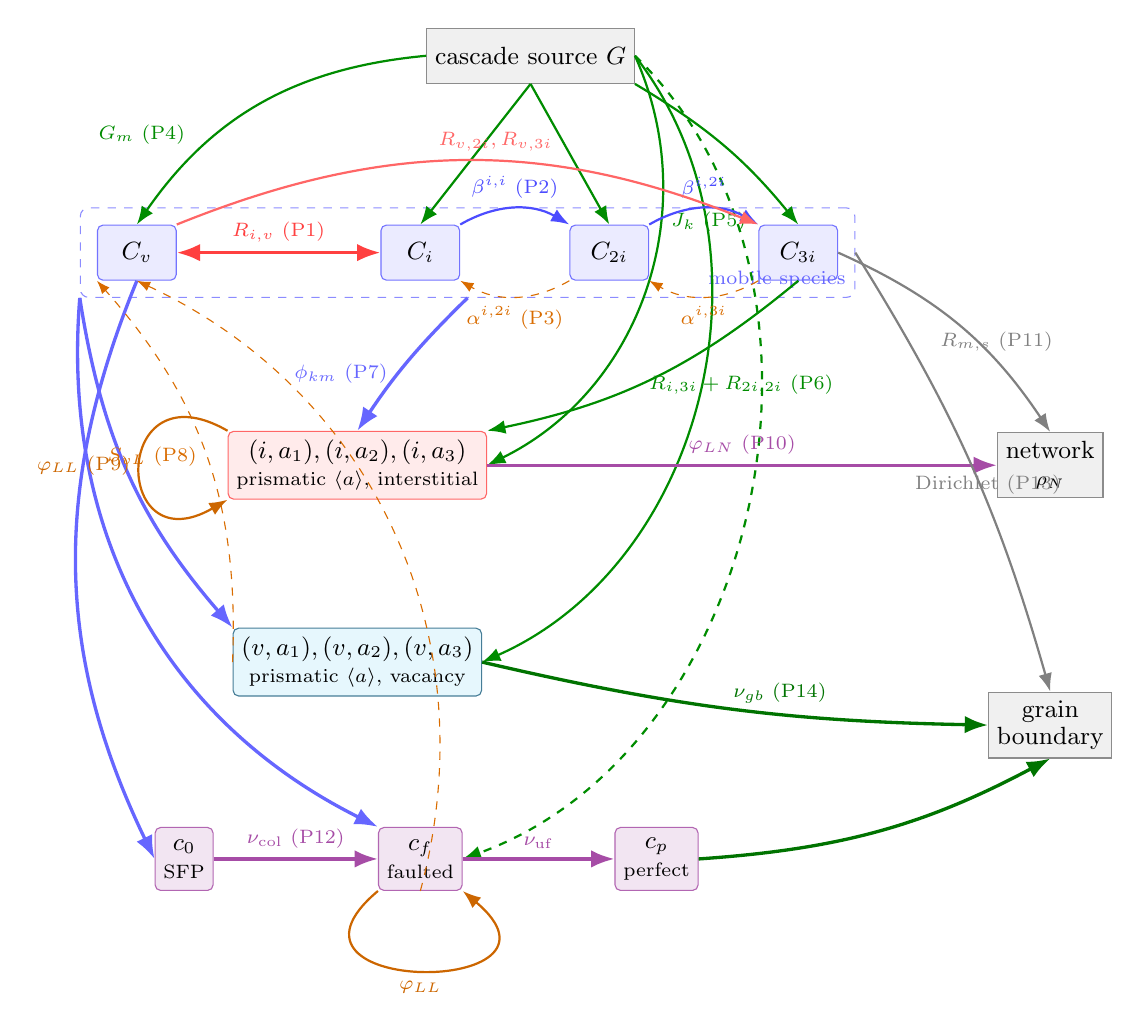
\begin{tikzpicture}[
  font=\small, >=Latex,
  mob/.style={draw, rounded corners=2pt, minimum height=7mm,
              minimum width=10mm, fill=blue!8, draw=blue!55},
  ipop/.style={draw, rounded corners=2pt, align=center, fill=red!8,
               draw=red!60, minimum height=8mm, inner sep=3pt},
  vpop/.style={draw, rounded corners=2pt, align=center, fill=cyan!10,
               draw=cyan!55!black, minimum height=8mm, inner sep=3pt},
  bpop/.style={draw, rounded corners=2pt, align=center, fill=violet!10,
               draw=violet!60, minimum height=8mm, inner sep=3pt},
  ext/.style={draw, align=center, fill=black!6, draw=black!45,
              minimum height=7mm, inner sep=3pt},
  clus/.style={->, thick, blue!70},
  capture/.style={->, very thick, blue!60},
  diss/.style={->, dashed, orange!85!black},
  rec/.style={<->, very thick, red!75},
  coal/.style={->, thick, orange!80!black},
  chain/.style={->, very thick, violet!70},
  snk/.style={->, thick, black!50},
  gbl/.style={->, very thick, green!45!black},
  src/.style={->, thick, green!55!black}]

  % ---- cascade source ---------------------------------------------------
  \node[ext] (G) at (-1.2,5.5) {cascade source $G$};

  % ---- the mobile block -------------------------------------------------
  \node[mob] (Cv)  at (-6.2,3.0) {$C_v$};
  \node[mob] (Ci)  at (-2.6,3.0) {$C_i$};
  \node[mob] (C2i) at (-0.2,3.0) {$C_{2i}$};
  \node[mob] (C3i) at ( 2.2,3.0) {$C_{3i}$};
  \node[draw, rounded corners=3pt, dashed, draw=blue!45, inner sep=6pt,
        fit=(Cv)(Ci)(C2i)(C3i), label={[font=\scriptsize, text=blue!60,
        anchor=south east]south east:{mobile species}}] (MOB) {};

  % ---- immobile families ------------------------------------------------
  \node[ipop] (ai) at (-3.4,0.3)
       {$(i,a_1),(i,a_2),(i,a_3)$\\[-1pt]
        \scriptsize prismatic $\langle a\rangle$, interstitial};
  \node[vpop] (av) at (-3.4,-2.2)
       {$(v,a_1),(v,a_2),(v,a_3)$\\[-1pt]
        \scriptsize prismatic $\langle a\rangle$, vacancy};
  \node[bpop] (c0) at (-5.6,-4.7) {$c_0$\\[-1pt]\scriptsize SFP};
  \node[bpop] (cf) at (-2.6,-4.7) {$c_f$\\[-1pt]\scriptsize faulted};
  \node[bpop] (cp) at ( 0.4,-4.7) {$c_p$\\[-1pt]\scriptsize perfect};

  % ---- external reservoirs ----------------------------------------------
  \node[ext] (NET) at (5.4,0.3)  {network\\[-1pt]\scriptsize $\rho_N$};
  \node[ext] (GB)  at (5.4,-3.0) {grain\\[-1pt]boundary};

  % ---- P4/P5 cascade sources --------------------------------------------
  \draw[src] (G.west) to[bend right=25]
       node[above left, pos=0.75, font=\scriptsize] {$G_m$ (P4)} (Cv.north);
  \draw[src] (G.south) -- node[right, pos=0.6, font=\scriptsize] {} (Ci.north);
  \draw[src] (G.south) -- (C2i.north);
  \draw[src] (G.south east) to[bend left=10] (C3i.north);
  \draw[src] (G.east) to[bend left=44]
       node[right, pos=0.35, font=\scriptsize] {$J_k$ (P5)} (ai.east);
  \draw[src] (G.east) to[bend left=52] (av.east);
  \draw[src, dashed] (G.east) to[bend left=58] (cf.east);

  % ---- P2 clustering, P3 dissociation ------------------------------------
  \draw[clus] (Ci.north east) to[bend left=30]
       node[above, font=\scriptsize] {$\beta^{i,i}$ (P2)} (C2i.north west);
  \draw[clus] (C2i.north east) to[bend left=30]
       node[above, font=\scriptsize] {$\beta^{i,2i}$} (C3i.north west);
  \draw[diss] (C2i.south west) to[bend left=30]
       node[below, font=\scriptsize] {$\alpha^{i,2i}$ (P3)} (Ci.south east);
  \draw[diss] (C3i.south west) to[bend left=30]
       node[below, font=\scriptsize] {$\alpha^{i,3i}$} (C2i.south east);

  % ---- P1 recombination and vacancy capture by clusters ------------------
  \draw[rec] (Cv) -- node[above, font=\scriptsize] {$R_{i,v}$ (P1)} (Ci);
  \draw[->, thick, red!60] (Cv.north east) to[bend left=22]
       node[above, pos=0.55, font=\scriptsize] {$R_{v,2i},R_{v,3i}$} (C3i.north west);

  % ---- P6 homogeneous loop nucleation -------------------------------------
  \draw[src, thick] (C3i.south) to[bend left=14]
       node[right, pos=0.55, font=\scriptsize]
       {$R_{i,3i}+R_{2i,2i}$ (P6)} (ai.north east);

  % ---- P7 capture at a loop or the SFP ------------------------------------
  \draw[capture] (MOB.south) to[bend right=6]
       node[left, pos=0.6, font=\scriptsize] {$\phi_{km}$ (P7)} (ai.north);
  \draw[capture] (MOB.south west) to[bend right=16] (av.north west);
  \draw[capture] (MOB.south west) to[bend right=34] (cf.north west);
  \draw[capture] (Cv.south) to[bend right=24] (c0.west);

  % ---- P8 peripheral emission ---------------------------------------------
  \draw[diss] (av.west) to[bend right=22]
       node[left, pos=0.5, font=\scriptsize] {$S_{vL}$ (P8)} (Cv.south west);
  \draw[diss] (cf.south) to[bend right=40] (Cv.south);

  % ---- P9 loop-loop coalescence -------------------------------------------
  \draw[coal] (ai.north west) to[out=150, in=210, looseness=5]
       node[left, font=\scriptsize] {$\varphi_{LL}$ (P9)} (ai.south west);
  \draw[coal] (cf.south west) to[out=-140, in=-40, looseness=5]
       node[below, font=\scriptsize] {$\varphi_{LL}$} (cf.south east);

  % ---- P10 loop-network, P11 mobile-network -------------------------------
  \draw[chain] (ai.east) -- node[above, font=\scriptsize]
       {$\varphi_{LN}$ (P10)} (NET.west);
  \draw[snk] (C3i.east) to[bend left=16]
       node[above, pos=0.7, font=\scriptsize] {$R_{m,s}$ (P11)} (NET.north);

  % ---- P12 basal chain ----------------------------------------------------
  \draw[chain] (c0) -- node[above, font=\scriptsize]
       {$\nu_{\mathrm{col}}$ (P12)} (cf);
  \draw[chain] (cf) -- node[above, font=\scriptsize]
       {$\nu_{\mathrm{uf}}$} (cp);

  % ---- P13 Dirichlet, P14 size-gated loop absorption ----------------------
  \draw[snk] (MOB.east) to[bend left=8]
       node[above, pos=0.6, font=\scriptsize] {Dirichlet (P13)} (GB.north);
  \draw[gbl] (av.east) to[bend right=6]
       node[above, pos=0.6, font=\scriptsize] {$\nu_{gb}$ (P14)} (GB.west);
  \draw[gbl] (cp.east) to[bend right=12] (GB.south);
\end{tikzpicture}
\caption{Reaction admissibility graph for the nine families of
\cref{eq:families}, with every edge class of \cref{tab:rag-processes}. The four
mobile species are boxed together because capture onto a loop sums over all of
them (\cref{eq:growth}), with a sign set by whether the species' polarity
matches the family's, so one bundled arrow per family is faithful where four
would be unreadable. Cascade production (green) feeds all four mobile species
and, as a separate partition of the same displacement rate, nucleates the
prismatic loops of both characters and the basal family directly; the dashed
source onto $c_f$ becomes a source onto $c_0$ instead when the basal chain is
active, which it is not in \cref{sec:results}. The interstitial prismatic
family has a second, homogeneous nucleation channel (P6) fed by
$2i+2i$ and $i+3i$ reactions among the mobile clusters, which is why the
mobile ladder and the loop populations are not separable. Dashed orange edges
run backwards from a population to the mobile pool: dissociation of a small
cluster (P3) and peripheral emission from a vacancy loop (P8). The three
prismatic variants of each character are drawn as one vertex for legibility;
they are separate populations that exchange nothing with one another and differ
only in habit normal, and the pyramid $c_0$ is not a loop --- it has no Burgers
vector, no perimeter and no coalescence channel, and enters only through a
capture cross-section.}
\label{fig:rag}
\end{figure}


\section{Cluster Dynamics Formulation}\label{sec:formulation}

\subsection{From the master equation to the reduced system}
\label{sec:master}

The general cluster-dynamics master equation for a population indexed by a
species label $\alpha$ and a size $n$ is a balance of gains and losses over the
edges of the graph of \cref{fig:rag},
\begin{equation}
  \frac{\partial C^\alpha_n}{\partial t}
  = -\nabla\!\cdot\!\bm J^\alpha_n
    + G^\alpha_n
    + \sum_{\beta,n'} \bigl[\mathcal K^{\alpha\beta}_{n-n',n'}C^\beta_{n-n'}C^{\beta'}_{n'}
      - \mathcal K^{\alpha\beta}_{n,n'}C^\alpha_nC^\beta_{n'}\bigr]
    + \varepsilon^\alpha_{n+1}C^\alpha_{n+1} - \varepsilon^\alpha_nC^\alpha_n
    - \mathcal D^\alpha_n C^\alpha_n ,
  \label{eq:master}
\end{equation}
with $\bm J^\alpha_n=-\bm D^\alpha_n\nabla C^\alpha_n$ the diffusive flux,
$G^\alpha_n$ the cascade source, $\mathcal K$ the pairwise reaction kernels,
$\varepsilon$ the thermal emission rates, and $\mathcal D$ the absorption rate
at fixed sinks. \Cref{eq:master} is one equation per $(\alpha,n)$ and per mesh
node, and is not solvable as written for the size ranges of interest.

Two reductions bring it to the system integrated here, and they cut in different
directions.

\paragraph{Mobile species: truncate the ladder.} Only the monomers and the
smallest interstitial clusters migrate. The mobile set is closed at
$\spvec{m}_M=[-1,+1,+2,+3]^{T}$ --- monovacancy, mono-, di- and tri-interstitial
--- with the signed entries $m^k$ carrying the polarity
$p^k=m^k/|m^k|$. Everything larger is immobile and is carried by the second
reduction. The mobile block retains its spatial derivative, because transport is
what it is for.

\paragraph{Immobile families: truncate the moments, keep the variants.} For the
immobile families the ladder in $n$ is replaced by the first three moments of
the size distribution of each family in \cref{eq:families},
\begin{equation}
  n^k_{sL}=\!\int\! f_k\,\mathrm{d}m,
  \qquad
  c^k_{sL}=\!\int\! m f_k\,\mathrm{d}m,
  \qquad
  q^k_{sL}=\!\int\! m^2 f_k\,\mathrm{d}m,
  \label{eq:moments-def}
\end{equation}
closed by the log-normal ansatz of \cref{sec:moments}. The immobile block loses
its spatial derivative entirely: a loop does not diffuse, and the only thing
that couples one node's loops to another's is the mobile field. That is not an
approximation --- it is the property that makes the numerical method of
\cref{sec:split} possible.

\subsection{The mobile block}
\label{sec:mobile}

Because the mobile species reach quasi-steady state on a time scale
$\tau_M\sim(k^2D)^{-1}$ of order microseconds, while the immobile families evolve
on the dose scale ($1\,\mathrm{dpa}=10^{7}\,\mathrm{s}$ at
$G=10^{-7}\,\mathrm{dpa\,s^{-1}}$), the mobile block is solved as a
\emph{steady} reaction--diffusion problem for the immobile state currently held.
Writing $\spvec c_M=[c^v,c^i,c^{2i},c^{3i}]^{T}$ in per-atom units,
\begin{equation}
  \spvec 0 = -\nabla\!\cdot\!\spvec J
    + \spvec P_M
    + \tfrac12\,(\spmat I\otimes\spvec c_M^{T})\,\spmat R_2\,\spvec c_M
    + (\spmat E-\spmat D)\,\spvec c_M
    + \spvec S_{vL},
  \label{eq:master-c}
\end{equation}
where upright sans-serif bold denotes arrays in \emph{species space} and
bold italic ordinary Cartesian vectors and tensors, so that the entries
$\bm J^{x}=-\bm D^{x}\nabla c^{x}$ of the stacked flux $\spvec J$ are themselves
Cartesian vectors and $\nabla\cdot$ acts on each.

The terms are, in order: the cascade production
$\spvec P_M=G\varepsilon\spvec f$, with $G$ the displacement rate, $\varepsilon$
the surviving efficiency and $\spvec f$ the partition of production among the
mobile species; the second-order reactions $\spmat R_2$, whose entries are the
pairwise rate constants
\begin{equation}
  \beta^{m,n}=\frac{A^{m,n}}{\Omega}\,(\overline D^{m}+\overline D^{n})(r^{m}+r^{n}),
  \qquad
  r^{m}=\begin{cases}
    \left(\dfrac{3\Omega}{4\pi}\right)^{1/3}, & |m^{m}|=1,\\[9pt]
    \left(\dfrac{|m^{m}|\,\Omega}{\pi b}\right)^{1/2}, & |m^{m}|>1,
  \end{cases}
  \label{eq:rates}
\end{equation}
with the recombination-volume factor $\beta_r$ carried on the
interstitial--vacancy channel and the combinatorial factors retained on the
like-species channels; the thermal emission matrix $\spmat E$, whose entries are
$\alpha^{m,n}=\beta^{m,n}\exp(-E^{b}_{m,n}/k_BT)$; the linear absorption matrix
$\spmat D$; and $\spvec S_{vL}$, the vacancies returned to the pool by
peripheral emission from vacancy loops (\cref{app:emission}).

The absorption matrix is where the immobile population acts back on the mobile
one, and it is written so that no defect can be counted twice:
\begin{equation}
  \spmat D = \mathrm{diag}\{\spvec\omega\odot\spvec C_s\}
             + \spmat D_d\,\spmat K_{\mathcal L},
  \qquad
  \spmat D_d=\mathrm{diag}\{\overline D^{v},\overline D^{i},
                            \overline D^{2i},\overline D^{3i}\},
  \label{eq:KM}
\end{equation}
whose first term carries the \emph{network alone},
\begin{equation}
  C_s^{v}=\frac{a^2}{z_c}\rho_N,
  \qquad
  C_s^{i}=\frac{a^2}{z_c}Z_N\rho_N,
  \label{eq:sinkconc}
\end{equation}
and whose second carries the loops through the diagonal sink-strength block
\begin{equation}
  \spmat K_{\mathcal L}=\mathrm{diag}\{\spvec k^{2}\},
  \qquad
  k_m^{2}=\sum_{(s,k)\in\mathcal F_L}\! Z_{sk,m}\,\rho^k_{sL}
        \;+\;Z_{vc_0,m}\,\alpha_{\mathrm{sfp}}\,\pi R^{c_0}_{vL}\,
             \frac{n^{c_0}_{vL}}{\Omega}
        \;+\;Z_{N,m}\,\rho_N .
  \label{eq:KL}
\end{equation}
The loops must not also appear in \cref{eq:sinkconc}, or their absorption would
be counted once as a network sink and once as loop growth. The middle term of
\cref{eq:KL} is the stacking-fault pyramid, which has no line density and enters
through a compact capture cross-section instead; \cref{eq:Pi-identity} below
shows that a cross-section is the only thing either side ever asks of a family.

\paragraph{Boundary conditions.} On a free surface or a grain boundary the
mobile species are pinned at thermal equilibrium,
\begin{equation}
  c^{v}=c^{v,\mathrm{eq}}=\exp(-E^{f}_v/k_BT),
  \qquad
  c^{i}=c^{2i}=c^{3i}=0 \quad\text{on }\partial\Omega_D,
  \label{eq:bc}
\end{equation}
which is process class P13 of \cref{tab:rag-processes}. This replaces the
mean-field grain-boundary sink strength $k^2_{gb}\simeq6\sqrt{k^2}/d$ by a
boundary condition, and the depleted layer in front of it becomes an output
rather than a parameter. Faces declared periodic instead carry periodic
conditions on all four species.

\subsection{Anisotropic transport and the single anisotropy parameter}
\label{sec:transport}

Each mobile species carries a diffusion tensor
$D^{x}_{ij}=D^{x}_{0ij}\exp(-E^{xm}_{ij}/k_BT)$, diagonal in the crystal frame
with the basal components equal and the $c$-axis component distinct. The whole
of that anisotropy is expressed by one number per species,
\begin{equation}
  p^{m}=\left(\frac{D^{m}_{\parallel}}{D^{m}_{\mathrm{basal}}}\right)^{1/6},
  \label{eq:pm}
\end{equation}
and the migration energies are generated from it at \emph{fixed} effective
diffusivity,
\begin{equation}
  E^{m}_{\langle11\rangle}=E^{m}_{\langle22\rangle}=E^{m}_{\mathrm{eff}}+2k_BT\ln p^{m},
  \qquad
  E^{m}_{\langle33\rangle}=E^{m}_{\mathrm{eff}}-4k_BT\ln p^{m},
  \label{eq:Emsplit}
\end{equation}
so that the orientation-averaged diffusivity
$\overline D^{m}=(\det\bm D^{m})^{1/3}$ is exactly the scalar $D_m$ of the
mean-field kinetics. \textbf{No mobility is redefined by the anisotropy --- only
its directional weighting.} This is the technical device that makes the
formulation self-consistent: \cref{eq:pm,eq:Emsplit} are a change of variable in
which $p^{m}$ is the only anisotropy the model has, and \cref{sec:efficiencies}
uses that same $p^{m}$ and no other parameter.

\subsection{Capture efficiencies}
\label{sec:efficiencies}

Every capture efficiency is a product of factors, one per degeneracy to be
broken:
\begin{equation}
  Z_{sk,m}(\bm\sigma)
  = \underbrace{Z^{0}_m}_{\text{elastic bias}}\;
    \underbrace{A_{h(k)}(p^{m})}_{\text{DAD, orientation}}\;
    \underbrace{X_{s,m}}_{\text{character}}\;
    \underbrace{\left[1+\frac{\Delta Z^{\mathrm{SIPA}}_{h(k),m}(\sigma_{kk})}
                            {Z^{0}_mA_{h(k)}(p^{m})}\right]}_{\text{stress, SIPA}},
  \label{eq:Zsk}
\end{equation}
with $h(k)\in\{a,c\}$ the habit of family $k$ and the Woo diffusional-anisotropy
factors~\citep{woo1988theory,woo1981sink,po2026tensorialdad}
\begin{equation}
  A_a(p)=\frac{p+p^{-2}}{2},
  \qquad
  A_c(p)=p .
  \label{eq:Afactors}
\end{equation}
Each factor breaks exactly one degeneracy and is silent on the others.
$A_{h(k)}$ depends on the habit alone --- on the angle between the loop normal
and the $c$ axis --- and therefore assigns one value to all six prismatic
families and one to all three basal states, the pyramid included, whose base is
$(0001)$ so that $h(c_0)=c$. It separates prismatic from basal but is degenerate
in character. $X_{s,m}$ is the character factor, which separates an interstitial
from a vacancy loop of the same habit~\citep{marchrico2023,marchrico2025}; the
coexistence window it opens has log-width $\ln\chi$ with
$\chi=X_{iI}X_{vV}/(X_{iV}X_{vI})$.

\textbf{\Cref{eq:Zsk} contains no free bias.} $A_{h(k)}$ is built from the same
$p^{m}$ that \cref{eq:Emsplit} puts into the diffusion tensors, so a change in
the transport anisotropy moves the growth laws and the sink strengths of
\cref{eq:KL} together. The two remaining constants, $Z^{0}_m$ and $X_{s,m}$, are
calibrated (\cref{sec:calibration}); the orientation dependence is not.

The forms in \cref{eq:Afactors} are not monotone in the same way, and the
consequence is quantitative and easily missed. $A_c(p)=p$ increases without
bound, while $A_a(p)=(p+p^{-2})/2$ has its minimum at $p=2^{1/3}=1.2599$. A
single change of $p^{v}$ therefore pushes the basal and prismatic families in
\emph{opposite} directions, starving \cloop{} growth while accelerating \aloop{}
shrinkage, or the reverse. Any statement about the effect of anisotropy that
does not distinguish the two habits is incomplete.

\subsection{Conditions for the growth of every variant}
\label{sec:coexistence}

The experimental record poses a problem that a mean-field model does not
automatically solve, and the analysis that follows is what forces the
formulation to be self-consistent in the sense of
\cref{sec:intro}(a). It is also the analysis that decides which
of the nine families grow, at what mobile fluxes, and under what conditions two
of them can grow at once.

\subsubsection{The growth conditions}
\label{sec:growconds}

Define the mobile flux aggregates and their ratio,
\begin{equation}
  \Phi_I=\sum_{n\in I_{\mathrm{mob}}}n\,\overline D^{I_n}c^{I_n},
  \qquad
  \Phi_V=\overline D^{v}c^{v},
  \qquad
  x\equiv\frac{\Phi_V}{\Phi_I},
  \label{eq:fluxscales}
\end{equation}
which reduce to $\Phi_I=\overline D^{i}c^{i}$ and
$\Phi_V=\overline D^{v}c^{v}$ in the monomer approximation. With $Z_{s,m}$ the
capture efficiency of family $s$ for mobile species $m$, the net driving force
on a family of character sign $\eta_s=\pm1$ is
\begin{equation}
  F_s=\eta_s\left(Z_{s,I}\Phi_I-Z_{s,V}\Phi_V\right),
  \label{eq:Fsigma}
\end{equation}
so that each family grows or shrinks according to which side of its own
threshold the ratio $x$ falls on:
\begin{equation}
  \text{interstitial family }s\text{ grows}\iff x<\frac{Z_{s,I}}{Z_{s,V}},
  \qquad
  \text{vacancy family }s\text{ grows}\iff x>\frac{Z_{s,I}}{Z_{s,V}} .
  \label{eq:growconds}
\end{equation}

\Cref{eq:growconds} is the whole of the growth problem, and it says something
uncomfortable. Every family reduces to \emph{one} threshold, the ratio of its
own two efficiencies, and $x$ is a single number. Under identical local fluxes
and identical capture coefficients an interstitial and a vacancy loop of the
same orientation therefore \emph{cannot} both grow: whichever side of the shared
threshold $x$ lies on, one of them is shrinking. Yet both prismatic characters
are observed together in irradiated
Zr~\citep{jostsons1977nature,griffiths1988review,carpenter1981study,%
marchrico2025}. Coexistence is thus a statement that at least one idealization
has failed --- homogeneity, identical capture coefficients, identical nucleation
pathways, identical variants, or identical irradiation history --- and the
remainder of this subsection identifies which, and what each candidate can and
cannot deliver.

\subsubsection{What diffusional anisotropy does, and where it stops}
\label{sec:dad-window}

With the diffusion tensors and the orientation factors of
\cref{eq:pm,eq:Afactors}, the prismatic and basal thresholds separate:
\begin{equation}
  x_a=\frac{Z^{0}_{I}A_a(p^{i})}{Z^{0}_{V}A_a(p^{v})},
  \qquad
  x_c=\frac{Z^{0}_{I}A_c(p^{i})}{Z^{0}_{V}A_c(p^{v})},
  \label{eq:thresholds}
\end{equation}
and because $A_a(p)=(p+p^{-2})/2$ exceeds $A_c(p)=p$ for $p<1$ while the two
coincide at $p=1$, the ordering $x_c<x_a$ holds whenever $p^{i}<p^{v}$.
Prismatic interstitial and basal vacancy loops then grow \emph{together}
throughout
\begin{equation}
  \boxed{\;x_c<x<x_a\;},
  \qquad
  \ln\frac{x_a}{x_c}=\ln\frac{g(p^{v})}{g(p^{i})},
  \qquad
  g(p)\equiv\frac{2}{1+p^{-3}},
  \label{eq:window}
\end{equation}
with $g$ strictly increasing, so the window is open exactly when $p^{i}<p^{v}$
and closes as $p^{i}\to p^{v}$. In the near-isotropic-vacancy limit
$p^{v}\simeq1$ the width reduces to the familiar form
$x_a-x_c=(Z^{0}_{I}/Z^{0}_{V})(1-(p^{i})^{3})/2(p^{i})^{2}$. At
$200\,^{\circ}$C, with $Z^{0}_{I}/Z^{0}_{V}\approx1.05$--$1.15$ and
$p^{i}\approx0.89$--$0.92$~\citep{woo1988theory,christien2009cluster,%
barashev2015theoretical,li2020coupled}, the window is open but narrow:
$x_c\approx1.0<x<x_a\approx1.2$.

Three things are worth separating here, because they are routinely conflated.

\textbf{The elastic bias opens nothing.} $Z^{0}_{I}/Z^{0}_{V}>1$ multiplies
\emph{both} thresholds in \cref{eq:thresholds} and so shifts them together; it
cancels from the width in \cref{eq:window} entirely. It does narrow the
prismatic-interstitial/basal-vacancy window in a practical sense, by pushing
$x_c$ toward unity, but it cannot create an interval where none exists.

\textbf{What positions $x$ inside the window is the production bias.} The
excess of freely migrating vacancies left when more of the interstitial yield is
locked into in-cascade clusters, $\eta=\varepsilon_V/\varepsilon_I\gtrsim1$,
sets where in $(x_c,x_a)$ the operating point sits; a $0$--$20\%$ excess
suffices. \textbf{Neither substitutes for the other.} DAD opens the interval and
the production bias places the point inside it: at $p^{i}=p^{v}$ the thresholds
coincide and no value of $\eta$ can satisfy both conditions at once, while with
the window open but $\eta$ badly placed the model simply grows one family and
dissolves the other.

\textbf{DAD is degenerate in character, and that is where it stops.}
\Cref{eq:Zsk} assigns one orientation factor $A_{h(k)}(p^{m})$ to every family
sharing a habit, so the interstitial and the vacancy prismatic variants receive
the \emph{same} pair of efficiencies and hence the same threshold,
\begin{equation}
  \frac{Z_{a_k I,I}}{Z_{a_k I,V}}
  \;\xrightarrow[\ \text{DAD alone}\ ]{}\;
  \frac{Z_{a_k V,I}}{Z_{a_k V,V}} .
  \label{eq:dad-degenerate}
\end{equation}
The prismatic window closes identically, and DAD is silent on the coexistence of
interstitial and vacancy \aloop{} loops on one habit --- which is the
coexistence the experiments report. Two mechanisms remove that degeneracy, and
the formulation carries both.

\subsubsection{Resolution 1: the flux ratio is a field}
\label{sec:resolution-field}

Promote $x$ to $x(\xv,t)=\Phi_V(\xv,t)/\Phi_I(\xv,t)$. Because interstitials
migrate far faster than vacancies, the interstitial channel responds first and
most sharply to any transient or gradient.

In \emph{time}, the nucleation transient --- which in Zr extends over of order
$1\,$dpa --- is strongly interstitial-rich, so $x(t)\ll x_c$ and interstitial
loops grow while vacancy loops merely nucleate and sit sub-critical; as the
vacancy supersaturation builds, $x(t)$ rises into $(x_c,x_a)$ and the vacancy
families begin to grow, with the interstitial loops established earlier
persisting alongside them.

In \emph{space}, sinks --- grain boundaries, free surfaces, precipitates, the
network --- make the mobile fields non-uniform, and because the interstitial
diffusion length far exceeds the vacancy one, interstitials drain into the far
field while vacancies pile up locally, so $x(\xv)$ is depressed far from sinks
and enhanced near them. A single specimen then contains regions on both sides of
the prismatic threshold. \Cref{sec:results-mobile} measures exactly this
structure: boundary layers of $8$--$46\,$nm that differ by species, so $x$
varies systematically across them.

\textbf{This mechanism costs nothing to include: a spatially resolved
formulation carries $x(\xv,t)$ natively and does not have to be told to.} Its
limitation is equally plain. It leaves $Z_{a_kI,\cdot}=Z_{a_kV,\cdot}$ intact
and buys coexistence by declining to evaluate the two growth conditions at the
same point of space and time, so it predicts \emph{segregated} coexistence and
cannot give locally simultaneous growth in a homogeneous volume.

\subsubsection{Resolution 2: capture is character-resolved}
\label{sec:resolution-character}

March-Rico, Blondel and Wirth~\citep{marchrico2025} compute the defect--loop
interaction energy atomistically and replace geometric intersection by a
drift--diffusion capture,
\begin{equation}
  \bm J_\alpha=-\bm D_\alpha\left[\nabla c^{\alpha}
    +\frac{c^{\alpha}}{k_BT}\nabla E^{\alpha L}_{\mathrm{int}}\right],
  \qquad \alpha=i,v,
  \label{eq:drift-diffusion}
\end{equation}
which reduces in the rate equations to effective capture radii entering
additively in the reaction volume. \emph{Spontaneous} capture radii are nearly
the same for all loops and enlarge every reaction volume without separating
characters; \emph{thermal-drift} radii do separate them, because the dilatational
field of an interstitial loop attracts interstitials over a longer range than it
attracts vacancies, and conversely for a vacancy loop. The result is a
\textbf{same-type capture bias}, carried in \cref{eq:Zsk} by the factor
$X_{s,m}$. Defining the character-splitting factor
\begin{equation}
  \chi\equiv
  \frac{Z_{a_kI,I}/Z_{a_kI,V}}{Z_{a_kV,I}/Z_{a_kV,V}}
  =\frac{X_{iI}X_{vV}}{X_{iV}X_{vI}},
  \label{eq:chi}
\end{equation}
the prismatic window $Z_{a_kV,I}/Z_{a_kV,V}<x<Z_{a_kI,I}/Z_{a_kI,V}$ is
non-empty if and only if $\chi>1$, with logarithmic width $\ln\chi$.

\Cref{eq:chi} is the exact character analogue of the orientation width
\cref{eq:window}: $\ln(x_a/x_c)$ measures how far diffusional anisotropy
separates prismatic from basal, and $\ln\chi$ how far thermal-drift capture
separates interstitial from vacancy \emph{within} one prismatic habit. Because
$\chi>1$ opens a genuine interval, a single uniform steady $x$ satisfies both
conditions at once --- which is the stronger claim, and the more falsifiable
one.

\subsubsection{Two ingredients that are not optional}
\label{sec:not-optional}

\textbf{In-cascade vacancy clustering supplies the embryos.} Without them the
capture bias has nothing to act on: homogeneous nucleation of a vacancy loop
against the prevailing interstitial bias is prohibitively slow. It is the
\emph{same} clustering asymmetry that generates the production bias $\eta$, so
the two must not be fitted as independent inputs.

\textbf{Cascade overlap reduces the effective generation rate with dose,}
$\tilde g(\gamma)=\varepsilon(\gamma)g$, saturating over $0.01$--$0.1\,$dpa to a
small residual fraction. This is what lets coarsening rather than unbounded
nucleation dominate at high dose. Applied as a single scalar to both species it
rescales dose without moving $x$: it is a rate effect, not a threshold effect.

\Cref{tab:mechanisms} summarizes the division of labor.

\begin{table}[htbp]
\caption{What each ingredient does to the growth criterion \cref{eq:growconds}.
Only the last two separate loops of the same prismatic orientation; only
character-resolved capture does so locally and instantaneously.}
\label{tab:mechanisms}
\centering\small
\begin{tabularx}{\textwidth}{@{}>{\raggedright\arraybackslash}p{0.20\textwidth}
                              >{\raggedright\arraybackslash}p{0.20\textwidth}X@{}}
\toprule
Ingredient & Acts on & What it does, and does not do \\
\midrule
Elastic bias $Z^{0}_{I}/Z^{0}_{V}$ & both thresholds together &
  Shifts $x_a$ and $x_c$ jointly; opens no window, and narrows the
  prismatic-interstitial/basal-vacancy window by pushing $x_c$ toward unity. \\
\addlinespace
Diffusional anisotropy, $p^{i}<p^{v}$ & orientation &
  Opens the prismatic-interstitial/basal-vacancy window of width
  \cref{eq:window}. Cannot separate loops of one orientation,
  \cref{eq:dad-degenerate}. \\
\addlinespace
Production bias $\eta$ & position of $x$ &
  Places $x$ inside whatever window exists. Creates no window; with $x_a=x_c$ it
  merely switches which family grows. \\
\addlinespace
Flux field $x(\xv,t)$ & position of $x$, resolved in space and time &
  Lets the two prismatic conditions be met at different doses or different
  places. Predicts \emph{segregated} coexistence. Native to a spatially
  resolved model. \\
\addlinespace
Thermal-drift capture, $\chi>1$ & character &
  Opens the prismatic window of logarithmic width $\ln\chi$; gives \emph{local}
  simultaneous growth. Needs in-cascade clustering for the embryos, and still
  needs $x$ positioned inside. \\
\bottomrule
\end{tabularx}
\end{table}

\subsubsection{Why this forces the formulation}
\label{sec:forces-formulation}

Three requirements follow, and together they are the content of
\cref{sec:classes,sec:formulation}.

\begin{enumerate}[itemsep=3pt]
\item \textbf{The immobile families must be crystallographic.} A scalar
      aligned/non-aligned split can express \emph{how much} of a population a
      stress favors but not \emph{which} prismatic system it favors, and it has
      no meaning at all under a multiaxial stress or a stress field. Resolving
      $a_1,a_2,a_3$ makes the resolved stress on each habit a computed
      quantity, and carrying both characters on each variant is what makes
      \cref{eq:chi} representable at all. Splitting the basal population into a
      faulted and a perfect state is forced separately, by the fact that the two
      store different vacancy content per unit area (\cref{tab:cd-families}).
\item \textbf{The capture efficiencies must come from the transport tensors.}
      This is sense~(a) of \cref{sec:intro}, and
      \cref{eq:window} is why it matters rather than merely being tidy: the
      width of the co-growth window is a function of the transport anisotropy
      \emph{alone}. A model that diffuses with one anisotropy and biases its
      sinks with an independent phenomenological pair
      $(\delta_i,\delta_v)$ can therefore report a window that its own transport
      does not support. The phenomenological pair remains recoverable as the
      exact map
      \begin{equation}
        \delta_m=\frac{A_a(p^{m})-A_c(p^{m})}{A_a(p^{m})+A_c(p^{m})}
                =\frac{1-(p^{m})^{3}}{1+3(p^{m})^{3}},
        \label{eq:deltamap}
      \end{equation}
      which gives $\delta_i\approx0.07$--$0.09$ and $\delta_v\approx0$ at the
      $200\,^{\circ}$C anisotropies above. Note that $Z^{0}_{I}/Z^{0}_{V}$ does
      not appear in $\delta_m$ and must be carried separately, which is why
      \cref{eq:Zsk} is the more faithful input.
\item \textbf{The mobile field must be spatially resolved.}
      \Cref{sec:resolution-field} is not available to a $0$-D model. It requires
      $x(\xv,t)$, hence the reaction--diffusion problem of \cref{eq:master-c}
      with real boundary conditions --- and it is one of the two independent
      reasons for the spatial treatment, the other being that surfaces and grain
      boundaries are the dominant defect sink in any specimen small enough to be
      examined (\cref{tab:conservation}).
\end{enumerate}

\paragraph{Two cautions, so that neither is later mistaken for a prediction.}
The thermal-drift radii behind \cref{eq:chi} scale as $(T_m/T)^{m_d}$ with
$T_m=2128\,$K, so with $m_d>0$ the same-type bias, and hence $\chi$, is
\emph{strongest at low temperature} --- while the observed vacancy \aloop{}
fraction \emph{increases} with temperature. These are not contradictory: the
temperature dependence of the vacancy fraction is controlled largely by
nucleation, by vacancy mobility, and by thermal emission from small vacancy
clusters, none of which is contained in $\chi$. But reproducing the measured
vacancy fraction against temperature is a genuine test of the combined model
rather than something it obtains for free. The related hazard is double
counting: the same-type capture bias \emph{is} an elastic-interaction effect,
and so is the conventional dislocation bias $Z^{0}_{I}/Z^{0}_{V}>1$. Only one of
the two should carry the interstitial--vacancy asymmetry. In the calibration of
\cref{sec:calibration} the fitted $\chi=1$, so the asymmetry is carried by
$Z^{0}$ alone and the question does not arise --- which is also to say that the
present parameter set exercises Resolution~1 and not Resolution~2.

\subsection{The immobile block}
\label{sec:immobile}

\paragraph{Growth.} All nine families obey one growth law, in which the stored
content changes under the net biased flux of the correct sign:
\begin{equation}
  \left.\dot c^k_{sL}\right|_{\mathrm{growth}}
  = \Pi^k_{sL}\;\eta_s\!\!\sum_{m\in\{v,i,2i,3i\}}\!\!
    |m|\;\overline D^{m}\,Z_{sk,m}\,c^{m}\,\varsigma_s(m),
  \label{eq:growth}
\end{equation}
with $\varsigma_s(m)=+1$ when the polarity of species $m$ matches the character
$s$ and $-1$ otherwise. The geometric prefactor is
\begin{equation}
  \Pi^k_{sL}=\frac{\lambda_k}{\ell}\,\varsigma^{\mathrm{sink}}_k
             \sqrt{n^k_{sL}c^k_{sL}},
  \qquad
  \ell\equiv\frac{z_c\Omega}{2\pi a^{2}},
  \label{eq:loopprefactor}
\end{equation}
and because $\rho^k_{sL}=2\pi\lambda_k\sqrt{n^k_{sL}c^k_{sL}}$ by
\cref{eq:radius},
\begin{equation}
  \Pi^k_{sL}=\varsigma^{\mathrm{sink}}_k\,\frac{\rho^k_{sL}}{2\pi\ell}
  \qquad\text{identically, for every }(s,k)\in\mathcal F_L .
  \label{eq:Pi-identity}
\end{equation}
\emph{The prefactor in the growth law is the family's own sink density divided
by $2\pi\ell$.} That identity is what makes \cref{eq:growth} and \cref{eq:KL}
two readings of one quantity, and it is what carries the growth law onto the
pyramid unchanged: a family needs no geometry beyond the capture cross-section
it presents, and the pyramid supplies that cross-section as
$\Pi^{c_0}_{vL}=\varsigma^{\mathrm{sink}}_{c_0}\alpha_{\mathrm{sfp}}
R^{c_0}_{vL}n^{c_0}_{vL}/2\ell$.

\paragraph{Nucleation.} Cascade production deposits directly into the immobile
families at a rate $G_k=G\,\epsilon_k$ per family, each new cluster carrying
$m^{\mathrm{nuc}}_k$ defects, so that
$\dot n^k_{sL}|_{\mathrm{nuc}}=J^k_{sL}=G_k/m^{\mathrm{nuc}}_k$ and
$\dot c^k_{sL}|_{\mathrm{nuc}}=G_k$. The partition $\epsilon_k$ and the
nucleation sizes are calibrated quantities.

\paragraph{Coalescence.} Loops are removed by overlap with other loops and with
the network. With $N=n/\Omega$, $R=\lambda\sqrt{c/n}$, and the radii capped at
the relevant spacing ($R_{LL}=\min(R,(\Omega/n)^{1/3})$,
$R_{LN}=\min(R,\rho_N^{-1/2})$), the Avrami overlap probabilities and rate
scales are
\begin{align}
  \varphi_{LL}&=1-\exp\!\left(-\kappa_{LL}\tfrac43\pi R_{LL}^{3}N\right), &
  \varphi_{LN}&=1-\exp\!\left(-\kappa_{LN}\pi R_{LN}^{2}\rho_N\right),
  \nonumber\\
  \nu_{LL}&=c_{LL}\,v_{\mathrm{abs}}\,N^{1/3}, &
  \nu_{LN}&=c_{LN}\,v_{\mathrm{abs}}\,\sqrt{\rho_N},
  \label{eq:avrami}
\end{align}
giving the number and content losses
\begin{equation}
  \Delta N_{LN}=\nu_{LN}\varphi_{LN}n,
  \qquad
  \Delta N=\nu_{LL}\varphi_{LL}n+\Delta N_{LN},
  \qquad
  \Delta C=\nu_{LN}\varphi_{LN}c .
  \label{eq:coal}
\end{equation}
The like-loop channel merges two loops into a larger one and therefore
\emph{conserves content}, removing density only; the loop--network channel
removes both, and the removed content is booked as network sink absorption so
the point-defect balance stays closed. The rate scale is set by the
\emph{absorbed}-flux climb speed $v_{\mathrm{abs}}$ rather than the net growth
velocity, so coarsening persists at saturation. The capping is what makes
\cref{eq:avrami} saturate rather than diverge as the number density collapses,
and $\varphi_{LL}\to1$ is the model's own statement that its mean-field
treatment of coalescence has expired --- the detector used in
\cref{sec:coarsening}.

\paragraph{Emission.} Vacancy loops exchange vacancies across their own
perimeter at a rate set by a size-dependent binding energy computed from the
anisotropic loop self-energy (\cref{app:emission}), one expression serving both
characters, so that the same mechanism shrinks a vacancy loop and grows an
interstitial one and the classical climb threshold emerges rather than being
imposed. This channel replaces the two fitted annealing lifetimes of the
mean-field model. It returns vacancies to the mobile pool through $\spvec S_{vL}$
in \cref{eq:master-c}.

\paragraph{The basal chain.} The three basal states are linked by two one-way
activated transfers,
\begin{equation}
  c_0 \;\xrightarrow{\;\nu_{\mathrm{col}}\;}\; c_f
      \;\xrightarrow{\;\nu_{\mathrm{uf}}\;}\; c_p ,
  \label{eq:basal-chain}
\end{equation}
both size-gated, and both conserving vacancies exactly: the content leaving one
state enters the next, and only the \emph{number} changes, because the states
store different vacancy content per unit area
(\cref{tab:cd-families})~\citep{liu2020two,varvenne2014vacancy,marchrico2025}.
The chain is basal and has no prismatic counterpart: \emph{ab initio}-parameterized
formation energies place the prismatic vacancy \aloop{} loop \emph{below} both
the compact cavity and the faulted basal loop, so the planar prismatic loop is
already the ground-state geometry rather than something a compact cluster must
convert into~\citep{varvenne2014vacancy}. \textbf{None of the basal-chain rates
is calibrated}; the formulation gives their Arrhenius form and no measurement in
this work supplies the barriers, so the chain is switched off in the calculation
of \cref{sec:results} and its consequences are discussed in
\cref{sec:conclusions}.

\subsection{The size distribution and its closure}
\label{sec:moments}

Carrying only $n$ and $c$ assigns every loop at a point the same size, and the
population that produces is monodisperse by construction. The second content
$q^k_{sL}$ removes that restriction. Its Fokker--Planck part is
\begin{equation}
  \left.\dot q^k_{sL}\right|_{\mathrm{FP}}
  = 2\Pi^k_{sL}\Bigl[\;
      \underbrace{\Sigma^{\mathrm{net}}_k\,\bar m^k_{sL}\,\Delta_k^{3/8}}_{\text{drift}}
      \;+\;
      \underbrace{\tfrac12\,\Sigma^{\mathrm{gro}}_k\,\Delta_k^{-1/8}}_{\text{spreading}}
    \Bigr],
  \label{eq:q-FP}
\end{equation}
to which nucleation, the floor current and the basal transfers are appended
weighted by $m^{2}$ rather than $m^{1}$ or $m^{0}$:
\begin{equation}
  \dot q^k_{sL}=\left.\dot q^k_{sL}\right|_{\mathrm{FP}}
    + J^k_{sL}\bigl(m^{\mathrm{nuc}}_k\bigr)^{2}
    - m_{\min}^{2}\,\Phi^k_{\min}
    \;\pm\;\Gamma^{q}_{\theta}.
  \label{eq:qdot}
\end{equation}
The spreading term does not vanish when the family stops growing: at
$\Sigma^{\mathrm{net}}_k=0$ the drift term is zero and
$\dot q^k_{sL}=\Pi^k_{sL}\Sigma^{\mathrm{gro}}_k\Delta_k^{-1/8}>0$, so the
distribution keeps broadening at fixed mean size and fixed number. There is no
value of the two lower moments that expresses that, which is the argument for
carrying the third.

Closing \cref{eq:qdot} with a log-normal $f_k(m)$ determines its two parameters
from the three carried moments,
\begin{equation}
  \bar m^k_{sL}=\frac{c^k_{sL}}{n^k_{sL}},
  \qquad
  \Delta_k\equiv\frac{q^k_{sL}\,n^k_{sL}}{\bigl(c^k_{sL}\bigr)^{2}}=e^{s_k^{2}}\ \ge 1,
  \qquad
  s_k^{2}=\ln\Delta_k .
  \label{eq:lognormal}
\end{equation}
$\Delta_k\ge1$ is Cauchy--Schwarz on a non-negative measure, so
\textbf{$\Delta_k<1$ is not a loose tolerance but a defect}: it says the three
carried numbers are not the moments of any distribution. Keeping the triple
realizable places a real constraint on how each channel debits $q$, and
\cref{app:moments} states the three rules that follow --- of which the one most
easily got wrong is coalescence, because a coalescing loop does not leave the
family, it \emph{merges}, so fewer loops holding the same content are
\emph{larger} loops and coalescence \emph{raises} $q$. Debiting $q$ by the
removed number times $\langle m^{2}\rangle$, the natural-looking reading,
inverts the sign of the largest single term in the equation.

The closure reaches the rest of the model in exactly one place, as
$\Delta_k^{-1/8}$ on the sink prefactor, and it reaches the discrete conversion
of \cref{sec:conversion} as the distribution loop sizes are drawn from.

\subsection{Summary of the equations}
\label{sec:summary-equations}

The system integrated is two blocks with different structure, and the difference
between them is the whole of the numerical method.

\paragraph{Mobile block --- four fields, spatially coupled, no time derivative.}
\begin{equation}
  \spvec 0 = \nabla\!\cdot\!\bigl(\spmat D_{\mathrm{ten}}\nabla\spvec c_M\bigr)
    + \spvec P_M
    + \tfrac12(\spmat I\otimes\spvec c_M^{T})\spmat R_2\spvec c_M
    + (\spmat E-\spmat D)\spvec c_M + \spvec S_{vL},
  \qquad
  \spvec c_M\big|_{\partial\Omega_D}=\spvec c_M^{\mathrm{eq}},
  \label{eq:block-mobile}
\end{equation}
$4\times N_{\mathrm{node}}$ unknowns, nonlinear and algebraic, coupled across
the mesh by the divergence term alone.

\paragraph{Immobile block --- 27 fields, pointwise, no spatial coupling.}
For each family $(s,k)\in\mathcal F$ at each node independently,
\begin{align}
  \dot n^k_{sL} &= J^k_{sL} - \Delta N - \Phi^k_{\min} \pm \Gamma^{n}_{\theta}
                   - \nu_{gb}\,\Theta^{k}_{0},
  \label{eq:block-n}\\
  \dot c^k_{sL} &= \left.\dot c^k_{sL}\right|_{\mathrm{growth}}
                   + G_k - \Delta C \pm \Gamma^{c}_{\theta}
                   - \nu_{gb}\,\Theta^{k}_{1},
  \label{eq:block-c}\\
  \dot q^k_{sL} &= \left.\dot q^k_{sL}\right|_{\mathrm{FP}}
                   + J^k_{sL}(m^{\mathrm{nuc}}_k)^{2} - m^{2}_{\min}\Phi^k_{\min}
                   \pm \Gamma^{q}_{\theta} - \nu_{gb}\,\Theta^{k}_{2},
  \label{eq:block-q}
\end{align}
with $\Theta^k_j$ the size-gated grain-boundary removal of \cref{sec:gb-loops}
and $\Gamma_\theta$ the basal-chain transfers of \cref{eq:basal-chain}.
Together with the evolving network density $\rho_N$ and the atom-balance
accumulators of \cref{sec:results-conservation}, this is a system of ordinary
differential equations at each node --- $3\times9+1$ fields plus accumulators ---
in which no neighbor's state appears. \textbf{The mobile species are the only
thing that couples one node to another}, and freezing them, as
\cref{sec:split} does, removes the spatial coupling by construction rather
than by approximation.

\section{Numerical Solution by Operator Splitting}\label{sec:split}%
\label{sec:why-split}

The system of \cref{sec:summary-equations} on the mesh of \cref{sec:geometry}
carries $2\,446\,659$ immobile and $362\,468$ mobile degrees of freedom, and as
one coupled stiff system it would be hopeless. Three properties compound. It is
stiff: recombination acts on microseconds and the loops evolve over
$10^{7}\,$s, so an implicit integrator is forced and must factorize a Jacobian. It is
large: that factorization is $O(N^{3})$ at $N=2\,809\,127$, and sparsity softens
without rescuing it, a three-dimensional finite-element Jacobian still going as
$\sim O(N^{2})$ with fill as $O(N^{4/3})$. And it is long: a march to 10\,dpa at
$10^{-7}\,\mathrm{dpa\,s^{-1}}$ is $10^{8}\,$s, over which an adaptive
integrator takes $\sim10^{2}$ internal steps per unit of slow dynamics.

What makes the problem hard is also what resolves it. The mobile species reach
quasi-steady state on $\tau_M\sim(k^{2}D)^{-1}$, of order microseconds at
$573\,$K, while the immobile families evolve on the dose scale --- thirteen
decades away. On the slow manifold they are therefore slaved: writing the two
blocks as $\dot{\spvec c}_M=\varepsilon^{-1}\mathcal R_M(\spvec c_M;\spvec Q)$
and $\dot{\spvec Q}=\bm g(\spvec Q;\spvec c_M)$ with
$\varepsilon=\tau_M/\tau_Q\ll1$, the singular limit $\varepsilon\to0$ replaces
the first by the algebraic constraint
$\mathcal R_M(\spvec c^{\star}_M;\spvec Q)=\bm 0$. The spatial code implements
that limit exactly: its mobile solver carries no time derivative, so
\cref{eq:master-c} is the steady problem itself, not a transient taken to
large times.

The two blocks are advanced by a Lie--Trotter split. Over one dose interval,
with $\Delta t=(\gamma_{n+1}-\gamma_n)/G$, the scheme alternates four steps:

\begin{enumerate}[label=\textbf{S\arabic*.},itemsep=2pt]
\item Solve the elastic problem with the current inelastic deformation for
      $\bm\sigma_n(\xv)$ --- constant here, retained for generality.
\item Assemble the local coefficients from $\spvec Q_n(\xv)$ and $\bm\sigma_n$:
      the diffusion tensors, the efficiencies of \cref{eq:Zsk}, the sink
      operator of \cref{eq:KM}, $\spmat R_2$, the variant weights and the
      boundary data.
\item With $\spvec Q_n$ fixed, solve
      $\mathcal R_M(\spvec c^{\star}_M;\spvec Q_n)=\bm 0$ for the quasi-steady
      mobile field --- finite element, Newton, spatially coupled.
\item At every node, integrate \cref{eq:block-n,eq:block-c,eq:block-q} over
      $\Delta t$ with the four mobile values frozen at $\spvec c^{\star}_M$ ---
      pointwise and decoupled.
\end{enumerate}

Two properties of that loop are easily lost, both found by their failure modes.
The fast step must be inside it: replayed instead from a recorded calculation,
$\spvec c_M$ never responds to the immobile state the march is building, so a
state away from quasi-steady state can never relax --- and any spatially uniform
seed is such a state, carrying no boundary layer where the true
$\spvec c^{\star}_M(\xv)$ is pinned to equilibrium on every Dirichlet face. And solver settings must be shared across compared routes: the
spatial code's default makes the mobile solve a projected Newton iteration
capping out at $53.6\%$ error in $c^{i}$, so it is disabled throughout ---
left on one side only, a comparison measures that defect, not the physics.

With $\spvec c^{\star}_M(\xv)$ held fixed the immobile equations at different
nodes are independent --- not an approximation made for speed, but because the
only thing coupling neighboring points is diffusion of the mobile species. The step reuses the same
stiff integrator with a flag that zeroes the four mobile derivatives
\emph{after} every reaction term has been evaluated, so the immobile equations,
the accumulators and $\rho_N$ all read those values as frozen parameters. Each node is one case of an OpenMP batch with
its own workspace, and identical states are deduplicated before dispatch --- a
measured $1.24$ at the end of the march, higher early on when much of the domain
shares one state. The integrator was chosen by measurement:
CVODE with backward differentiation formulas and a dense solver at
$\mathrm{rtol}=10^{-6}$, $\mathrm{atol}=10^{-20}$, whose error against a tight
reference is $3.0\times10^{-4}$, where a Krylov solver gives $1.7\times10^{-2}$
and the Runge--Kutta tables designed as IMEX pairs fail outright in pure
implicit mode. The frozen system is $36$-dimensional, so a dense factorization
is $\sim1.6\times10^{4}$ flops and sparsity offers nothing.

That decoupling makes the cost bearable. The slow step integrates
$3\,262\,212$ scalar ordinary differential equations per substep --- but not as
one system of three million. It is $72\,928$ independent systems of $36$, and
the distinction is worth ten orders of magnitude:

\begin{center}
\begin{tabular}{@{}lr@{}}
\toprule
one implicit factorization & flops \\
\midrule
split, $159\,271\times36^{3}$ & $7.4\times10^{9}$ \\
coupled, $(189\,533\times31)^{3}$ & $2.0\times10^{20}$ \\
\midrule
ratio & $2.7\times10^{10}$ \\
\bottomrule
\end{tabular}
\end{center}

Stiffness localizes the same way: each point's system genuinely is stiff, of
order $100$ internal steps per substep, which is why BDF, but its cost scales
with the dimension of the coupled block, not with how many blocks there are. The coupling did not vanish, then; it moved to where it is affordable. The
tightly coupled problem is now the fast solve, $758\,132$ unknowns and
$3\,\mathrm{m}\,00\,\mathrm{s}$ on 40 cores against
$52.7\,\mathrm{s}$ for an entire slow sweep over all $189\,533$
points, and what the split buys is frequency: with no time derivative in
\cref{eq:master-c} it is solved 31 times over the march rather than every
timestep. Taking the five Newton iterations per solve measured on the smaller
case, hence $\sim36\,$s per linear solve, the counterfactual is
$100\times160\div5\approx3\,200$ factorizations, or $32\,$h for the mobile
block \emph{alone}, against the $2\,\mathrm{h}\,21\,\mathrm{m}$ the slow side
actually took --- and it is linear in node count, as the structure predicts.

The bill arrives as splitting error. Freezing $\spvec c^{\star}_M$ over a
substep ignores the drift of $\spvec Q$, and hence of the sinks, within it --- a
first-order Lie--Trotter error, $O(\Delta\gamma)$ per step and one-sided: with
strengthening sinks the loops are slightly over-grown. The accuracy dial is
therefore the fast-solve cadence, not the dose-snapshot spacing --- the march
takes $n_{\mathrm{sub}}$ substeps per interval and re-solves the mobile field
every $n_{\mathrm{fem}}$ of them. Two consequences follow, again
from failure modes: the cadence counter must run over the whole march, since
counted within an interval it goes silently inoperative whenever that interval
holds fewer substeps than the cadence, and the substep count is fixed per dose
interval rather than by a wall-clock cap on $\Delta t$, a 5\,dpa interval here
being $5\times10^{7}\,$s against which a $5\times10^{4}\,$s cap would have
spawned a thousand subprocesses. Three refinements go unused: a step cap on
$\max_q\Delta\langle k^{2}\rangle/\langle k^{2}\rangle$; Strang splitting,
$O(\Delta\gamma^{2})$ for one extra fast solve; and an in-step Picard iteration
between S3 and S4, which removes the error entirely.

\Cref{tab:cost} reports the measured cost on 40 cores, and two readings matter.
The slow side now dominates, $57\%$ against $38\%$, because this march re-solves
the mobile field only twice per dose interval
($n_{\mathrm{sub}}=10$, $n_{\mathrm{fem}}=5$) where the smaller case re-solved
it every third substep; raising the cadence buys accuracy at nearly linear cost
in the fast side alone, and there is room to do so here. And one
point-integration costs $331\,\mu\mathrm s$ for $36$ stiff equations over a dose
interval, which is what makes twenty-five million of them over the march four
hours rather than a month.

\begin{table}[htbp]
\caption{Measured cost of the 1000\,nm hexagonal single-crystal march of
\cref{sec:results}, on 40 cores. The state carried is 40 wide --- 4 mobile,
27 immobile, 6 conservation accumulators, the network density, and the two
grain-boundary accumulators of \cref{sec:gb-loops} --- of which 36 are
integrated, the four mobile values being held fixed over each substep.}
\label{tab:cost}
\centering\small
\begin{tabular}{@{}lr@{}}
\toprule
Quantity & Value \\
\midrule
CD nodes & 189\,533 \\
mobile field, 4 species & 758\,132 dof \\
immobile field, 9 families $\times$ 3 moments & 5\,117\,391 dof \\
elastic displacement & 568\,599 dof \\
\midrule
state carried per point & 40 \\
integrated per point (= Newton block) & 36 \\
substeps & 160 \\
points integrated per substep, after deduplication & 159\,271 of 189\,533 \\
deduplication factor & $\times1.19$ \\
point-integrations over the march & 25\,483\,360 \\
scalar ODEs integrated over the march & $9.2\times10^{8}$ \\
\midrule
fast solves ($31\times$ finite-element Newton) & 1\,h\,32\,m\,52\,s \quad(37.8\%) \\
slow substeps ($160\times$ batch CVODE) & 2\,h\,20\,m\,38\,s \quad(57.3\%) \\
snapshot and checkpoint writes & 11\,m\,54\,s \quad(4.8\%) \\
\textbf{march total} & \textbf{4\,h\,05\,m\,24\,s} \\
\midrule
one fast solve & 3\,m\,00\,s \\
one slow substep & 52.7\,s \\
one point-integration & 331\,$\mu$s \\
\bottomrule
\end{tabular}
\end{table}

\paragraph{The costs above are measured after an optimization pass, and none of
it is an approximation.} A march of these sixteen intervals on this domain and
mesh ran $3.14\times$ slower before it --- \SI{15.36}{\hour} against
\SI{4.89}{\hour} --- and the acceptance test throughout was bit-identity of the
saved march state, not agreement to a tolerance. Five changes account for it.
The slow batch is \emph{sharded} across processes rather than threaded inside
one, which matters because the threading did not scale at all: at fixed work,
eighty threads in a single process ran slower than one thread, while the same
eighty arranged as twenty processes of four ran $13.2\times$ faster than serial.
The per-case solver input is no longer materialized token by token, which had
consumed $47\%$ of the slow step in string handling for input that is the same
$\sim$87-token base with the state slots overwritten. The finite-element
sparsity pattern is recorded once and reused across Newton iterations, since
only the values move between them. The fast step's thread count is set
explicitly, Windows otherwise confining a process to one of its two
forty-processor groups. And the finite-element program is held \emph{resident}
across the march, so that the Cholesky factorization of the diffusion operator
--- \SI{176}{\second} of every \SI{399}{\second} invocation at this size, and
growing as $N^{1.86}$ against the solve's own $N^{1.33}$ --- is performed once
rather than at each fast solve. That last change is the one that grows with the
problem: it takes a single fast solve from \SI{510}{\second} to
\SI{200}{\second} here, while on a \SI{200}{\nano\meter} case the same rebuild
is under half a minute and the gain correspondingly smaller. The method is
documented separately~\citep{dislocluster_opt}; nothing in it changes an
equation, a tolerance or a discretization.

\section{Continuum-to-Discrete Self-Consistency}\label{sec:conversion}%
% These labels carried subsections until this section was written as continuous
% prose. They are cross-referenced from five other sections and are kept on the
% section itself rather than renamed there.
\label{sec:coarsening}\label{sec:why-discrete}\label{sec:transfer}%
\label{sec:gb-loops}\label{sec:ledger}

This section is sense~(b) of \cref{sec:intro}: where sense~(a) is a statement
\emph{inside} the continuum model, this one is \emph{between} two descriptions
of a microstructure, that the map from continuum fields to discrete loops
preserves what makes them the same microstructure. The two are independent --- a
model may generate every efficiency from its diffusion tensors and still convert
to a population storing the wrong number of defects.

The second is needed because every cluster-dynamics formulation is a mean-field
theory of a population of discrete objects. Its kernels assume absorbers placed
independently and at random, so that overlap depends on the volume fraction
alone --- a dilute-limit statement known to degrade as the swept fraction
becomes
appreciable~\citep{BrailsfordBullough1972,Mansur1978,GolubovSingh2001}. Three
mechanisms take it apart, at different doses. Coalescence destroys spatial
independence, a merged loop occupying the union of two former positions, so the
Avrami estimate stops estimating anything. Local elastic interaction breaks the
far-field assumption behind \cref{eq:Zsk}, two loops within a few radii sharing
a stress field whose drift term is not the sum of the two isolated
ones~\citep{marchrico2023,marchrico2025}. And gradients break the premise that
the diffusion field has relaxed between absorbers --- the failure
\cref{sec:intro} describes, which spatial resolution repairs for the mobile
species but not for the loops.

The model detects the first itself, which is the useful property: $\varphi_{LL}$
of \cref{eq:avrami} is its own estimate of the probability that a loop has met
another, and approaching unity it is of order its own maximum and carries no
information. The coarsening dose
\begin{equation}
  d_{\mathrm{coarsen}}
  = \min\bigl\{\gamma:\ \varphi_{LL}(\gamma)\ge\varphi^{\star}
    \ \text{on a fraction}\ \ge f^{\star}\ \text{of interior nodes}\bigr\}
  \label{eq:dcoarsen}
\end{equation}
is therefore read off one of the model's own state variables rather than imposed
from outside, at no cost. Which family reaches it first is a property of the
formulation and not the material: between calculations differing only in whether
the efficiencies come from the diffusion tensors or from fitted constants, the
family that coarsens first swaps.

Repairing the dilute limit is not the only reason to want a discrete
representation; it is also the interface to micromechanics. Dislocation dynamics
computes the stress a population exerts and its resistance to a gliding line, a
channeling model needs which obstacles a channel has swept, a fracture model the
local obstacle spacing --- and none takes a density as input, but positions,
radii, Burgers vectors and habit planes. The objective is therefore stronger
than a one-way export: that the two representations be equivalent within stated
tolerances, so a calculation may run in either, or in a hybrid, with the choice
made on dose and cost rather than physics. That is what attaches conservation
laws to the conversion instead of making it a rescaling.

Those requirements cannot all be met exactly, and their ranking is a modeling
decision:

\begin{enumerate}[itemsep=2pt]
\item Stored defects, exactly: $\sum_\ell m_\ell$ must equal the continuum
      content of the region the loops replace, a transfer that loses defects
      appearing downstream as a spurious sink.
\item Loop number, to the integer draw: a continuum density gives a real
      expected count and a discrete population an integer one, so the best
      available is $|N_{\mathrm{draw}}-\Lambda|\le\tfrac12$.
\item The dispersion $\Delta_k$, to the truncation of the size sampling --- a
      requirement that did not exist before \cref{sec:moments}, a monodisperse
      family having nothing to reproduce.
\item Sink strength, reported but not asserted on: the line length a discrete
      population presents differs from $\rho^k_{sL}$ for physical rather than
      numerical reasons, ellipticity among them.
\end{enumerate}

Only the eight loop families convert. The stacking-fault pyramid has no Burgers
vector and no line, hence no discrete representation at all; folding its content
into $c_f$ would report basal vacancies as dislocation content the solver was
then free to move.

The conversion proceeds in four steps. The fields are known at unevenly spaced
nodes, so each must first be given the volume it stands for, which a restricted
Voronoi tessellation supplies --- restricted in that sample points outside the
crystal are rejected rather than charged to the nearest boundary node. On a hexagonal prism the bounding box is $4/3$ of the crystal, so
using it would over-count by a third and scatter loops through six empty wedges.

The tessellation is never built explicitly. $V_j$ is estimated by Monte Carlo:
points are drawn uniformly in the bounding box of the node cloud, those failing
the half-space test $\bm{N}\xv\le\bm{b}$ of the convex hull are discarded, and each
survivor is assigned to its nearest node by a $k$-d tree search, so that
$V_j=(M_j/M)\,V_\Omega$ with $M_j$ the count at node $j$ and $M$ the number of
accepted samples. The estimator is unbiased and converges as $M^{-1/2}$; the
production runs use $M=4\times10^{6}$, which on the $9.1\times10^{4}$ nodes here
is some 44 samples per node on average and a few percent on a typical cell.
Nearest-node assignment is what makes the cells a genuine Voronoi partition,
and the only condition the construction has to meet is that they tile the
crystal exactly --- which they do by construction, every accepted sample being
charged to exactly one node, so that $\sum_j V_j=V_\Omega$ identically and no
volume is created or lost however coarse the sampling is. Sampling error moves
volume \emph{between} neighbouring cells; it cannot change their sum.

Two properties of the partition are worth stating because they are easy to
assume wrongly. First, the cells are \emph{not} the finite elements. The
tessellation is built on the cluster-dynamics nodes, which are the trial-function
nodes of the concentration field and include the mid-edge nodes of every
second-order element; the elements are tetrahedra, the Voronoi cells are convex
polyhedra around points, and neither is a refinement of the other. What the two
share is only the point set. Nodal volumes are not read from the mesh because
the output the conversion consumes carries node positions and no connectivity,
and a Voronoi volume is the natural quantity to reconstruct from positions
alone. Second, a node can legitimately receive zero volume --- on the runs here
about $12\%$ do, being nodes whose neighbours crowd them out at a refinement
boundary. That is the correct answer rather than a failure: a node with no
surrounding volume contributes nothing to a volume average, and it is given
weight zero.

The expected number of loops of family $(s,k)$ at node $j$ is then
\begin{equation}
  \lambda^k_{sj}=\frac{n^k_{sL}(\xv_j)}{\Omega}\,V_j,
  \qquad
  \Lambda^k_s=\sum_j\lambda^k_{sj},
  \qquad
  N_{\mathrm{draw}}=\operatorname{round}\bigl(\Lambda^k_s\bigr).
  \label{eq:counts}
\end{equation}
Both factors are needed: sampling on $n^k_{sL}$ alone would over-populate a
refined region in exact proportion to how well it was resolved. Rounding rather
than drawing a Poisson total is deliberate --- $\operatorname{Var}=\Lambda$
there, and a dose sweep whose count fluctuates by $\sqrt\Lambda$ between
snapshots is dominated by counting noise.

Almost no cell expects a whole loop, and the construction does not require one.
At 10\,dpa the basal family converts to some $7\times10^{2}$ loops spread over
$9\times10^{4}$ nodes, so the typical $\lambda^k_{sj}$ is of order $10^{-2}$ and
every cell is empty in expectation. That is why the draw is taken once for the
family and not once per node: the rounded total $N_{\mathrm{draw}}$ fixes how
many loops exist, and the nodes are then sampled with replacement from the
multinomial with probabilities $\lambda^k_{sj}/\Lambda^k_s$, so a cell with
$\lambda^k_{sj}=10^{-2}$ simply wins a loop one time in a hundred rather than
contributing a hundredth of one. The continuum density is recovered in the mean
over that draw, exactly, and the alternative --- rounding node by node --- would
not recover it at all: it would return zero everywhere and convert nothing,
which is the failure mode this ordering exists to avoid. What a small
$\lambda^k_{sj}$ does cost is spatial resolution of the population, since a
family whose total is a few hundred loops cannot resolve structure finer than
the spacing those few hundred points can express, and it is one reason
\cref{sec:results} reads the conversion as a check on the mean field rather than
as a prediction of where individual loops lie.

Each loop's size is drawn from its home node's log-normal
\cref{eq:lognormal} rather than set to the node mean, two moments having left
nothing to draw from and every loop at a node identical. The sample is rescaled
so that $\sum_\ell m_\ell$ matches the continuum content exactly, which is
requirement~1, leaving a residual at machine precision. Geometry closes the
construction: a loop becomes a polygon on its habit plane of an area matching
$\pi R^{2}$ rather than of that circumradius --- an inscribed hexagon has only
$82.7\%$ of the disc, and it is the stored content that must match ---
elliptical with an axis ratio set by the anisotropy, and centered by rejection
sampling inside the crystal.

What the domain refuses must be predicted rather than discovered. A
discrete-dislocation solver silently declines a loop whose nodes leave the
grain, so the conversion predicts that and keeps the refused share in the
continuum --- counted in defects, not loops, since on one measured transfer one
refusal in six was $83\%$ by count and $98\%$ by stored defects. On the geometry
of \cref{sec:results} the basal population is effectively infeasible to transfer
above $\sim0.1\,$dpa, a \cloop{} loop of mean radius $25\,$nm overhanging any
face it lies within $25\,$nm of.

The grain boundary requires two treatments, the objects differing in kind. For
the mobile species it is a Dirichlet condition: \cref{eq:bc} pins the
concentrations at thermal equilibrium, absorption is the flux
$-\bm D^{x}\nabla c^{x}\!\cdot\!\bm n$, and the depleted layer is solved for
rather than parameterized, its width set by the local diffusivity and sink
density and evolving through the transient. A loop cannot be given a
boundary condition, being untransported with no flux to set. What it has is a size, and one of radius $R^k=\lambda_k\sqrt m$ centered a
distance $x$ from the nearest face intersects it when
\begin{equation}
  m\;\ge\;m_{gb}(x)=\left(\frac{x}{\lambda_k}\right)^{2},
  \label{eq:mgb}
\end{equation}
so the absorbed fraction of each moment is the mass of the family's size
distribution above that threshold. With $\Phi^{(j)}_k(m_\theta)$ the fraction of
the $j$-th moment of \cref{eq:lognormal} above $m_\theta$,
\begin{equation}
  \Phi^{(j)}_k(m_\theta)
  =\tfrac12\operatorname{erfc}\!\left(
     \frac{\ln m_\theta-\mu_k-j\,s_k^{2}}{s_k\sqrt2}\right),
  \label{eq:Phij}
\end{equation}
the three removals of \cref{eq:block-n,eq:block-c,eq:block-q} are
\begin{equation}
  \Theta^k_0=\Phi^{(0)}_k\bigl(m_{gb}\bigr)\,n^k_{sL},
  \qquad
  \Theta^k_1=\Phi^{(1)}_k\bigl(m_{gb}\bigr)\,c^k_{sL},
  \qquad
  \Theta^k_2=\Phi^{(2)}_k\bigl(m_{gb}\bigr)\,q^k_{sL},
  \label{eq:gbloop}
\end{equation}
at a rate $\nu_{gb}$ taken large, so the touching fraction is removed
essentially instantaneously and the denuded-zone width is a prediction rather
than a rate parameter.

Three properties of \cref{eq:gbloop} are worth stating. It is automatically
realizable: what remains after removing the mass above a threshold is a genuine
sub-measure, so $\Delta_k\ge1$ holds by construction. The defects do not return to the pool, the whole difference
between it and the dissolution channel that credits freed vacancies back to
$\spvec c_M$: a loop swallowed by a free surface takes its defects out of the
crystal, so \cref{eq:gbloop} is booked to a grain-boundary ledger alone. Adding
it to the dissolution term too would return the atoms twice, a conservation
residual of the wrong sign the only symptom. And the
distribution must be truncated at the crystal, the log-normal having unbounded
support where the crystal has not: uncapped, the far tail of
\cref{eq:lognormal} holds loops larger than the grain, which \cref{eq:mgb}
faithfully absorbs at every distance, reporting absorption at a grain center no
loop can reach. Capping at $m_{\max}=(R_{\max}/\lambda_k)^{2}$ with $R_{\max}$
the inradius replaces \cref{eq:Phij} by the mass between threshold and cap over
the mass below it,
\begin{equation}
  \widetilde\Phi^{(j)}_k(m_\theta)
  =\frac{\Phi^{(j)}_k(m_\theta)-\Phi^{(j)}_k(m_{\max})}
         {1-\Phi^{(j)}_k(m_{\max})},
  \label{eq:trunc}
\end{equation}
which reduces to $\Phi^{(j)}_k$ exactly as $m_{\max}\to\infty$. The carried
moments are still inverted for $(\mu_k,s_k)$ as if untruncated, so closure and
support disagree at order $\Phi^{(j)}_k(m_{\max})$; reconciling them would mean
inverting a truncated log-normal from truncated moments, which has no closed
form. The inconsistency is bounded by the discarded tail, which is the tail with
no business existing. Measured on \cref{sec:results}, truncation leaves the near field
unchanged to four digits, sets the absorption rate $1\,\mu$m from a boundary to
zero where it had been finite, and raises it at $200\,$nm by $4\%$.

Whether this holds together is settled by auditing every transfer on three
totals, each summed over the crystal whichever representation holds them:
\begin{align}
  \text{(I) loop number} &&
    N &= \sum_j n^k_{sj}V_j \;+\; \#\{\text{discrete loops}\}, \nonumber\\
  \text{(II) stored defects} &&
    C &= \sum_j \frac{c^k_{sj}}{\Omega}V_j
         \;+\; \sum_\ell \frac{\pi R_\ell^{2}(\bvec\!\cdot\!\nvec)_k}{\Omega},
         \label{eq:ledger}\\
  \text{(III) sink strength} &&
    S &= \sum_j 2\pi R^k_{sj}n^k_{sj}V_j \;+\; \sum_\ell 2\pi R_\ell . \nonumber
\end{align}
(I) and (II) are conservation statements, holding to the sampling tolerance of
one loop and to machine precision. (III) is a modeling statement, and the one
that catches mistakes: a discontinuity in it means the two representations
disagree about what a loop of a given content is, a crystallography error rather
than a numerical one. The residual sink discontinuity fell from a
factor of $4.85$ to $2\%$ by removing an inconsistency in the \cloop{} Burgers
vector --- the continuum sizing a basal loop with the full $[0001]$ where the
discrete side used $\tfrac12[0001]$ --- and not by tuning.

One constraint follows: a transfer is all-or-nothing per family. The continuum
carries one mean size per family per node, so a size-selective transfer is not
representable. More importantly, a family discrete \emph{and} still present in
the continuum is a sink twice over, once through its Green's function and once
through \cref{eq:KL}, and a loop whose own sink remains in the continuum samples
its own depletion field at its own line. Zeroing the transferred family removes
both, and they are the same fault.

\section{Calibration Against Experiment}\label{sec:calibration}

\subsection{Inputs, targets and the estimator}
\label{sec:controls}\label{sec:targets}\label{sec:objective}

The formulation of \cref{sec:formulation} contains several classes of input, and
confusing them is the commonest way to misreport a calibration.
\Cref{tab:controls} separates them by what a change to each \emph{does}; only
the last class is fitted here, the model controls selecting which physics is
active, the crystallography being measured, and the transport generated from one
anisotropy parameter per species.

\begin{table}[htbp]
\caption{Classes of model input, by what a change to each affects.}
\label{tab:controls}
\centering\small
% EVERY COLUMN MUST WRAP. With the middle column set `l` the long example
% lists set the table's natural width past \textwidth, the X column is left
% with none, and the third column vanishes off the page entirely -- which is
% what this table did before. Two X columns share whatever the label column
% does not take, and both wrap.
\begin{tabularx}{\textwidth}{@{}>{\raggedright\arraybackslash}p{0.15\textwidth}XX@{}}
\toprule
Class & Example & What a change does \\
\midrule
Model controls &
  families and moments carried; emission model; basal chain and
  grain-boundary loop channel on or off &
  Selects which terms of \cref{eq:block-n,eq:block-c,eq:block-q} are integrated
  at all: changing one changes the model, not its parameters. \\
\addlinespace
Crystallography &
  $a$, $c$, $\Omega$, $(\bvec\!\cdot\!\nvec)_k$, $\lambda_k$ &
  Fixed by measurement (\cref{tab:cd-families}). Not free. \\
\addlinespace
Transport &
  $p^{m}$, $E^{m}_{\mathrm{eff}}$, $\nu_m$, $z_c$ &
  Sets the diffusion tensors (\cref{eq:Emsplit}) and through them the
  orientation factors $A_{h(k)}(p^{m})$ in every capture efficiency. \\
\addlinespace
Elastic and character bias &
  $Z^{0}_m$, $X_{s,m}$ (through $\chi$), $Z_N$ &
  The parts of \cref{eq:Zsk} that the diffusion tensors do \emph{not}
  generate. \\
\addlinespace
Reaction and geometry constants &
  $\varepsilon_k$, $m^{\mathrm{nuc}}_k$, $c_{LL}$, $c_{LN}$, $\kappa_{LL}$,
  $\kappa_{LN}$, $\xi_k$, $m_{\min}$,
  $\nu_{\mathrm{vanish}}$, $m_{\mathrm{vanish}}$ &
  Nucleation, coalescence, sink prefactors and the small-size floor --- the
  calibrated set. \\
\bottomrule
\end{tabularx}
\end{table}

The data are transmission-electron-microscope measurements of loop number
density and mean diameter in neutron-irradiated Zr and its alloys, across twelve
temperatures and four decades of dose. They divide sharply, and the division
limits what can be determined (\cref{tab:targets}).

\begin{table}[htbp]
\caption{Experimental targets. Coverage is very uneven: 71 \aloop{} densities
across twelve temperatures and four decades against five \cloop{} points at two
temperatures, all above 14\,dpa. Nothing constrains the basal population below
that, where the model still places resolvable loops; the extrapolation is
revisited in \cref{sec:conclusions}. High-temperature \aloop{} diameters
($T\ge650\,$K) are excluded as vacancy loops, which the measurements do not
separate from the interstitial population.}
\label{tab:targets}
\centering\small
\begin{tabular}{@{}lccccl@{}}
\toprule
Set & Points & $T$ (K) & Dose (dpa) & $N$ / $d$ given & Sources \\
\midrule
\aloop{} & 73 & 473--723 & 0.0067--24.5 & 71 / 64 (44 used) &
  Jostsons 1977, Northwood 1974/1976/1977/1979, \\
 & & & & & Gilbert 1979, Harte 2017, Kobylyansky 2008 \\
\cloop{} & 5 & 573--583 & 14--35 & 5 / 5 &
  Tournadre 2012, Harte 2017 \\
\bottomrule
\end{tabular}
\end{table}

Let $\bm\theta$ be the calibrated parameters and $\mathbf y_{\exp}$ the
measurements. The estimator minimizes
\begin{equation}
  J(\bm\theta)
  = \sum_{f\in\{A,C\}} w_f
    \left[
      \frac{1}{|\mathcal N_f|}\!\!\sum_{r\in\mathcal N_f}\!\!
        \left(\log_{10}\frac{N_r(\bm\theta)}{s^{N}_fN_r^{\exp}}\right)^{2}
      +w^{d}_f\,\frac{1}{|\mathcal D_f|}\!\!\sum_{r\in\mathcal D_f}\!\!
        \left(\log_{10}\frac{d_r(\bm\theta)}{s^{d}_fd_r^{\exp}}\right)^{2}
    \right]
    \;+\;J_{\mathrm{os}}(\bm\theta),
  \label{eq:objective}
\end{equation}
with $s^{N}_f$, $s^{d}_f$ the transfer factors of \cref{sec:slack} and
$J_{\mathrm{os}}$ a penalty on non-monotonic dose response. This is not an
arbitrary least-squares choice but the maximum \emph{a posteriori} estimator
under a stated model of the data. With log-normal measurement errors --- the
right family for a quantity spanning four decades and reported as an order of
magnitude plus a factor --- and $p(\bm\theta)$ uniform on the box of admissible
values, Bayes' rule gives
\begin{equation}
  -\log p(\bm\theta\mid\mathbf y_{\exp})
  = \mathrm{const} + \sum_{f,r}\frac{1}{2\sigma^{2}_{f}}
      \left(\log_{10}\frac{y_r(\bm\theta)}{y_r^{\exp}}\right)^{2}
    \;-\;\log p(\bm\theta),
  \label{eq:posterior}
\end{equation}
so minimizing \cref{eq:objective} over the box is exactly maximizing
\cref{eq:posterior}, with $w_f\propto\sigma_f^{-2}$. The reported set is a MAP
point and the weights state the relative credibility of the two data sets rather
than tuning anything.

The logarithmic form matters and was not the original choice: an absolute-ratio
residual $(d-d^{\exp})/d^{\exp}$ penalizes a model a factor of two \emph{high}
four times as heavily as one a factor of two \emph{low}, and against a diameter
the model underpredicts that asymmetry rewards shrinking. \Cref{eq:objective} is
symmetric under inversion of the ratio, as a ratio of positive quantities
requires. What has not been done is sample the posterior: the pipeline this
framing points at --- a space-filling design screened by variance-based
sensitivity analysis, a Gaussian-process emulator, and Markov-chain sampling of
\cref{eq:posterior} on it --- is tractable at 0.2--0.5\,s per evaluation but has
not been run, so everything below is a point estimate with no credible
interval.

\subsection{What the fit is aimed at}
\label{sec:slack}\label{sec:pinned}

The estimator is a $0$-D one and the calculation it feeds is $3$-D, on a grain
whose whole surface absorbs. The $0$-D has no boundary, so the two report
different populations at the same parameters, and a set landing the $0$-D on the
measurements lands the $3$-D interior elsewhere. The factors shift the targets by
the measured transfer so that the calculation, not the fit, is what agrees.

Those transfers do not point the same way for the two families, which is why one
global slack would be wrong. A $3$-D interior carries $0.75$ of the $0$-D
\aloop{} density, $2.0$ times its \cloop{} density and $0.74$ of its \cloop{}
diameter. Each rests on a single calculation at a dose below the targets, and
for \cloop{} the direction is contested: a boundary that removes loops should
leave an interior below the $0$-D, and the run measuring it gives one above.
Half the logarithm of each is therefore taken, the point least wrong under
either reading --- $1.15$ on the \aloop{} density, $0.71$ on the \cloop{}.

The \cloop{} diameter is pinned to the measurement outright, for a reason
unrelated to transport: a basal loop of $220\,$nm has $r=110\,$nm in a
\SI{500}{\nano\meter} prism of half-width $250\,$nm, and the conversion of
\cref{sec:transfer} refuses it, so the transferred population and the hardening
cell both come out empty. It is a feasibility constraint on the calculation the
parameters exist for, and it outranks the transfer argument; a fit allowed the
full $1.35$ shift reached $203$--$219\,$nm and was discarded on that ground. The
diameter weight $w^{d}_f=3$ follows for the same reason. With the logarithmic
form both terms have the same shape, so buying density with size is a trade the
estimator prefers and will make in whichever family is left unweighted ---
weighting only \cloop{} moved the \aloop{} diameter from $0.74$ to $2.15$ of
experiment in one stage. A weight beats a tighter box, which would report as a
rail and conceal whether the data wanted the value.

The transport parameters are fixed rather than fitted. In every earlier
calibration the four bias parameters came to rest on their bounds, $p^{v}$ at a
ceiling implying $D^{v}_{\parallel}/D^{v}_{\mathrm{basal}}=(1.6)^{6}=16.8$ --- a
strong claim about vacancy transport in $\alpha$-Zr that nothing here supports,
and the model absorbing a missing channel into a diffusion tensor, which is what
\cref{sec:formulation} exists to prevent. The anisotropies are therefore
inputs,
\begin{equation}
  p^{v}=1.02,\qquad p^{i}=p^{2i}=p^{3i}=0.70,
  \label{eq:pinned-pm}
\end{equation}
vacancies slightly anisotropic and interstitials strongly so with the basal
plane fast. It satisfies the coexistence criterion of \cref{sec:coexistence}
with a window $g(p^{v})/g(p^{i})=2.02$ against the $1.44$ the fitted bias gave;
it makes $Z_{\mathrm{prism}}(i)/Z_{\mathrm{basal}}(i)=1.96$ against $1.16$, so
prismatic loops out-capture basal ones through the transport anisotropy rather
than a fitted efficiency; and by \cref{eq:Emsplit} it asks for an interstitial
migration split of $0.106\,$eV at $573\,$K, a falsifiable prediction where a
railed $p^{v}$ was not. Two caveats. The cluster entries do nothing --- set to $0.50$ or $1.00$ they
move every reported quantity by less than $10^{-3}$, the di-interstitial jump
rate being $\sim\!5\times10^{-6}$ of the monomer's --- so they are pinned with
$p^{i}$ for consistency, not effect, and this is where the model departs from
treatments placing the anisotropy on the clusters alone. And \cref{eq:Emsplit}
fixes energies, so a $p^{m}$ quoted without a temperature is incomplete.

\subsection{The search}
\label{sec:search}

The remaining parameters were fitted in stages, each a bounded Nelder--Mead
search over a subset with the full set polished jointly at the end: the capture
prefactors at fixed $p^{m}$; the \aloop{} temperature trend; the \aloop{} level;
a \cloop{} repair, needed because two coalescence exponents are shared between
the families; then the polish. Staging answers a strongly anisotropic objective
and is not a claim about identifiability. A screen over the 26 candidates found
nine inert here, a change over their whole range moving $J$ by less than the
convergence tolerance, and those were held fixed.

Two choices in that sequence were forced by watching it fail. Fitting the
\cloop{} removal channels before the prefactors commits the search to a
coalescence basin it does not leave, ending with those coefficients on their
ceilings and a basal diameter of $8.6\,$nm: coalescence removes loops by
shrinking the survivors where the data want fewer \emph{and} larger, and only
the small-size leak of \cref{eq:vanish} moves both the right way. And the seed
must already have both diameters near experiment --- started from the
uncalibrated set the search reaches the same basin, \cloop{} density correct at
$1.26$ and diameter at $0.21$, which scores well and is useless.

\subsection{Result}
\label{sec:calibrated-set}

\Cref{tab:fitted} lists the set, \cref{fig:fit-A,fig:fit-C} show it against the
measurements and \cref{fig:parity} is the parity plot over all 78 points.
Agreement is the mean and standard deviation of
$\log_{10}(\text{model}/\text{experiment})$, zero being unbiased and $+0.3$ a
factor of two high:

\begin{center}
\begin{tabular}{@{}lrrr@{}}
\toprule
Quantity & mean & s.d. & points \\
\midrule
\aloop{} density  & $-0.056$ & 0.493 & 71 \\
\aloop{} diameter & $+0.084$ & 0.176 & 44 \\
\cloop{} density  & $+0.321$ & 0.225 & 5 \\
\cloop{} diameter & $-0.084$ & 0.100 & 5 \\
\bottomrule
\end{tabular}
\end{center}

The \cloop{} diameter is the row to read first, because it was obtained without
being steered: at the fixed anisotropy of \cref{eq:pinned-pm} the basal family
sits at $100.7\,$nm against $95\,$nm measured and stays between $85$ and
$131\,$nm at every stage, rather than being dragged there by the diameter
weight. That is the case for treating $p^{m}$ as an input --- a bias free to
move puts basal loops wherever the density term wants them. The \cloop{} density
is $2.1$ times the measurement, and five points at two temperatures, all above
$14\,$dpa, cannot distinguish that from a fit. The \aloop{} row is the
informative one, 71 points across twelve temperatures, its scatter of
$10^{0.493}=3.1$ comparable to the spread among the measurements themselves.

\begin{figure}[htbp]
\centering
\begin{minipage}{0.49\textwidth}\centering
  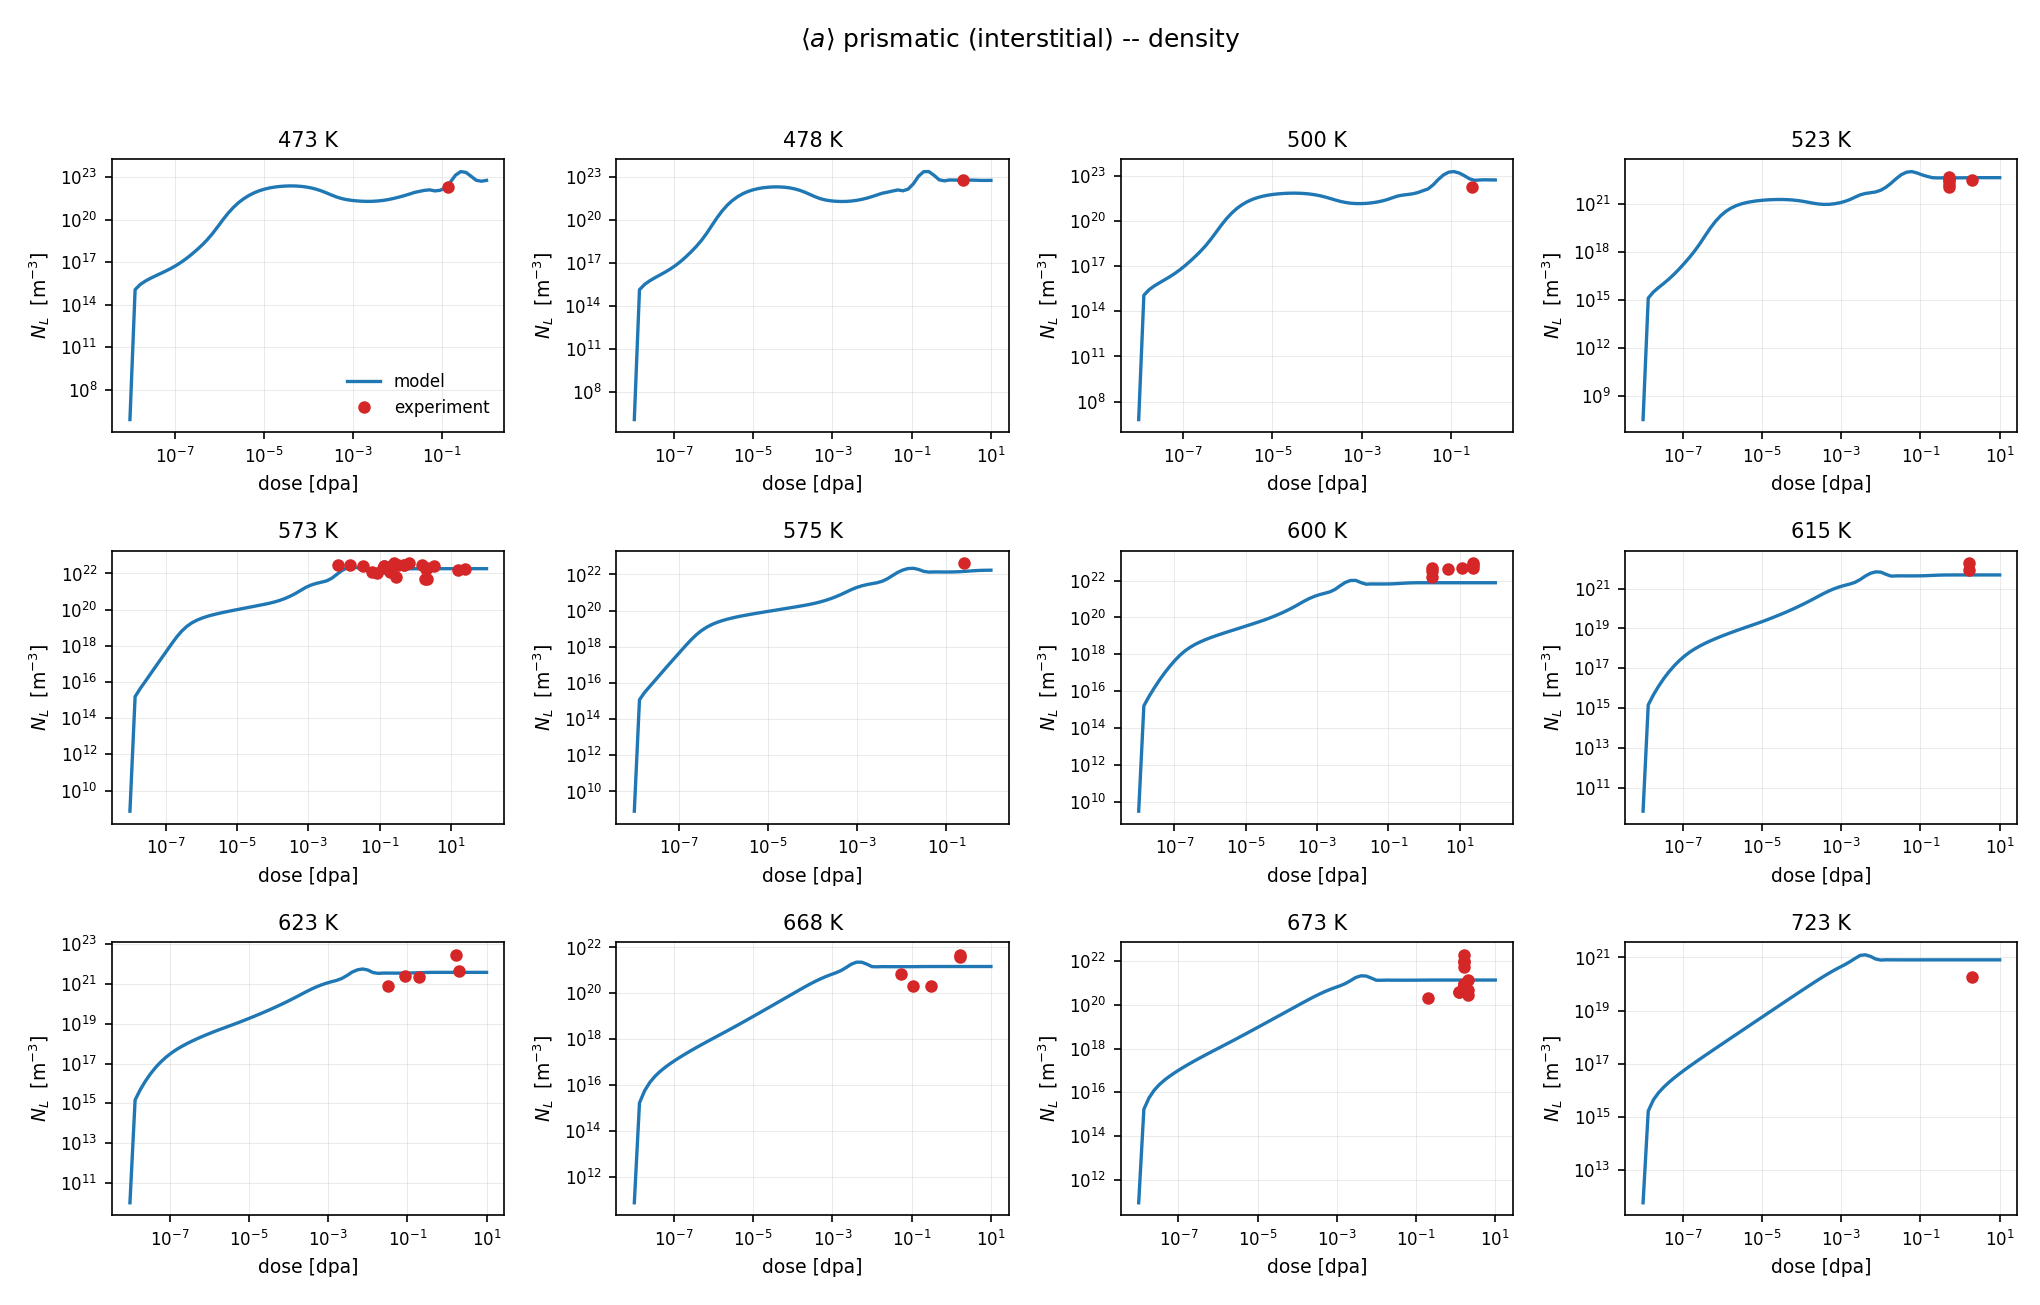
\includegraphics[width=\textwidth]{figures/fit_A_density.png}
\end{minipage}\hfill
\begin{minipage}{0.49\textwidth}\centering
  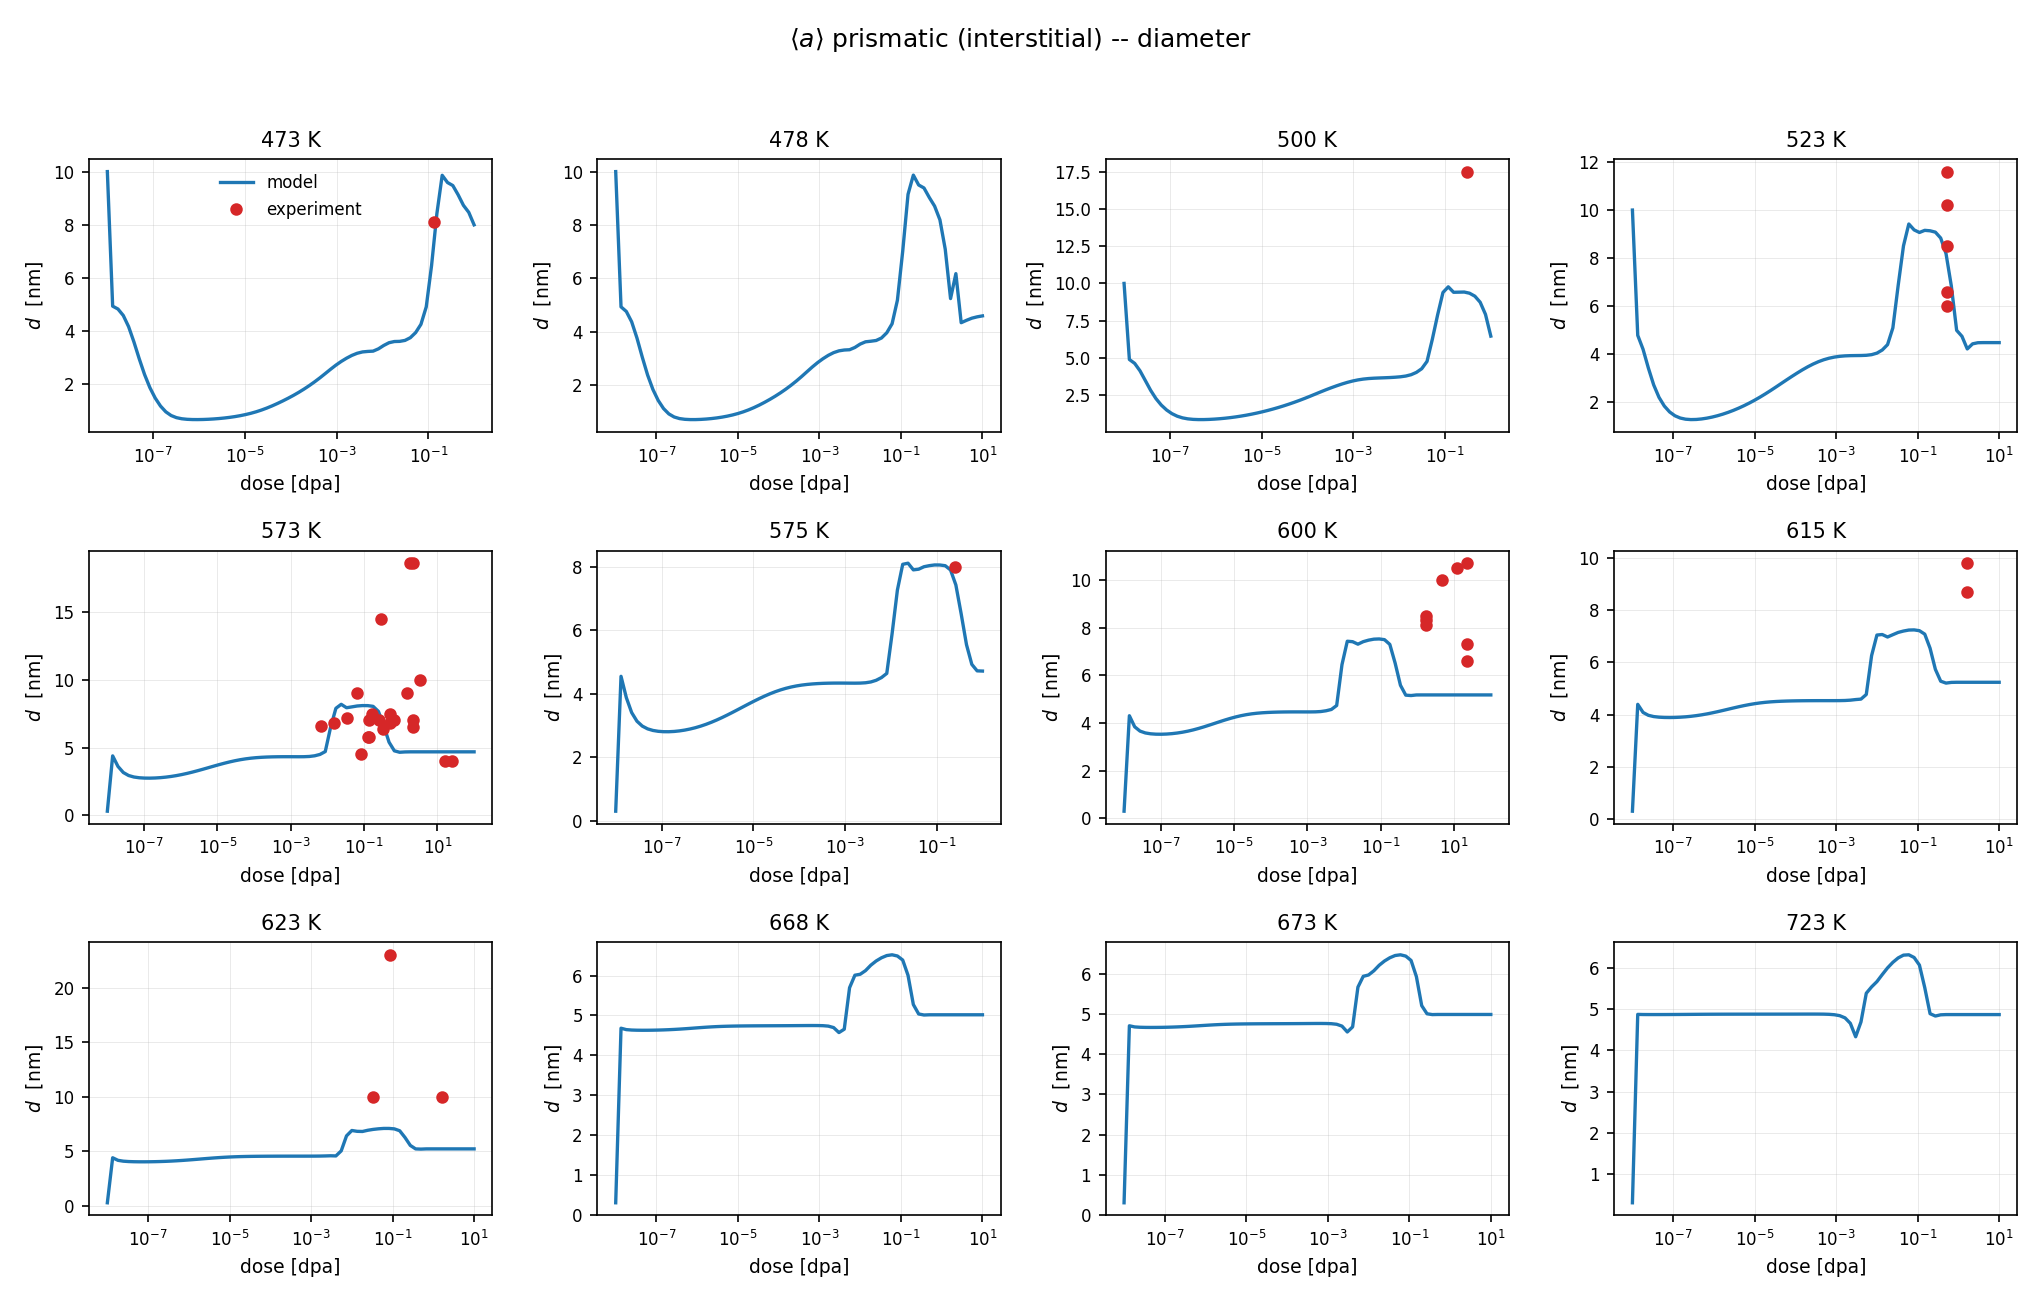
\includegraphics[width=\textwidth]{figures/fit_A_diameter.png}
\end{minipage}
\caption{Prismatic \aloop{} loops by temperature: number density (left) and
mean diameter (right), 71 and 44 points.}
\label{fig:fit-A}
\end{figure}

\begin{figure}[htbp]
\centering
\begin{minipage}{0.49\textwidth}\centering
  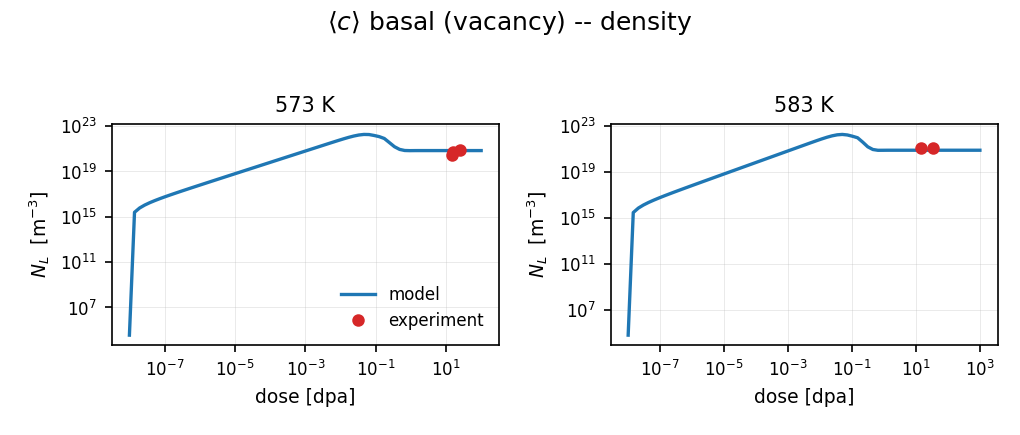
\includegraphics[width=\textwidth]{figures/fit_C_density.png}
\end{minipage}\hfill
\begin{minipage}{0.49\textwidth}\centering
  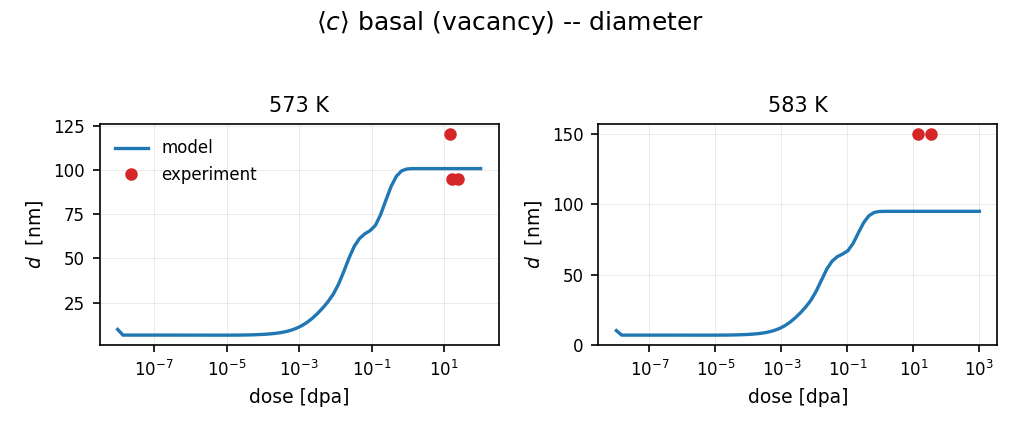
\includegraphics[width=\textwidth]{figures/fit_C_diameter.png}
\end{minipage}
\caption{Basal \cloop{} loops against the five available measurements, all above
14\,dpa; below that the model extrapolates.}
\label{fig:fit-C}
\end{figure}

\begin{figure}[htbp]
\centering
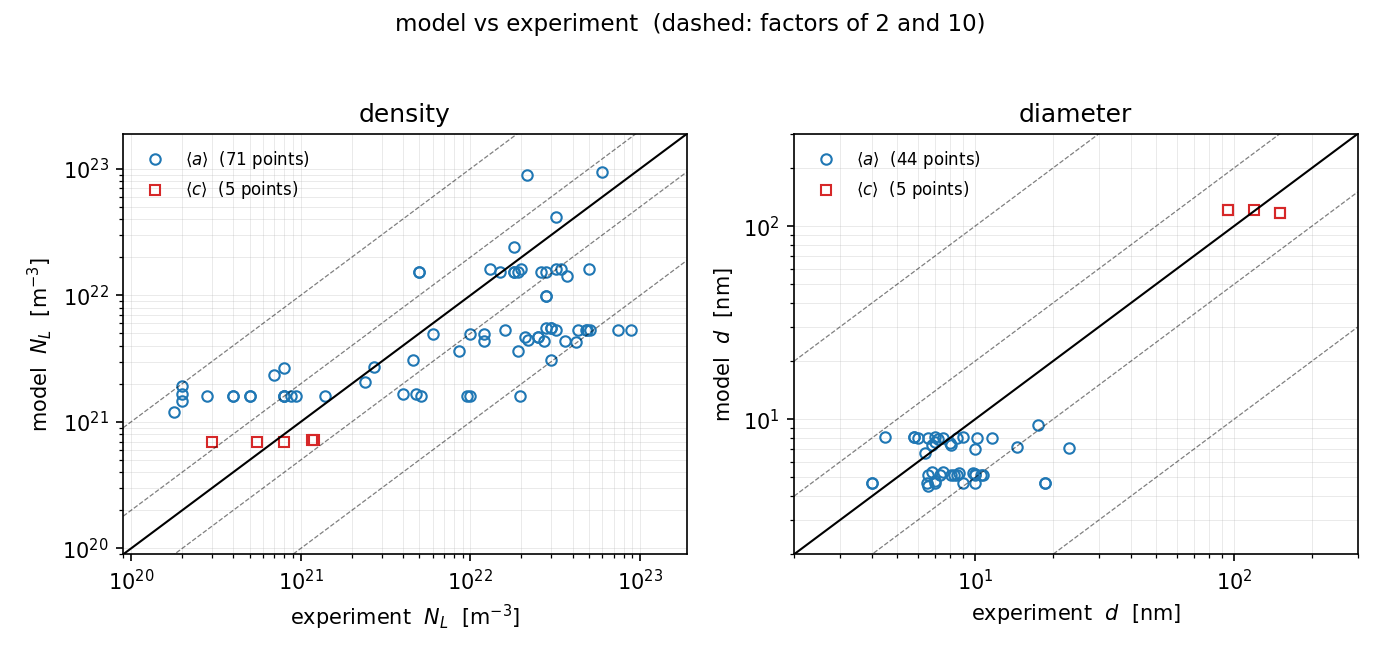
\includegraphics[width=0.62\textwidth]{figures/fit_parity.png}
\caption{Parity plot over all 78 measurements. The diagonal is exact agreement
and the dotted lines a factor of three.}
\label{fig:parity}
\end{figure}

\begin{table}[htbp]
\caption{The calibrated parameter set. The transport anisotropies are
\emph{inputs}, \cref{eq:pinned-pm}, not fitted values. $^{\dagger}$ rests on a
bound and is a constraint rather than an optimum (\cref{sec:bias-caveat});
$^{\ddagger}$ was not moved from the seed.}
\label{tab:fitted}
\centering\small
\begin{tabular}{@{}lr@{\qquad}lr@{\qquad}lr@{}}
\toprule
Parameter & Value & Parameter & Value & Parameter & Value \\
\midrule
\multicolumn{6}{@{}l}{\emph{transport, fixed by \cref{eq:pinned-pm}}}\\
$p^{v}$ & 1.0200 & $p^{i}$ & 0.7000 & $p^{2i}=p^{3i}$ & 0.7000 \\
\midrule
\multicolumn{6}{@{}l}{\emph{calibrated}}\\
$Z^{0}_{v}$ & 1.3000$^{\dagger}$ & $c_{LL}^{a}$ & 4.7720 & $\varepsilon_{2i}$ & 0.0010$^{\dagger}$ \\
$Z^{0}_{i}$ & 0.8935 & $c_{LL}^{c}$ & 1.2386 & $\varepsilon_{3i}$ & 0.007376 \\
$\xi_{c}$   & 2.0000$^{\dagger}$ & $c_{LN}^{a}$ & 94.615 & $\varepsilon_{iL}$ & 0.000200$^{\dagger}$ \\
$Z_N$       & 1.0100$^{\ddagger}$ & $c_{LN}^{c}$ & 1.1198 & $\varepsilon_{vL}$ & 0.005000$^{\dagger}$ \\
$E^{m}_{i}$ (eV) & 0.8970 & $\kappa_{LL}$ & 20.000$^{\dagger}$ & $m^{\mathrm{nuc}}_{a}$ & 53.79 \\
$E^{m}_{2i}$ (eV) & 1.3629$^{\ddagger}$ & $\kappa_{LN}$ & 4.0000$^{\dagger}$ & $m^{\mathrm{nuc}}_{c}$ & 400.00$^{\dagger}$ \\
$E^{b}_{2i}$ (eV) & 0.9570$^{\ddagger}$ & $m_{\min}$ & 5.8286 & $c_{\rho_N}$ & 0.0010$^{\ddagger}$ \\
$\chi$ & 1.0000$^{\ddagger}$ & $m_{\mathrm{vanish}}$ & 14.04 & $k_{\rho_N}^{\mathrm{rec}}$ & $3.5\times10^{-5}$$^{\ddagger}$ \\
 & & $\nu_{\mathrm{vanish}}$ & 0.0010$^{\dagger}$ & & \\
\bottomrule
\end{tabular}
\end{table}

\subsection{What the calibration does not achieve}
\label{sec:atrend}\label{sec:bias-caveat}

The \aloop{} mean conceals the one clear deficiency. Resolved by temperature the
model runs high at both ends and low in the middle:

\begin{center}
\begin{tabular}{@{}lrrrrrrr@{}}
\toprule
$T$ (K) & 473 & 523 & 573 & 575 & 600 & 623 & 673 \\
\midrule
$N_a/N_a^{\exp}$ & 1.29 & 1.66 & 0.88 & 0.35 & \textbf{0.17} & 1.01 & 1.17 \\
$d_a/d_a^{\exp}$ & 0.59 & 1.37 & 1.34 & 1.38 & 1.17 & 0.77 & --- \\
\bottomrule
\end{tabular}
\end{center}

Near $600\,$K the prismatic density is still a factor of six low, and
$573$--$600\,$K is the band \cref{sec:results} runs in. This is not a stage that
failed to converge: four independent searches, seeded differently and carrying
the levers a screen identifies as having the right temperature signature ---
$E^{m}_{i}$, the two coalescence exponents and the cascade partitions
$\varepsilon_{2i}$, $\varepsilon_{3i}$, each of which lowers the low-temperature
end while raising the middle --- all reach the same place, the mean improving
and the middle band not. The deficiency survives the change of anisotropy, the
diameter weighting and its own dedicated stage. Two readings remain, and these
data cannot separate them: the prismatic nucleation term may carry the wrong
temperature dependence, being a cascade partition with none of its own, or the
high-temperature points may not measure the same population, since above
$\sim\!650\,$K the reported \aloop{} loops include vacancy loops --- already the
reason their diameters are excluded from \cref{tab:targets}. The second is
testable by character-resolved measurements at $600$--$700\,$K, and is the more
useful thing to ask of an experiment.

Fixing $p^{m}$ removed four rails and not the pressure that produced them. Four
parameters in \cref{tab:fitted} rest on the edge of the box: $Z^{0}_{v}=1.30$
and the basal sink scale $\xi_{c}=2.00$ at their ceilings, and both coalescence
exponents $\kappa_{LL}=20$, $\kappa_{LN}=4$ at theirs. Their pattern is more
informative than any one of them. $Z^{0}_{v}$ and $\xi_{c}$ both multiply the
basal capture rate and are nearly degenerate, so they are one statement, not
two: given a stated anisotropy the model cannot deliver the measured basal
population without a prefactor no transport argument supplies. That locates the
shortfall in the capture prefactor and not the diffusion tensor. The two
$\kappa$ on their ceilings say the same of coalescence --- the fit wants more
overlap removal than the admissible range allows. That is sharper than the earlier
calibrations supported --- with $p^{v}$ free it absorbed the discrepancy and the
diagnosis stopped at ``the fit wants an implausible anisotropy''; pinned, it
reappears where it cannot be mistaken for transport. Atomistic constraints on
$p^{m}$ would confirm or refute \cref{eq:pinned-pm} directly, and
\cref{eq:Emsplit} would accept them without refitting anything else.

Two caveats on carrying this set into \cref{sec:results}. The fit is the
march's slow step term for term --- one templated function, the same binary and
switches, differing only in whether the mobile species are frozen --- so the
parameters transfer exactly. What does not transfer is what the $0$-D cannot
see: there the vacancy pool is free and re-equilibrates where the march pins it
to the fast solve, and the two need not move a quantity the same way. And the
shifts above target a $3$-D interior not yet re-measured with this set.

\section{Results: a 500\,nm Hexagonal Single Crystal to 10\,dpa}
\label{sec:results}

Every result below comes from one calculation: the calibrated parameter set of
\cref{tab:fitted}, all nine families, three moments each, peripheral emission
active, the basal chain inactive, and the grain-boundary loop channel of
\cref{sec:gb-loops} active. Conditions are $T=573\,$K,
$G=10^{-7}\,\mathrm{dpa\,s^{-1}}$, zero applied stress, and eight dose intervals
from $10^{-4}$ to 10\,dpa. Where a comparison is drawn against the same case
\emph{without} the loop channel, that companion differs in nothing else.

\subsection{Geometry, discretization and system size}
\label{sec:geometry}

The domain is a hexagonal prism of 500\,nm across flats and 800\,nm along
$[0001]$, meshed with a refined boundary layer 100\,nm deep in which the target
element size falls from 60 to 20\,nm (\cref{fig:mesh}). The refinement is not
cosmetic: \cref{sec:results-mobile} measures interstitial boundary layers of
$16$--$28\,$nm, so an unrefined mesh at $60\,$nm would resolve the steepest
gradient in the problem with a single element.

\begin{figure}[htbp]
\centering
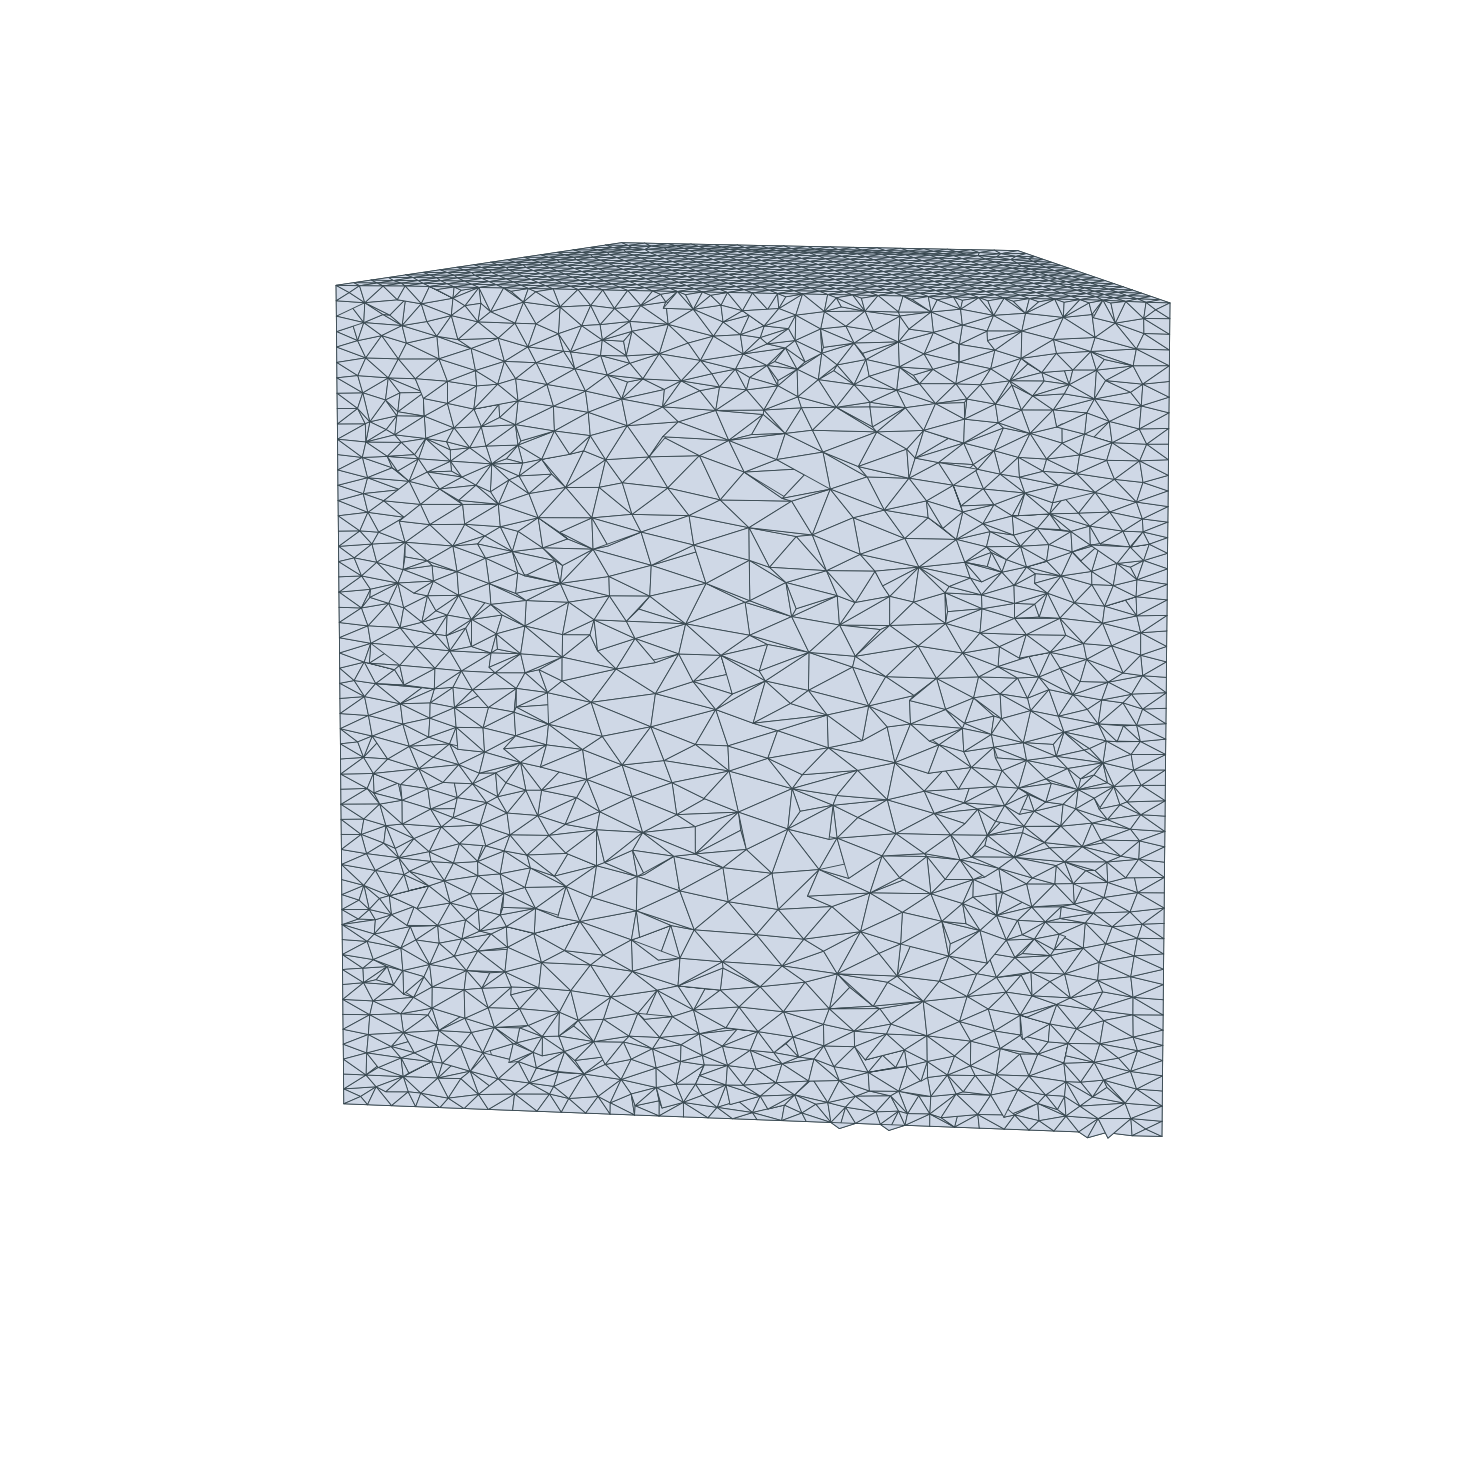
\includegraphics[width=0.55\textwidth]{figures/fe_mesh.png}
\caption{The finite-element mesh, cut in half so that the interior is visible:
60\,922 tetrahedra on 12\,581 mesh vertices. The refinement toward the six
prismatic faces and the two basal faces is the boundary layer, 100\,nm deep,
within which the element size falls from 60 to 20\,nm. Crystal axes as in
\cref{fig:hcp-cell}: $[10\bar10]$, $[\bar2\bar1\bar10]$ and $[0001]$.}
\label{fig:mesh}
\end{figure}

The cluster-dynamics trial functions live on second-order elements, so the field
nodes are more numerous than the mesh vertices: 90\,617 of them, filling a
crystal of $1.295\times10^{8}\,\mathrm{nm^{3}}$, or $5.568\times10^{9}$ atoms.
The resulting system sizes are those of \cref{tab:cost}: 362\,468 mobile
degrees of freedom solved as one coupled algebraic system eight times, and
2\,446\,659 immobile ones marched as 72\,928 independent 36-dimensional stiff
systems at each of 24 substeps --- $7.8\times10^{7}$ scalar ordinary differential
equations over the march, in 1\,h\,04\,m on 24 cores.

\textbf{The whole surface is a boundary.} No face is periodic, so every face
carries \cref{eq:bc}, and the maximum distance from any node to the nearest face
is 215\,nm --- the inradius, and the cap $R_{\max}$ used in \cref{eq:trunc}.

\subsection{Mobile defect fields}
\label{sec:results-mobile}

\Cref{fig:mobile} shows the four mobile species early in the transient
($10^{-4}\,$dpa) and at the end of the march (10\,dpa), on two orthogonal
mid-cuts. Every panel has the same structure --- an interior plateau and a
depleted shell --- and the differences between them are entirely in the width of
that shell and in the level of the plateau.

\begin{figure}[htbp]
\centering
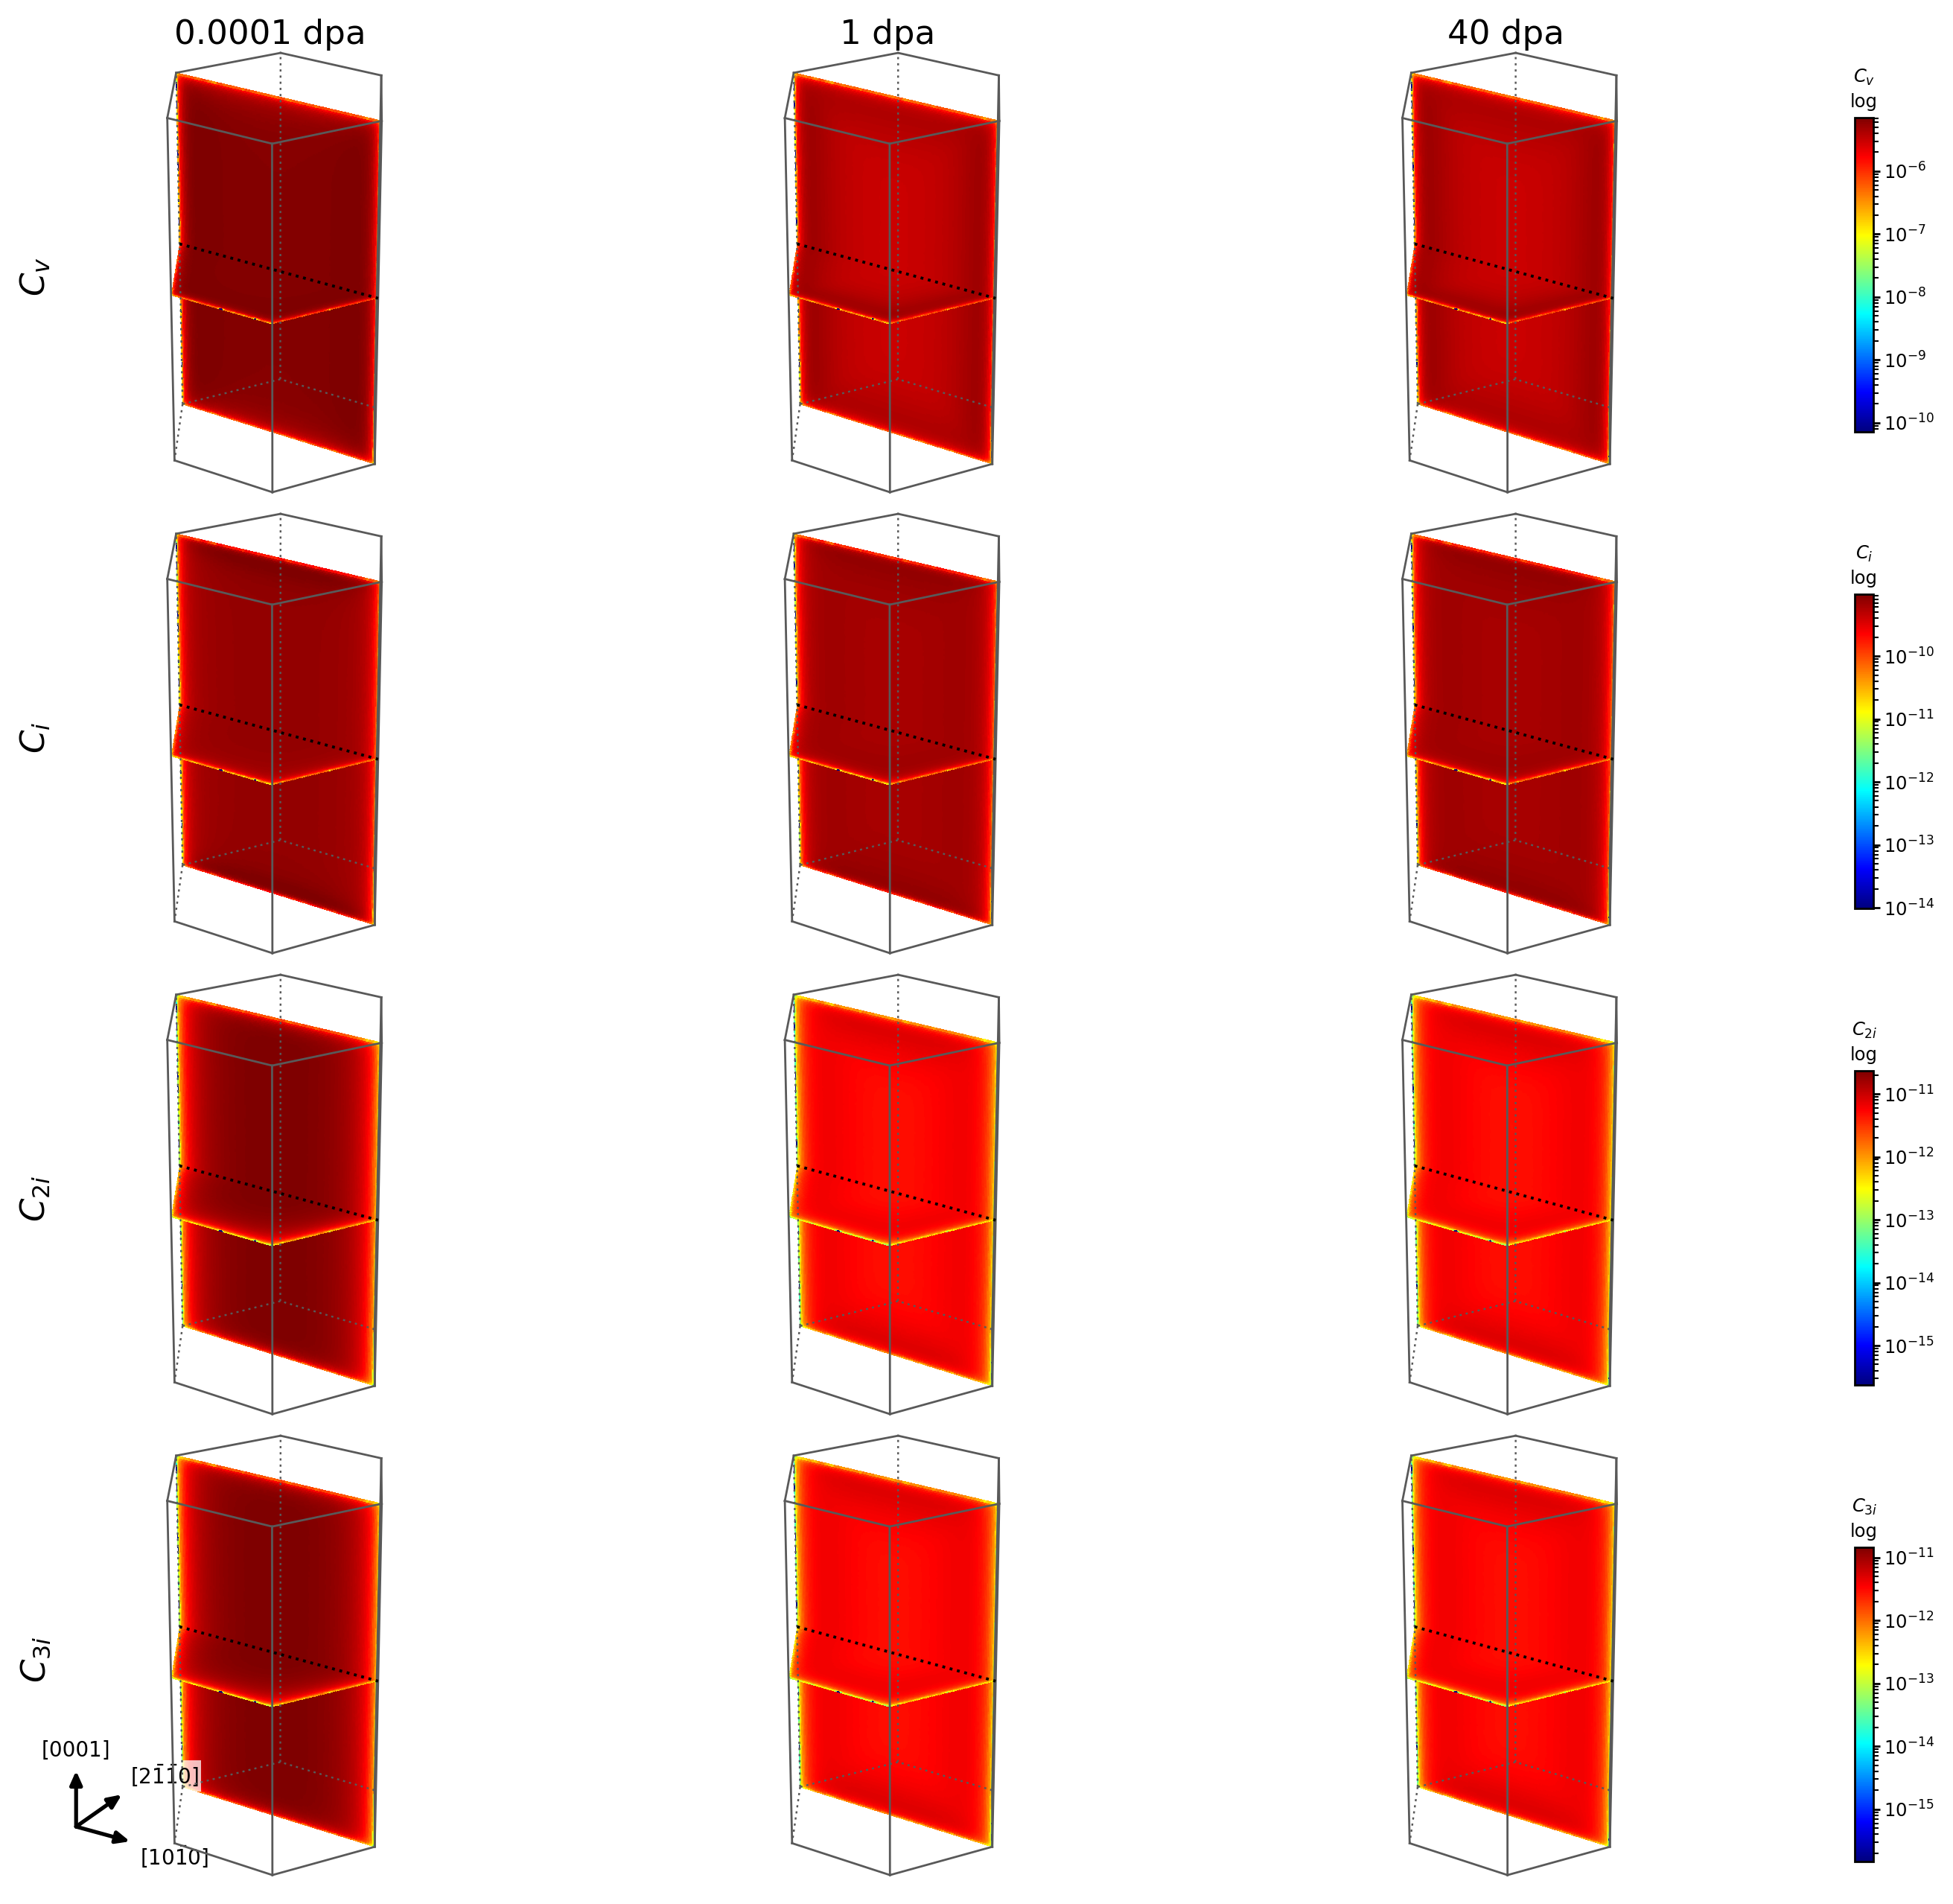
\includegraphics[width=\textwidth]{figures/mobile_early_late.png}
\caption{Mobile species at $10^{-4}\,$dpa (left) and 10\,dpa (right), on one
vertical and one horizontal mid-cut. Rows, top to bottom: $C_v$, $C_i$,
$C_{2i}$, $C_{3i}$; each row has its own logarithmic color scale, so levels are
comparable across dose within a row and not between rows. The interior plateau
falls and the depleted shell narrows between the two doses, both because the
sink density has risen.}
\label{fig:mobile}
\end{figure}

\paragraph{The boundary layer is a diffusion length and it orders the species.}
Measuring the layer as the distance at which the binned median recovers
$1-e^{-1}$ of the interior plateau:

\begin{center}
\begin{tabular}{@{}lrrrr@{}}
\toprule
Dose (dpa) & $C_v$ & $C_i$ & $C_{2i}$ & $C_{3i}$ \\
\midrule
$10^{-4}$ & 16.5\,nm & 27.5\,nm & 46.0\,nm & 46.0\,nm \\
$10^{-2}$ & 14.9\,nm & 27.5\,nm & 46.0\,nm & 46.0\,nm \\
$10$      &  8.0\,nm & 16.5\,nm & 18.2\,nm & 18.2\,nm \\
\bottomrule
\end{tabular}
\end{center}

Two readings, and both are consequences of $L\sim\sqrt{D/k^{2}}$ rather than of
anything fitted. \emph{Across species at fixed dose}, the layer widens with
mobility: the vacancy, least mobile, is depleted over the shortest distance,
while the interstitial clusters --- which reach a sink from further away ---
carry the widest layer. \emph{Across dose at fixed species}, every layer
narrows, by a factor of two between $10^{-4}$ and 10\,dpa, because $k^{2}$ has
grown with the loop population that the same calculation is building. The
boundary layer is therefore not a fixed geometric feature of the domain; it is a
running measure of the sink density, and it tightens as the microstructure
develops.

\paragraph{Anisotropy acts on the shape of the layer, not only its width.}
Because the domain has two basal faces and six prismatic ones, the layer can be
measured separately toward each set, using only the nodes for which that set is
the nearer boundary:

\begin{center}
\begin{tabular}{@{}lrrrr@{}}
\toprule
& \multicolumn{2}{c}{$10^{-4}$\,dpa} & \multicolumn{2}{c}{10\,dpa} \\
\cmidrule(lr){2-3}\cmidrule(lr){4-5}
Species & toward basal & toward prismatic & toward basal & toward prismatic \\
\midrule
$C_v$    & 84.8\,nm & 11.7\,nm & 24.0\,nm & 6.8\,nm \\
$C_i$    & 12.8\,nm & 28.8\,nm &  7.5\,nm & 18.3\,nm \\
$C_{2i}$ & 22.0\,nm & 45.2\,nm &  6.8\,nm & 24.0\,nm \\
$C_{3i}$ & 24.0\,nm & 45.2\,nm &  6.8\,nm & 24.0\,nm \\
\bottomrule
\end{tabular}
\end{center}

The vacancy layer is $7.2$ times \emph{wider} toward the basal faces than toward
the prismatic ones, which is the sign the fitted $p^{v}=1.6$ requires: vacancies
are $16.8$ times more mobile along $[0001]$ (\cref{eq:Dratio}), and a species
that reaches a sink from further away is depleted over a longer distance. The
scale expected from $L\sim\sqrt{D/k^{2}}$ is
$\sqrt{16.8}=4.1$, so the measured $7.2$ is not a clean reading of the
diffusivity ratio, and the interstitial rows show why. At $p^{i}=1.0$ the
interstitials diffuse isotropically, yet their layer is \emph{narrower} toward
the basal faces by a factor of $0.44$ --- an effect of domain shape rather than
of transport, since a node near a prismatic face is close to several faces at
once and is depleted more than its distance to the nearest one would suggest.
Anisotropy and geometry therefore act in opposite directions here, and only
their combination is directly observable.

Two consequences. First, an SRCD calculation on a shaped grain measures the
convolution of the diffusion tensor with the grain geometry, so extracting one
requires the other to be known --- which is an argument for calibrating $p^{m}$
atomistically rather than from a boundary-layer profile
(\cref{sec:conclusions}). Second, the narrowest layer in the problem is the
interstitial one toward a basal face, $7.5\,$nm at 10\,dpa, against a
$20\,$nm boundary element: the steepest gradient the calculation contains is
resolved by well under one element, and it is at exactly such a location that an
earlier calculation on this geometry drove a single node beyond the integrator's
reach (\cref{sec:failure}).

Interior median concentrations fall over the march --- $C_v$ from
$6.02\times10^{-6}$ to $2.29\times10^{-6}$, $C_i$ from $7.92\times10^{-10}$ to
$4.16\times10^{-10}$, and the clusters by nearly an order of magnitude --- which
is the signature of a rising sink density at constant production.

\subsection{Immobile fields and their moments}
\label{sec:results-moments}

\Cref{fig:moments-cf,fig:moments-a1} show the three carried moments of the
faulted basal family and of one prismatic interstitial variant, at the same two
doses. The three rows are not three views of one thing; they answer different
questions, and their spatial structures differ.

\begin{figure}[htbp]
\centering
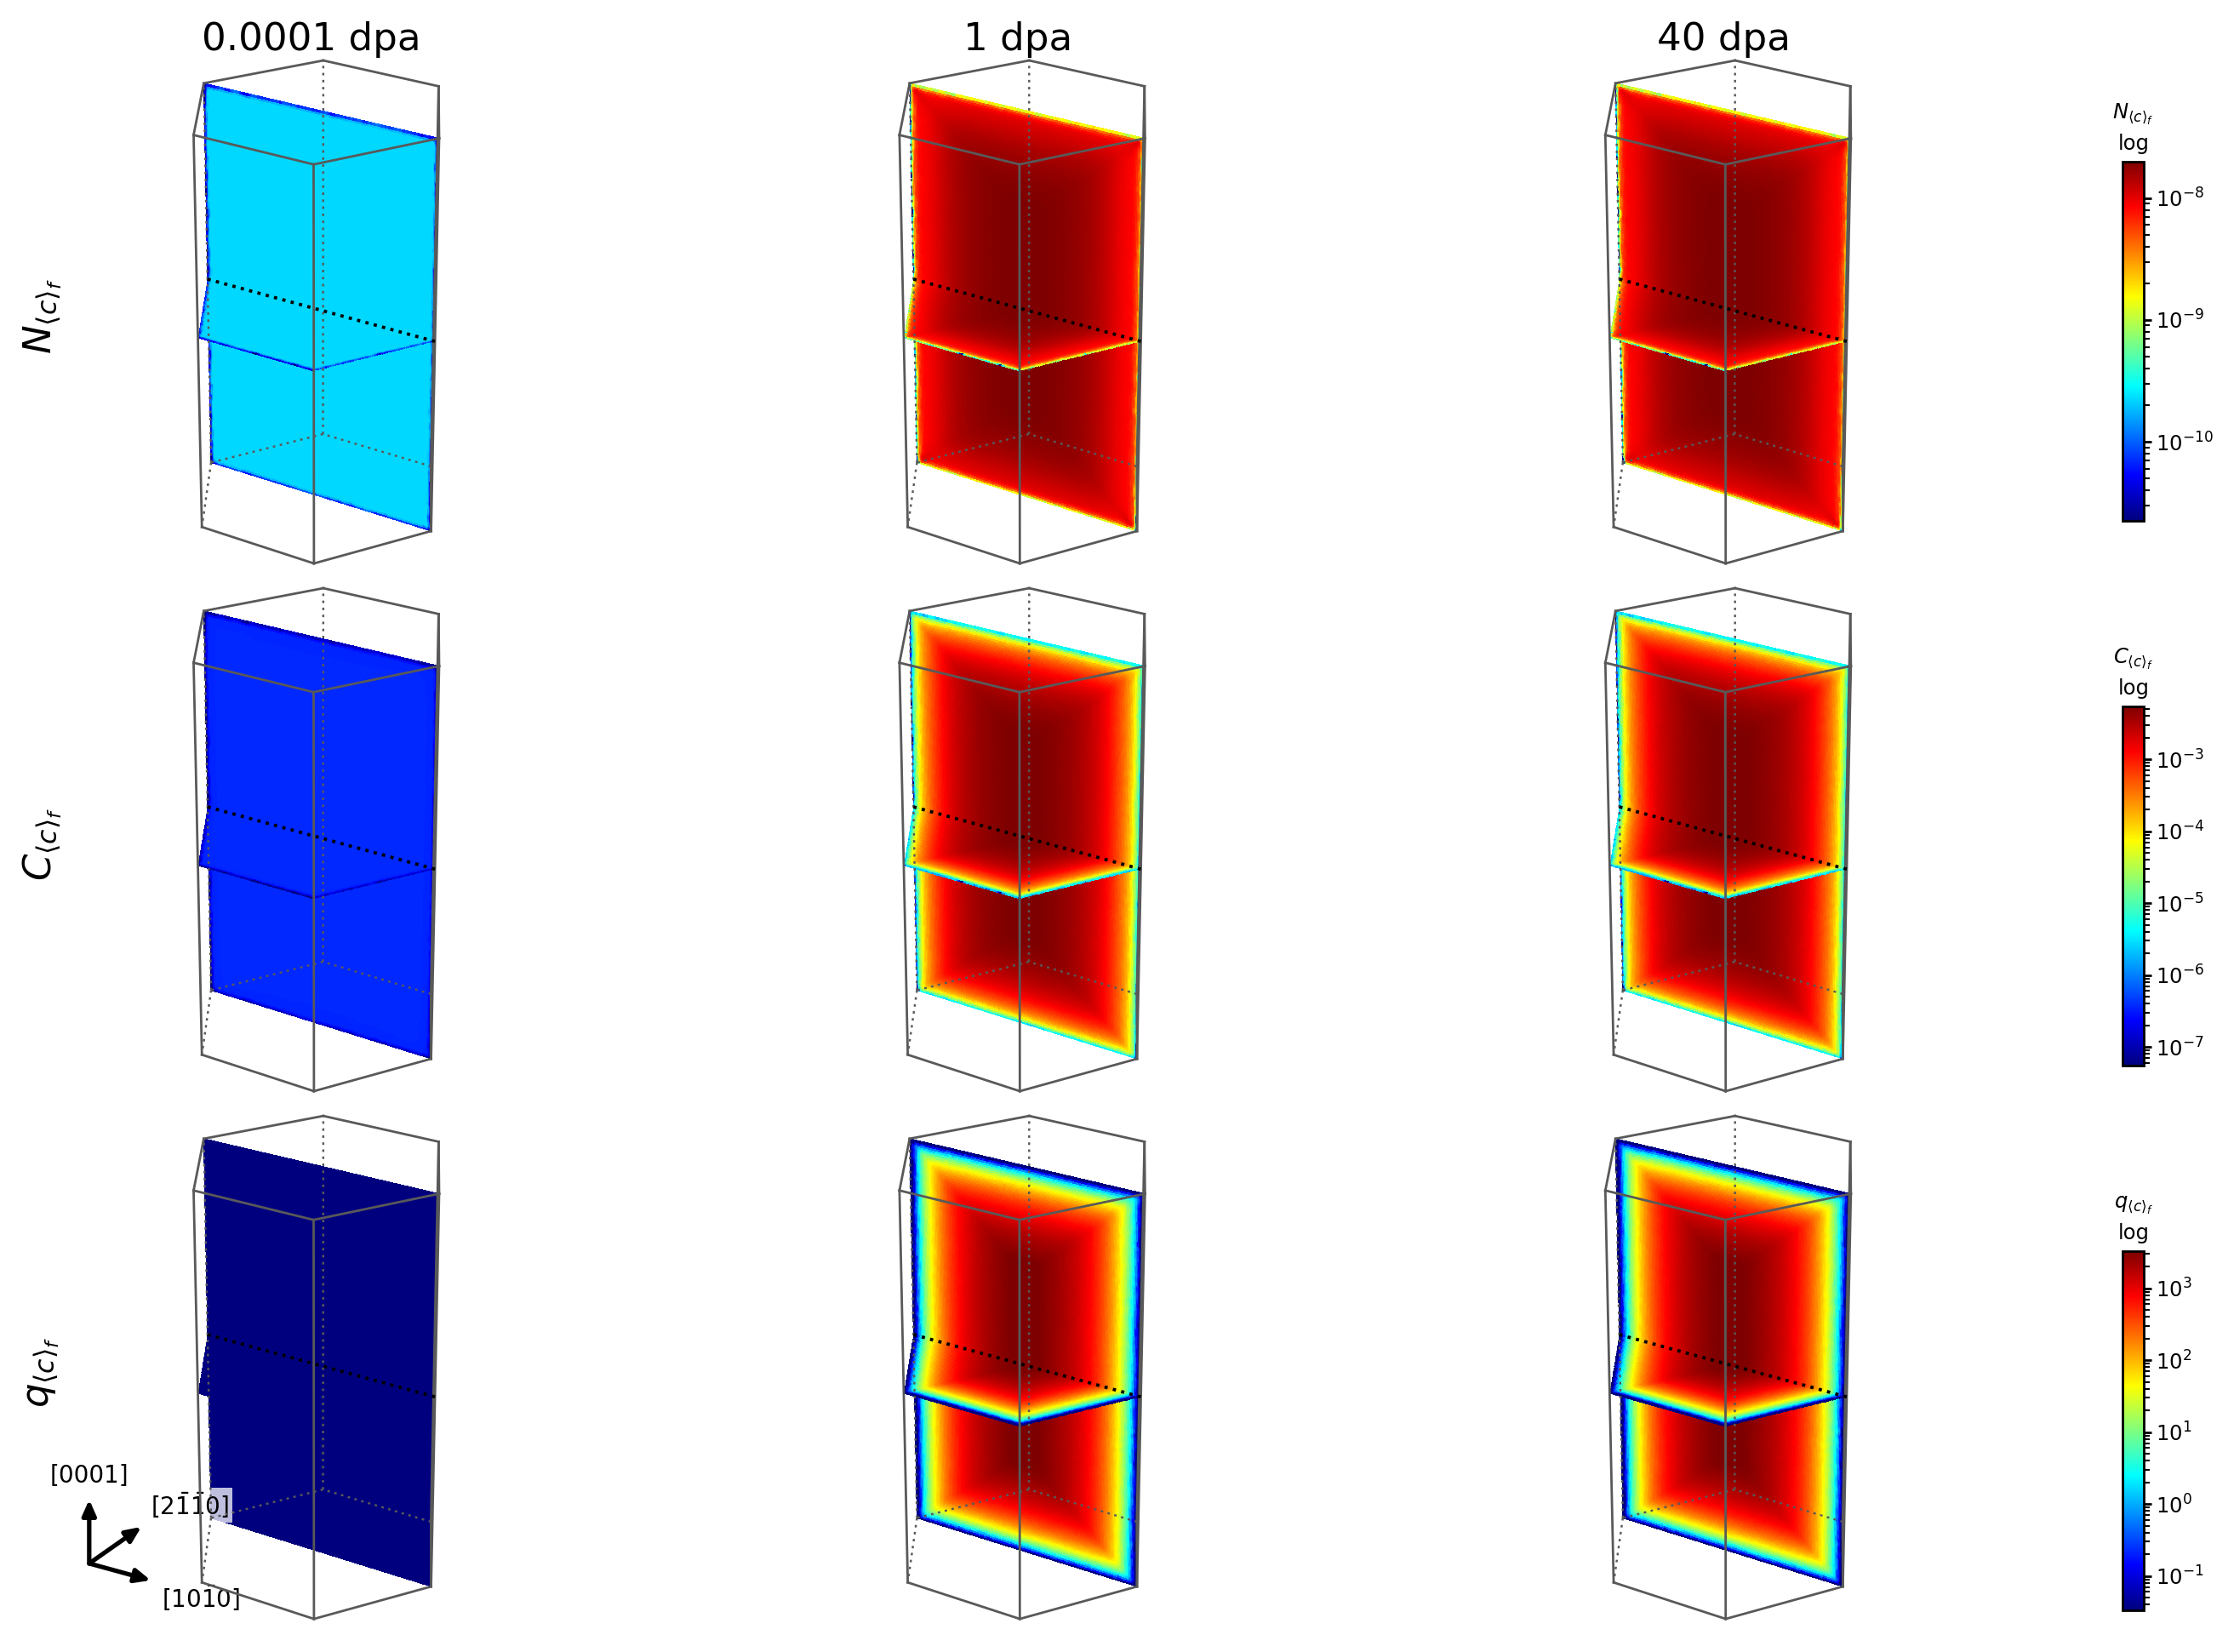
\includegraphics[width=\textwidth]{figures/moments_cf.png}
\caption{The basal faulted family $c_f$ at $10^{-4}$ and 10\,dpa: number density
$n$ (top), stored content $c$ (middle), second content $q$ (bottom).}
\label{fig:moments-cf}
\end{figure}

\begin{figure}[htbp]
\centering
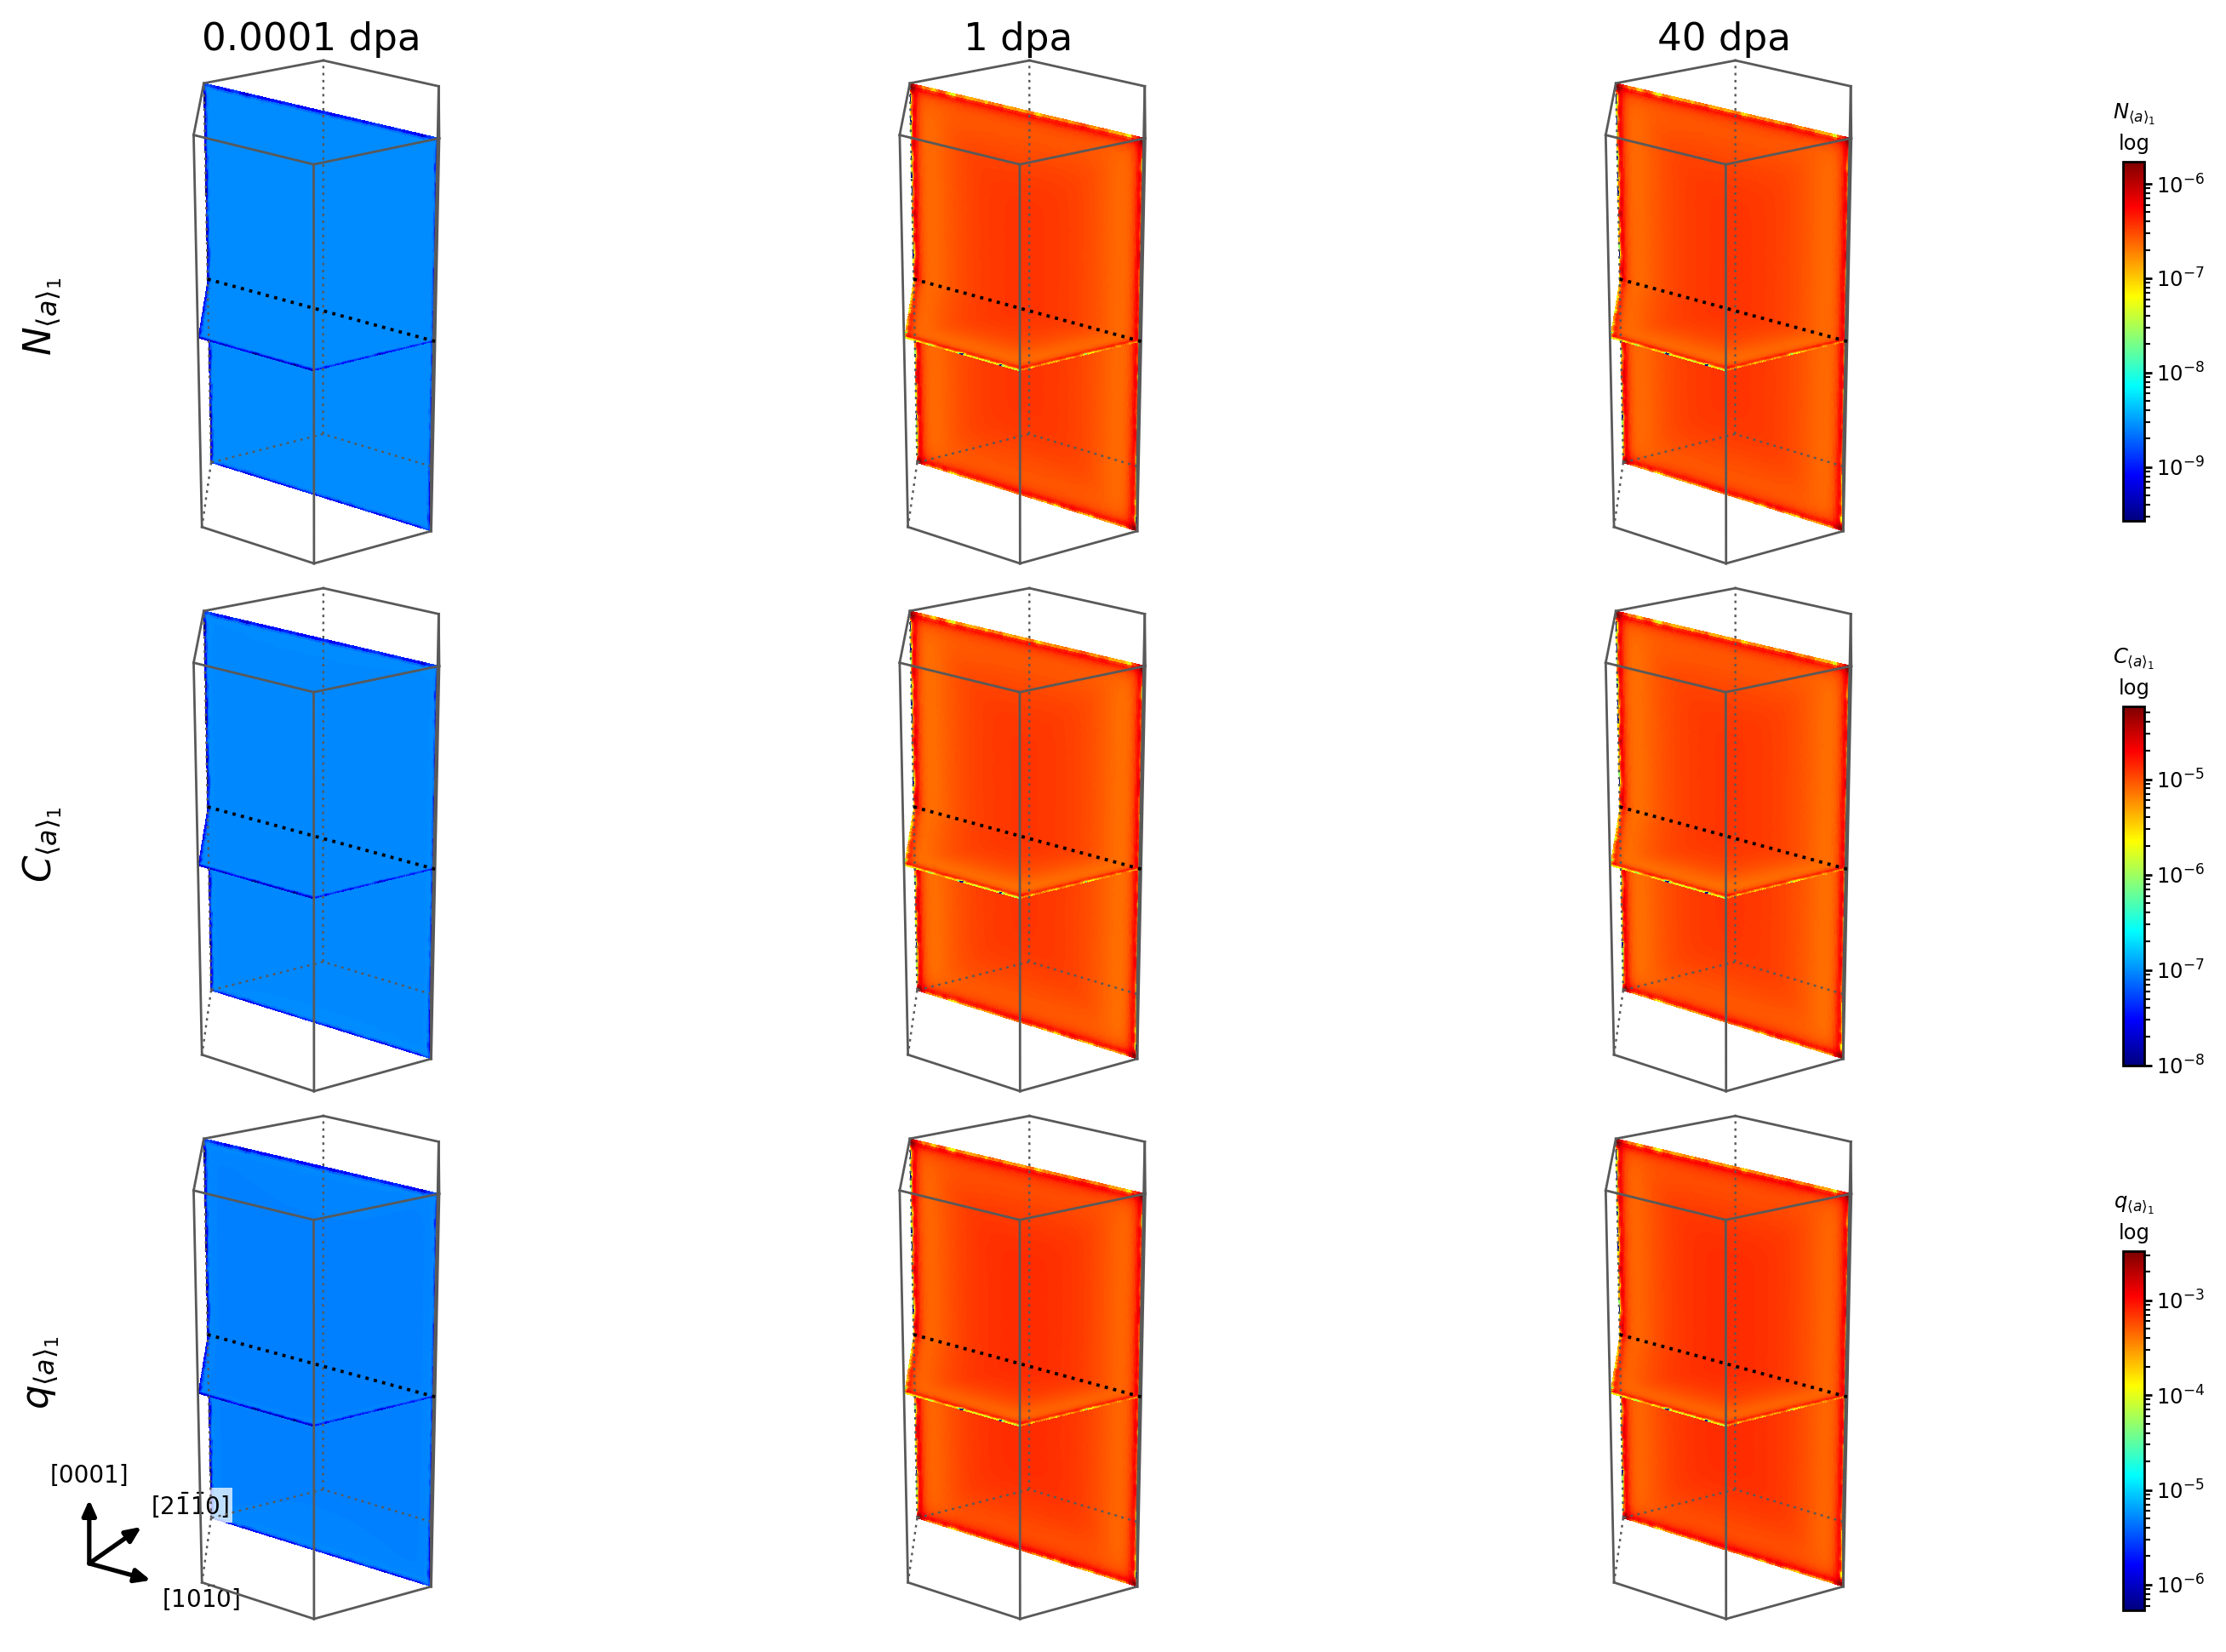
\includegraphics[width=\textwidth]{figures/moments_a1.png}
\caption{The prismatic interstitial variant $a_1$ at the same two doses, same
three moments. The variants $a_2$ and $a_3$ are identical at zero applied
stress and are not shown.}
\label{fig:moments-a1}
\end{figure}

\paragraph{Number is boundary-peaked, content is interior-peaked, and that is
the physics.} Cascade nucleation is spatially uniform, but the only channel that
removes a loop in the interior is coalescence, whose rate is driven by the
absorbed mobile flux --- and that flux vanishes where the Dirichlet condition
pins the mobile species. Near a boundary, loops are therefore nucleated and not
removed, so $n$ rises steeply toward the surface. They are also not \emph{fed},
because the same vanishing flux is what would grow them, so $c$ does not rise
with $n$ and the mean size $c/n$ collapses. Without the channel of
\cref{sec:gb-loops} that shell dominates every domain average, which is the
artifact \cref{sec:results-volume} quantifies.

\paragraph{The second moment does work, and it is realizable everywhere.} The
dispersion $\Delta_k=q n/c^{2}$ of \cref{eq:lognormal} must be $\ge1$ for the
three carried numbers to be the moments of any distribution at all. Measured
over the interior:

\begin{center}
\begin{tabular}{@{}lrrrrrr@{}}
\toprule
& \multicolumn{2}{c}{$c_f$} & \multicolumn{2}{c}{$a_1$}
& \multicolumn{2}{c}{$a_1^{v}$} \\
\cmidrule(lr){2-3}\cmidrule(lr){4-5}\cmidrule(lr){6-7}
Dose (dpa) & median & min & median & min & median & min \\
\midrule
$10^{-4}$ & 1.003 & 1.001 & 1.002 & 1.001 & 1.001 & 1.001 \\
$10^{-2}$ & 1.473 & 1.098 & 1.883 & 1.090 & 1.509 & 1.076 \\
$1$       & 1.559 & 1.250 & 2.724 & 2.442 & 2.215 & 2.112 \\
$10$      & 1.585 & 1.266 & 2.705 & 2.439 & 2.175 & 2.104 \\
\bottomrule
\end{tabular}
\end{center}

Three things follow. At $10^{-4}\,$dpa every family is monodisperse to
three decimal places, as it must be --- the loops present are all fresh nuclei
deposited at $m^{\mathrm{nuc}}_k$. By 1\,dpa the prismatic distribution has
broadened to $\Delta=2.72$, i.e. $s=\sqrt{\ln\Delta}=1.00$, a log-normal a full
decade wide at $\pm1\sigma$: a model carrying only $n$ and $c$ would represent
that population by a single size. And $\Delta\ge1$ holds at \emph{every}
interior node at every dose, minimum 1.001, which is the check that the channels
debiting $q$ are consistent with those debiting $n$ and $c$ --- a check that no
tolerance can substitute for, since $\Delta<1$ is not an inaccuracy but a
statement that the state is not a moment triple.

The basal family broadens less than the prismatic one ($1.59$ against $2.71$)
because its number loss is dominated by the boundary channel, which removes the
large end and therefore \emph{narrows} what remains, while the prismatic family
broadens under growth with no comparable truncation.

\subsection{Global conservation}
\label{sec:results-conservation}

The six atom-balance accumulators integrate the production, recombination and
sink absorption of each character, and the two accumulators of
\cref{sec:gb-loops} integrate the loop content taken by the boundary. In a
spatially resolved calculation on a Dirichlet domain the balance cannot close on
those channels alone, and the residual is not solver error: it is the atoms that
left through the surface as \emph{mobile} species. The magnitude settles the
matter --- nothing in an integration at $\mathrm{rtol}=10^{-6}$ is tens of
percent wrong.

\Cref{tab:conservation} is the balance over the whole march, per host atom.

\begin{table}[htbp]
\caption{The atom balance over $0\to10\,$dpa, volume-averaged, per host atom.
Production and recombination are exactly equal between the characters, as
Frenkel-pair production and recombination must be. The two channels that differ
are where the physics is: the network absorbs more interstitials than vacancies
(the bias), and the boundary absorbs vacancy \emph{loops} 60 times more than
interstitial ones.}
\label{tab:conservation}
\centering
\begin{tabular}{@{}lrrrr@{}}
\toprule
Channel & interstitial & vacancy & \%\,prod ($i$) & \%\,prod ($v$) \\
\midrule
produced                  & 10.0000 & 10.0000 & 100.00 & 100.00 \\
recombined                &  5.0832 &  5.0832 &  50.83 &  50.83 \\
absorbed at the network   &  0.7885 &  0.5908 &   7.88 &   5.91 \\
\textbf{loops at the boundary} & \textbf{0.0085} & \textbf{0.5123}
                          & \textbf{0.08} & \textbf{5.12} \\
stored in the microstructure & 0.0000 & 0.0020 & 0.00 & 0.02 \\
\midrule
mobile flux to the boundary (by difference)
                          &  4.1198 &  3.8117 &  41.20 &  38.12 \\
\bottomrule
\end{tabular}
\end{table}

Three readings.

\textbf{Both columns close on production.} $10.0000 = 5.0832+0.7885+0.0085+
0.0000+4.1198$ and likewise for the vacancies, so once the loop channel is
carried explicitly, what remains in the residual is the mobile flux alone and
the two do not contaminate each other. Before that channel was booked
separately, its 5.1\% of vacancy production was silently absorbed into the
residual, and because the residual is closure by difference, nothing looked
wrong.

\textbf{The boundary is the dominant sink, by a wide margin.} It takes
$41\%$ and $38\%$ of production as mobile species, against $7.9\%$ and $5.9\%$
at the network. That is a property of the geometry --- a 500\,nm grain with every
face absorbing --- and it is precisely what a mean-field model represents by a
single $k^{2}_{gb}$ and cannot resolve.

\textbf{The loop channel is strongly asymmetric.} It removes $0.512$ vacancies
per atom against $0.0085$ interstitials, a factor of 60. The asymmetry is
geometric, not biased: \cloop{} loops reach a mean radius of $25\,$nm where
\aloop{} loops reach $3\,$nm, so a basal loop intersects a face from far deeper
inside the crystal. Note also that the boundary removes \emph{250 times more}
vacancy loop content than the microstructure retains ($0.512$ against $0.0020$),
which is the quantitative form of the statement that on this grain size the
loop population is boundary-controlled.

\Cref{fig:conservation} shows the channels against dose and the fractional
decomposition. The fractions sum to unity once the boundary channels are
included; without them the sum reached only $\sim0.3$.

\begin{figure}[htbp]
\centering
\begin{minipage}{0.49\textwidth}\centering
  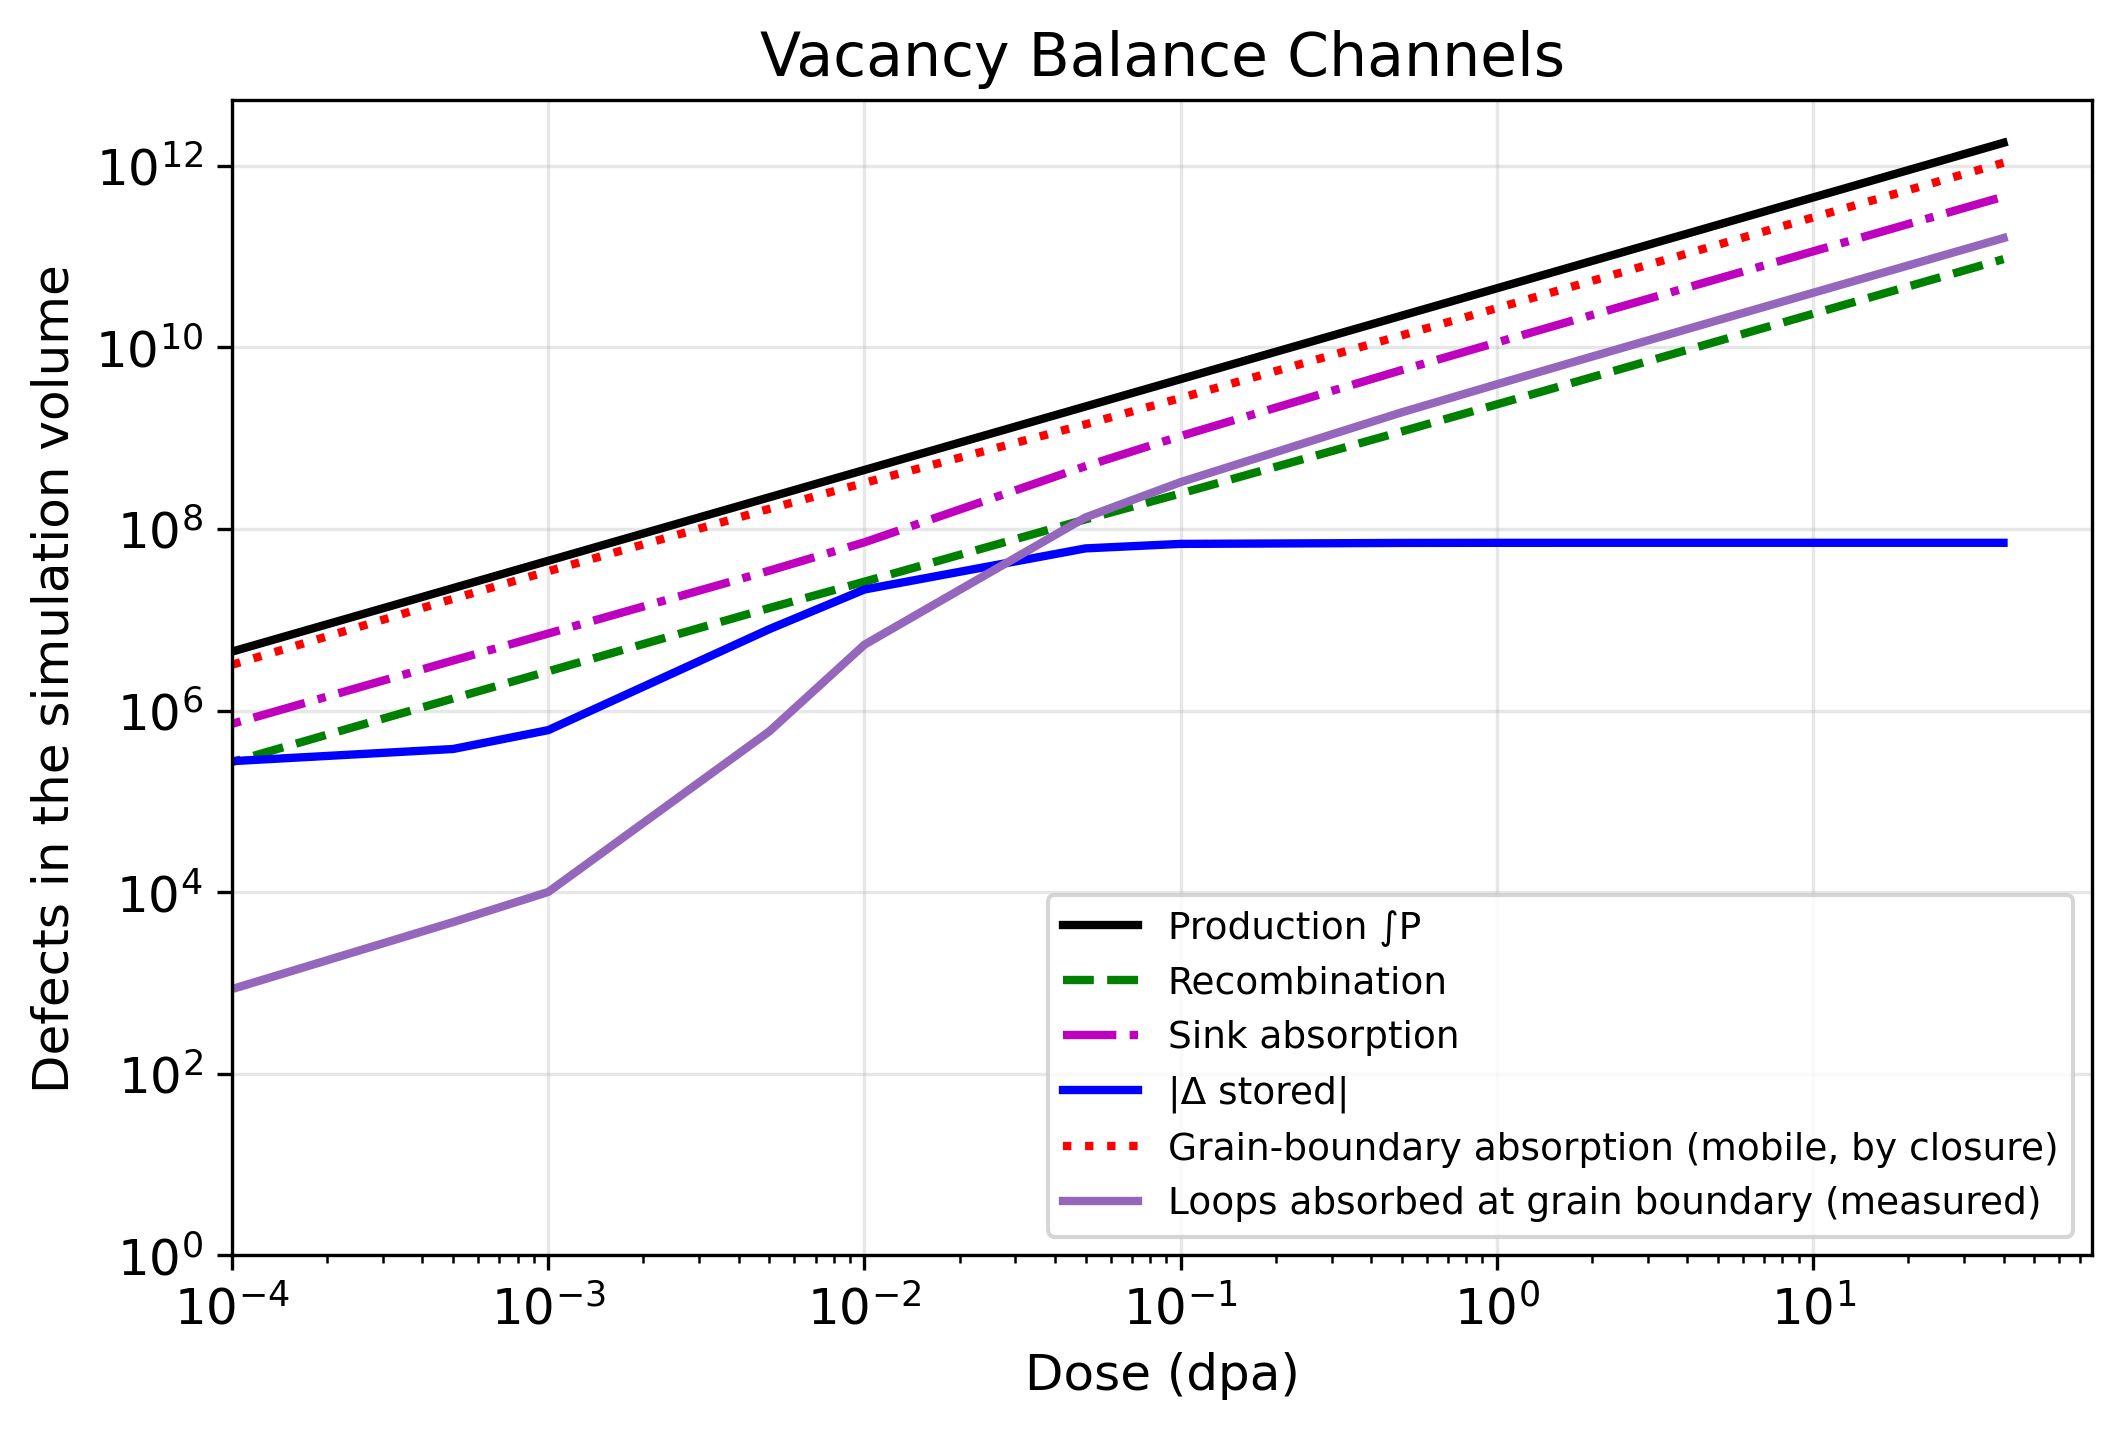
\includegraphics[width=\textwidth]{figures/conservation_v.png}
\end{minipage}\hfill
\begin{minipage}{0.49\textwidth}\centering
  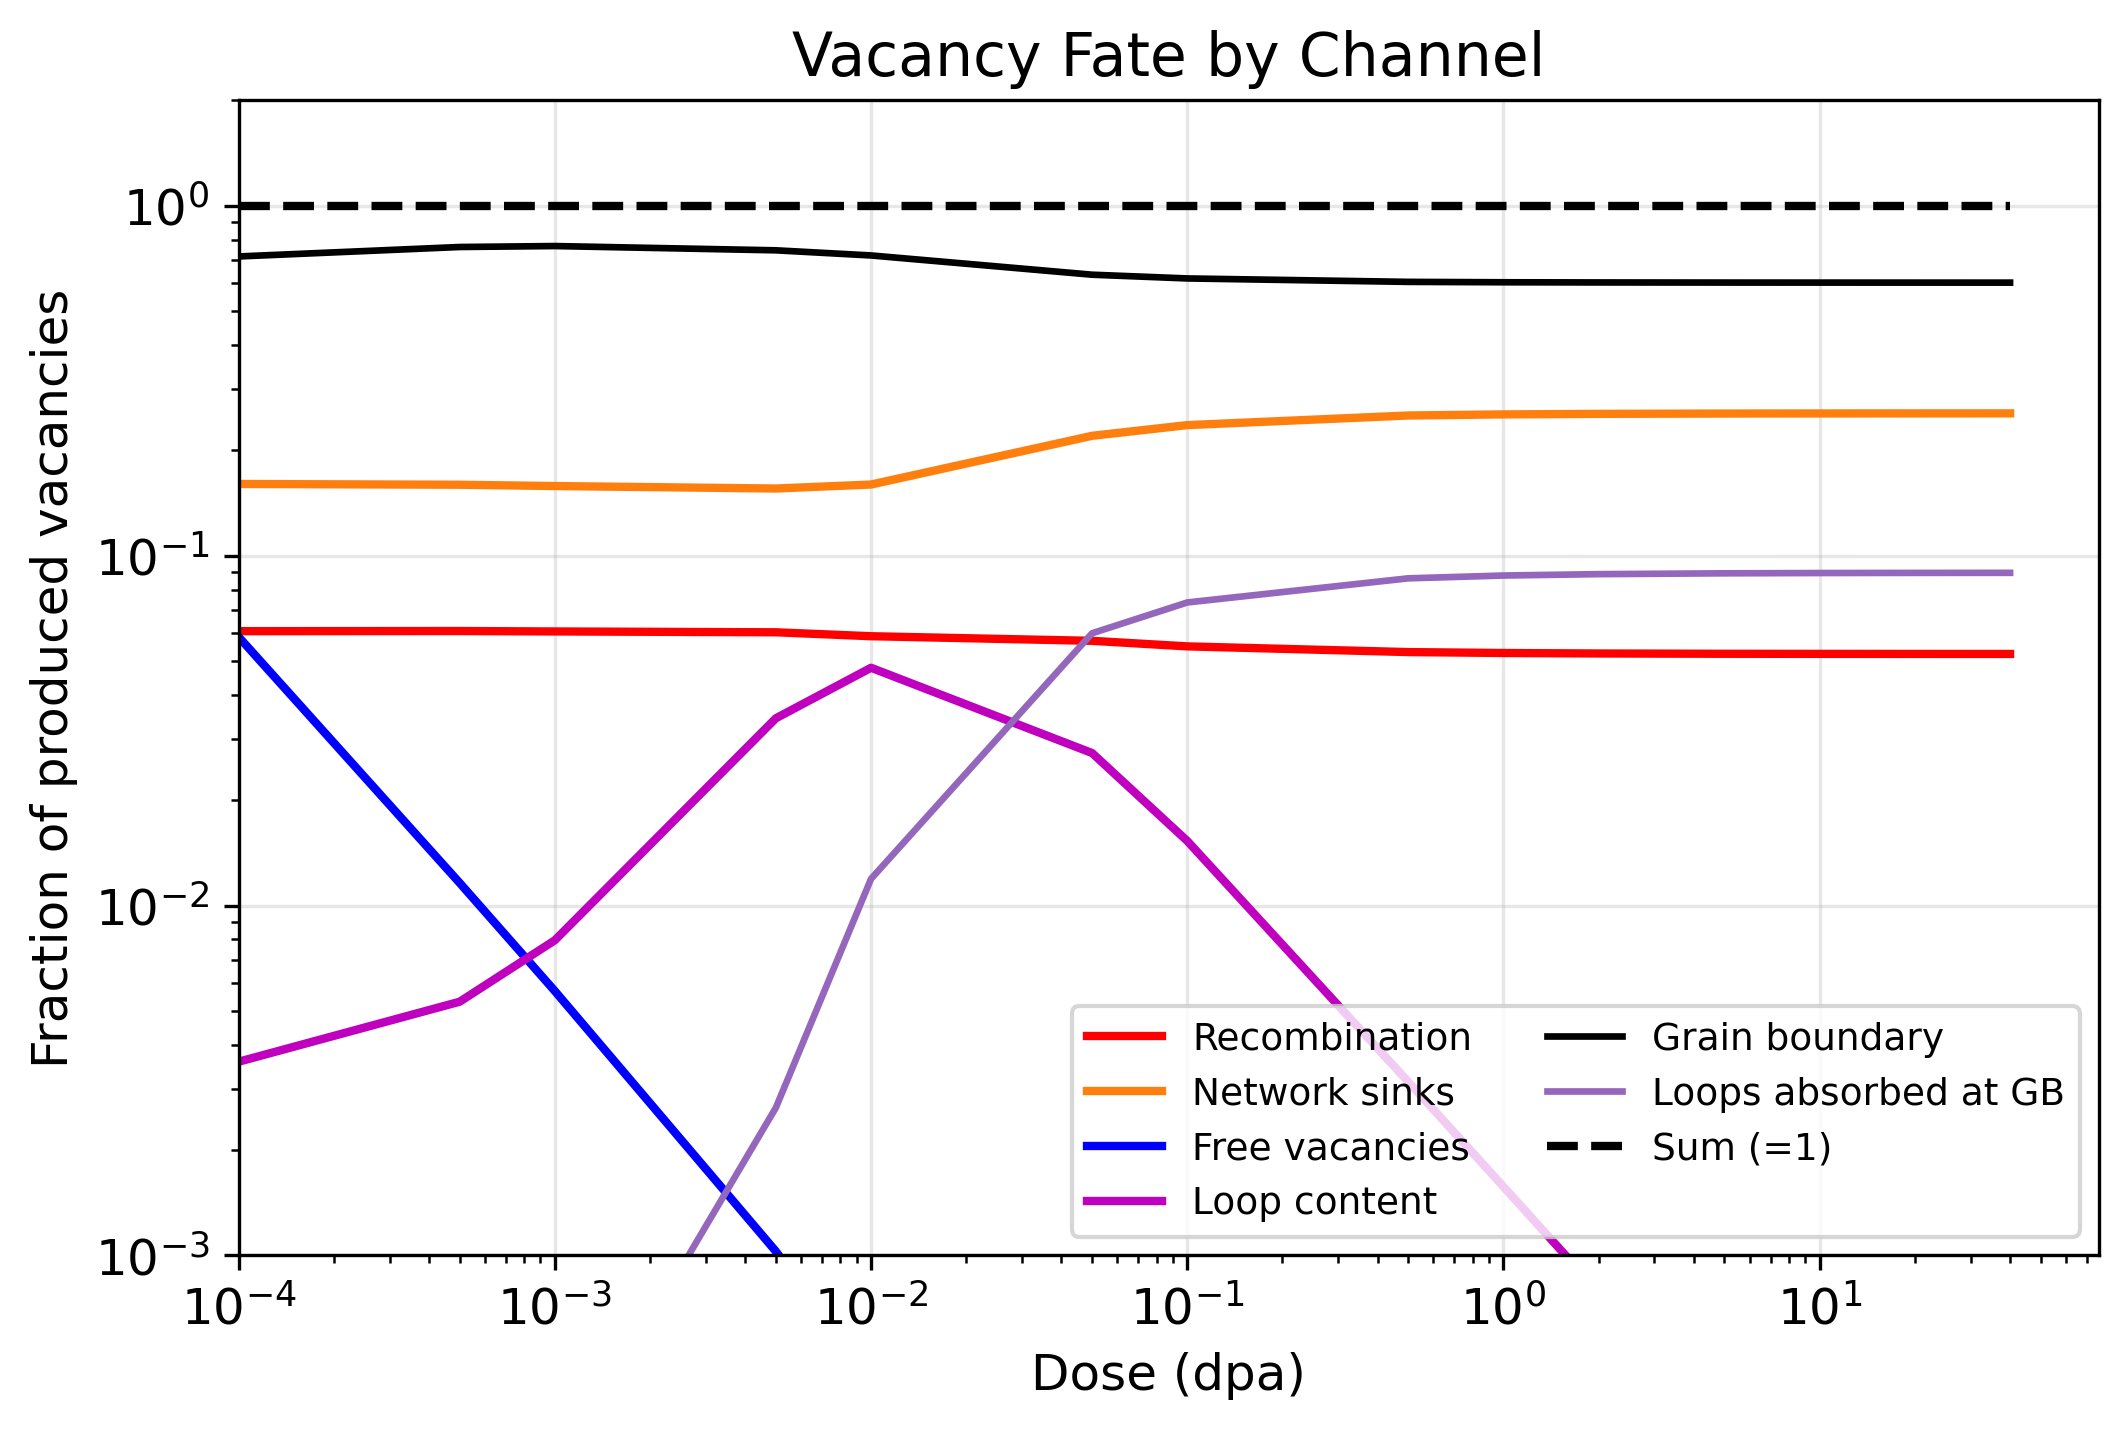
\includegraphics[width=\textwidth]{figures/fractions_v.png}
\end{minipage}
\caption{Vacancy balance against dose: cumulative channels (left) and their
fractions of production (right). The interstitial counterparts are similar
except that the loop-at-boundary channel is 60 times smaller.}
\label{fig:conservation}
\end{figure}

\begin{figure}[htbp]
\centering
\begin{minipage}{0.49\textwidth}\centering
  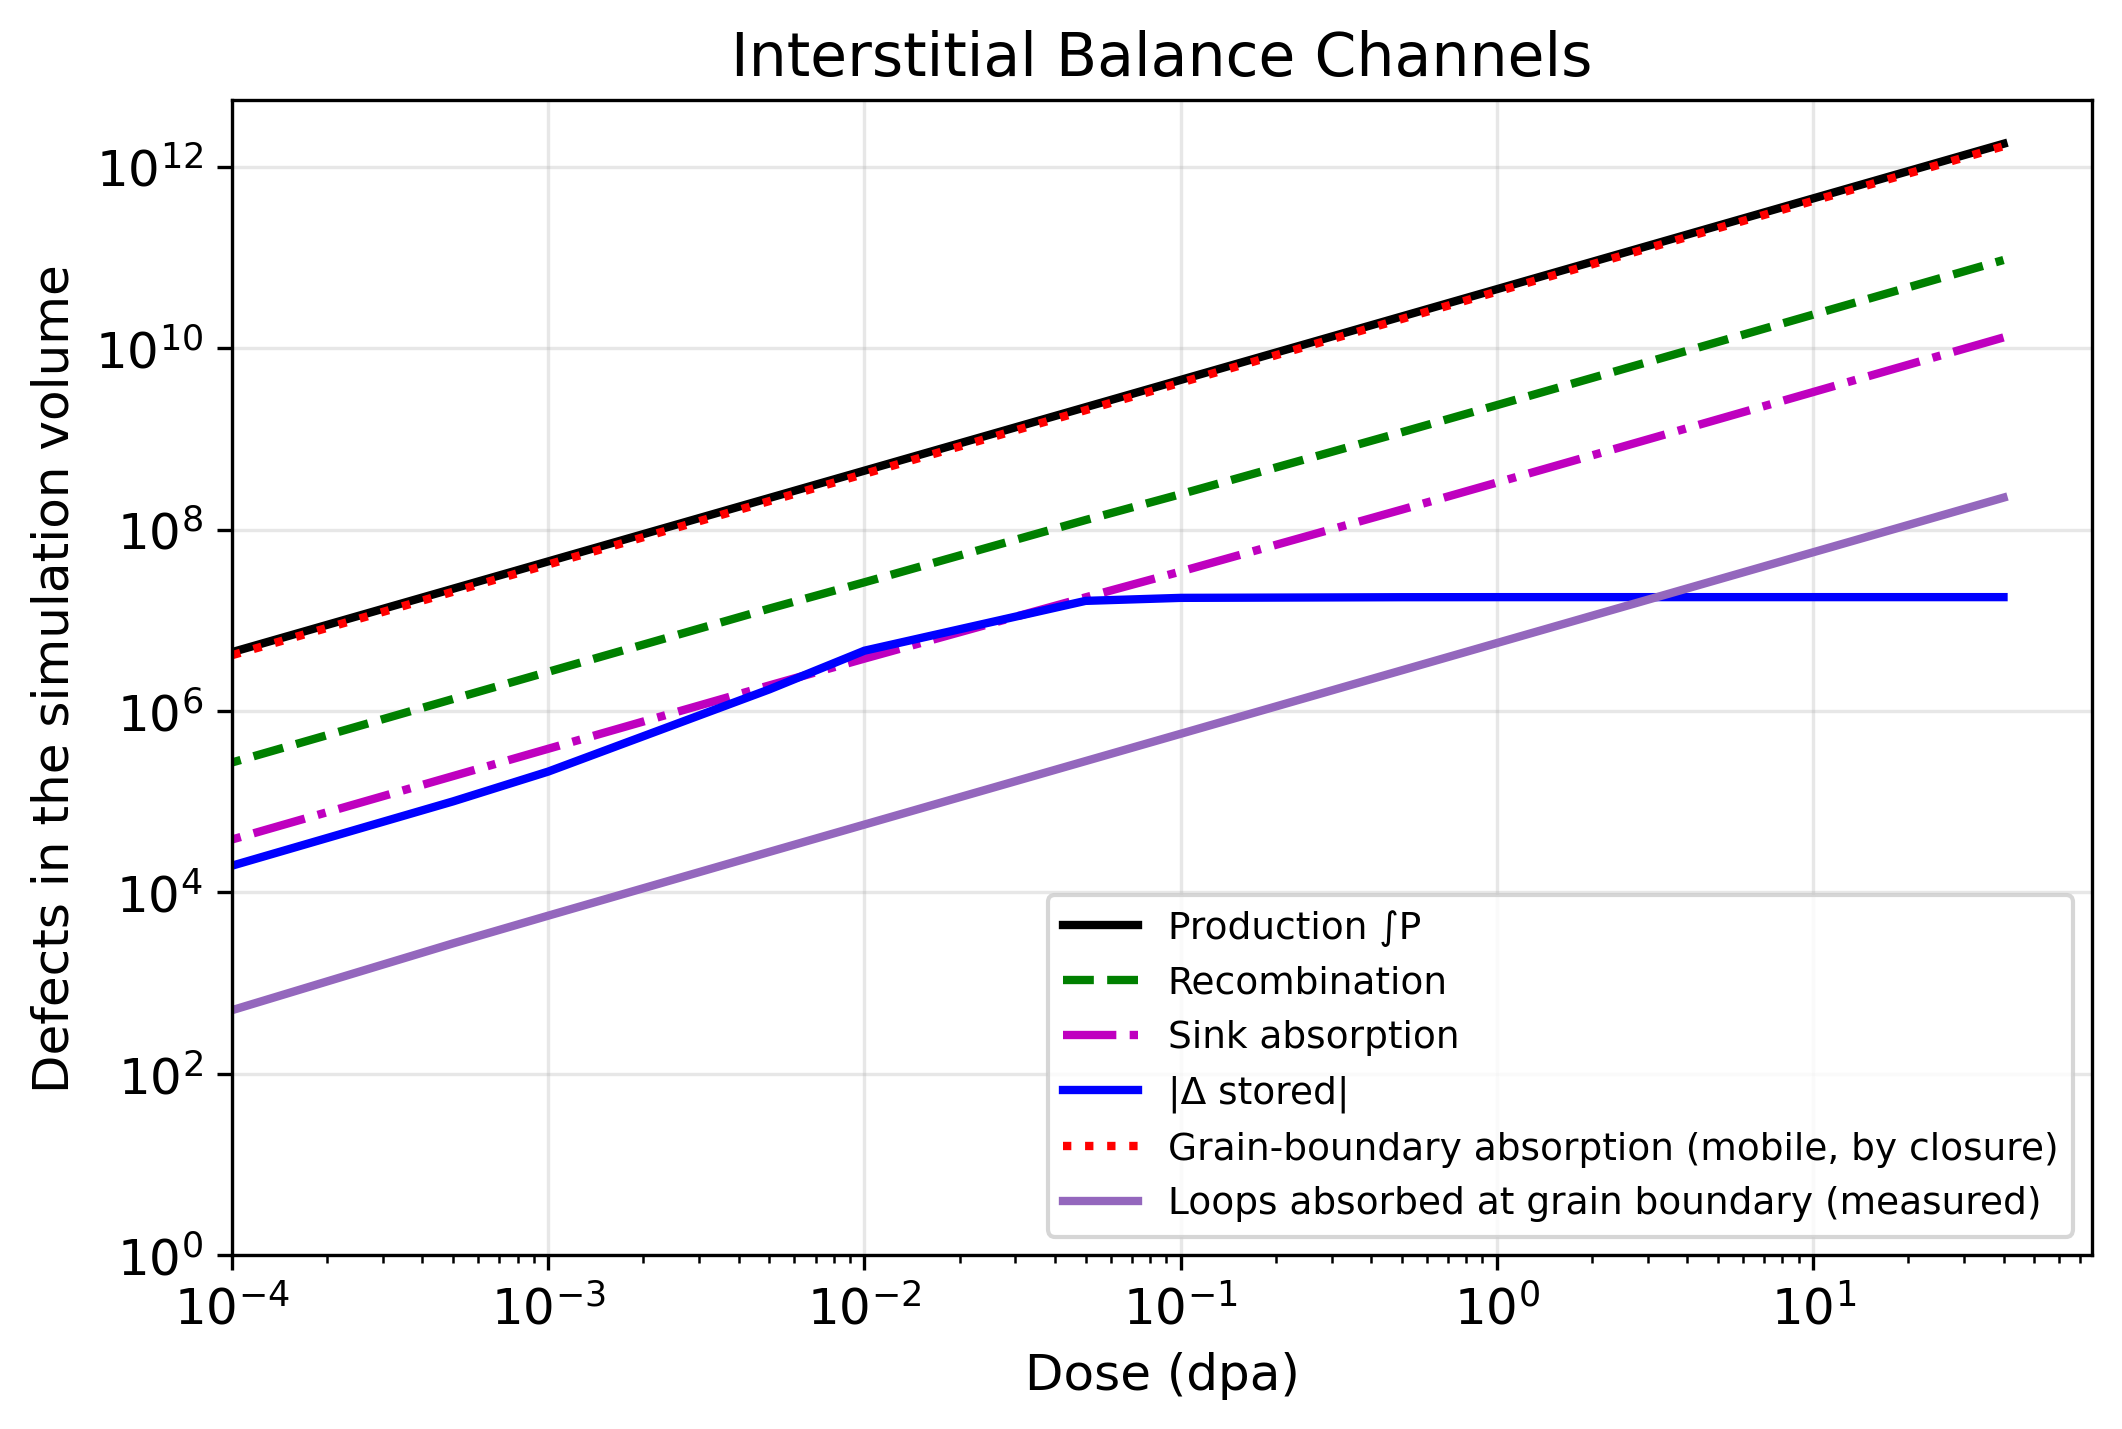
\includegraphics[width=\textwidth]{figures/conservation_i.png}
\end{minipage}\hfill
\begin{minipage}{0.49\textwidth}\centering
  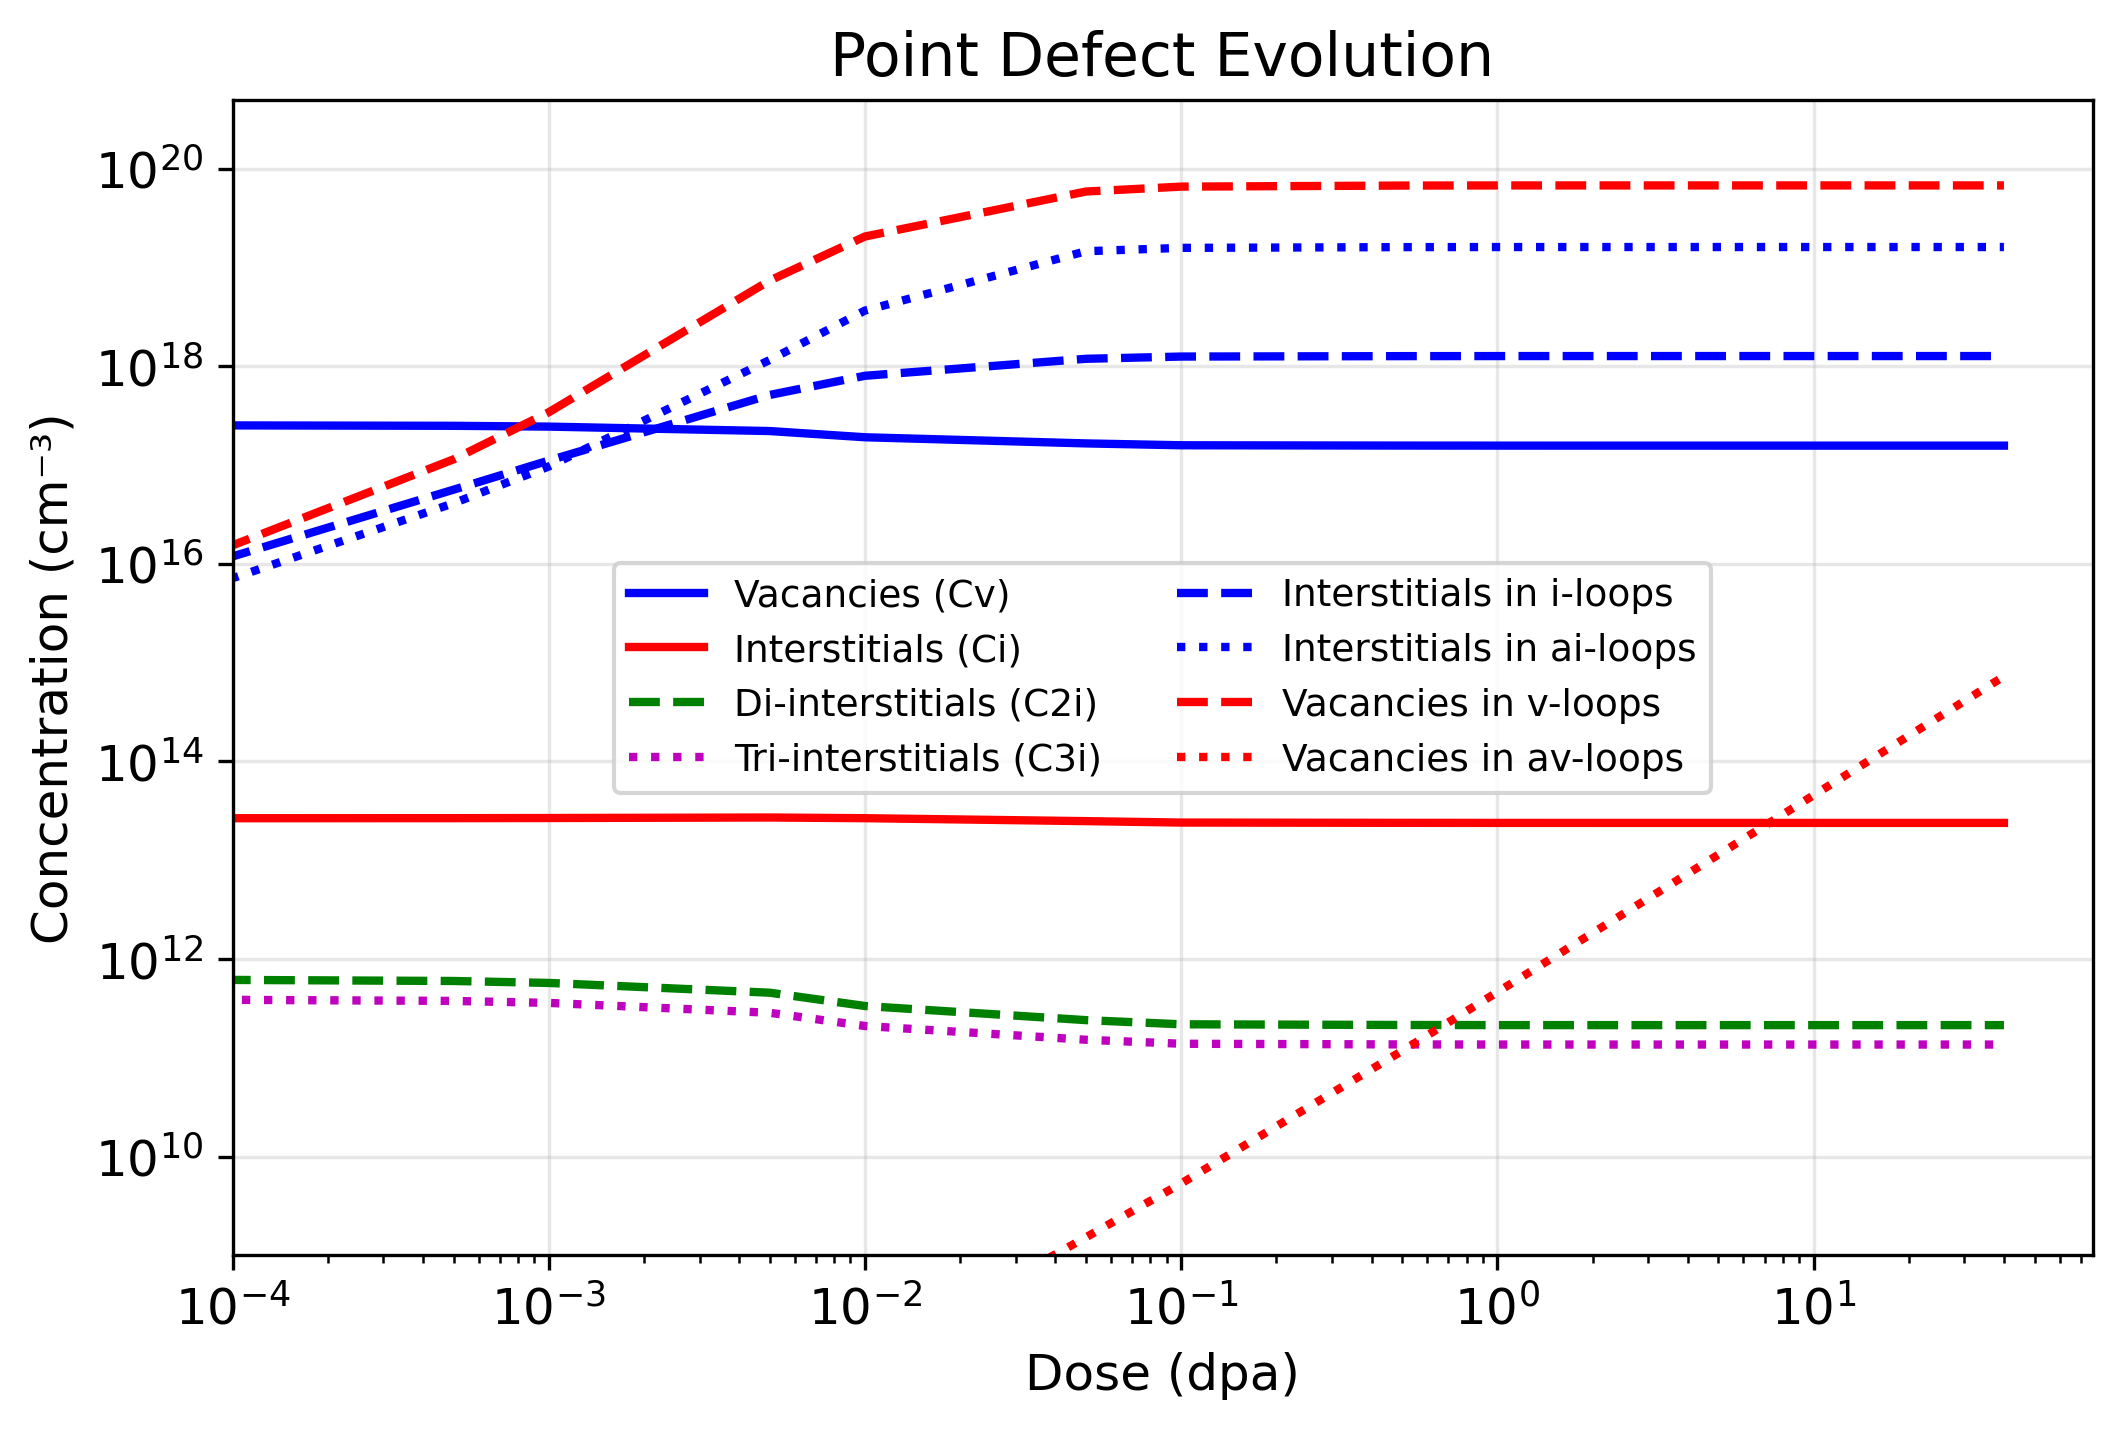
\includegraphics[width=\textwidth]{figures/point_defects.png}
\end{minipage}
\caption{Left: the interstitial balance against dose, the counterpart of
\cref{fig:conservation}. Right: the volume-averaged mobile concentrations, whose
fall through the march is the rising sink density of
\cref{sec:results-mobile} seen as an average rather than as a field.}
\label{fig:conservation-i}
\end{figure}

\subsection{Grain-boundary effects and the denuded zone}
\label{sec:results-gb}

\Cref{fig:denuded} is the central result of the loop channel: loop density and
mean diameter against distance to the nearest face, with and without it.

\begin{figure}[htbp]
\centering
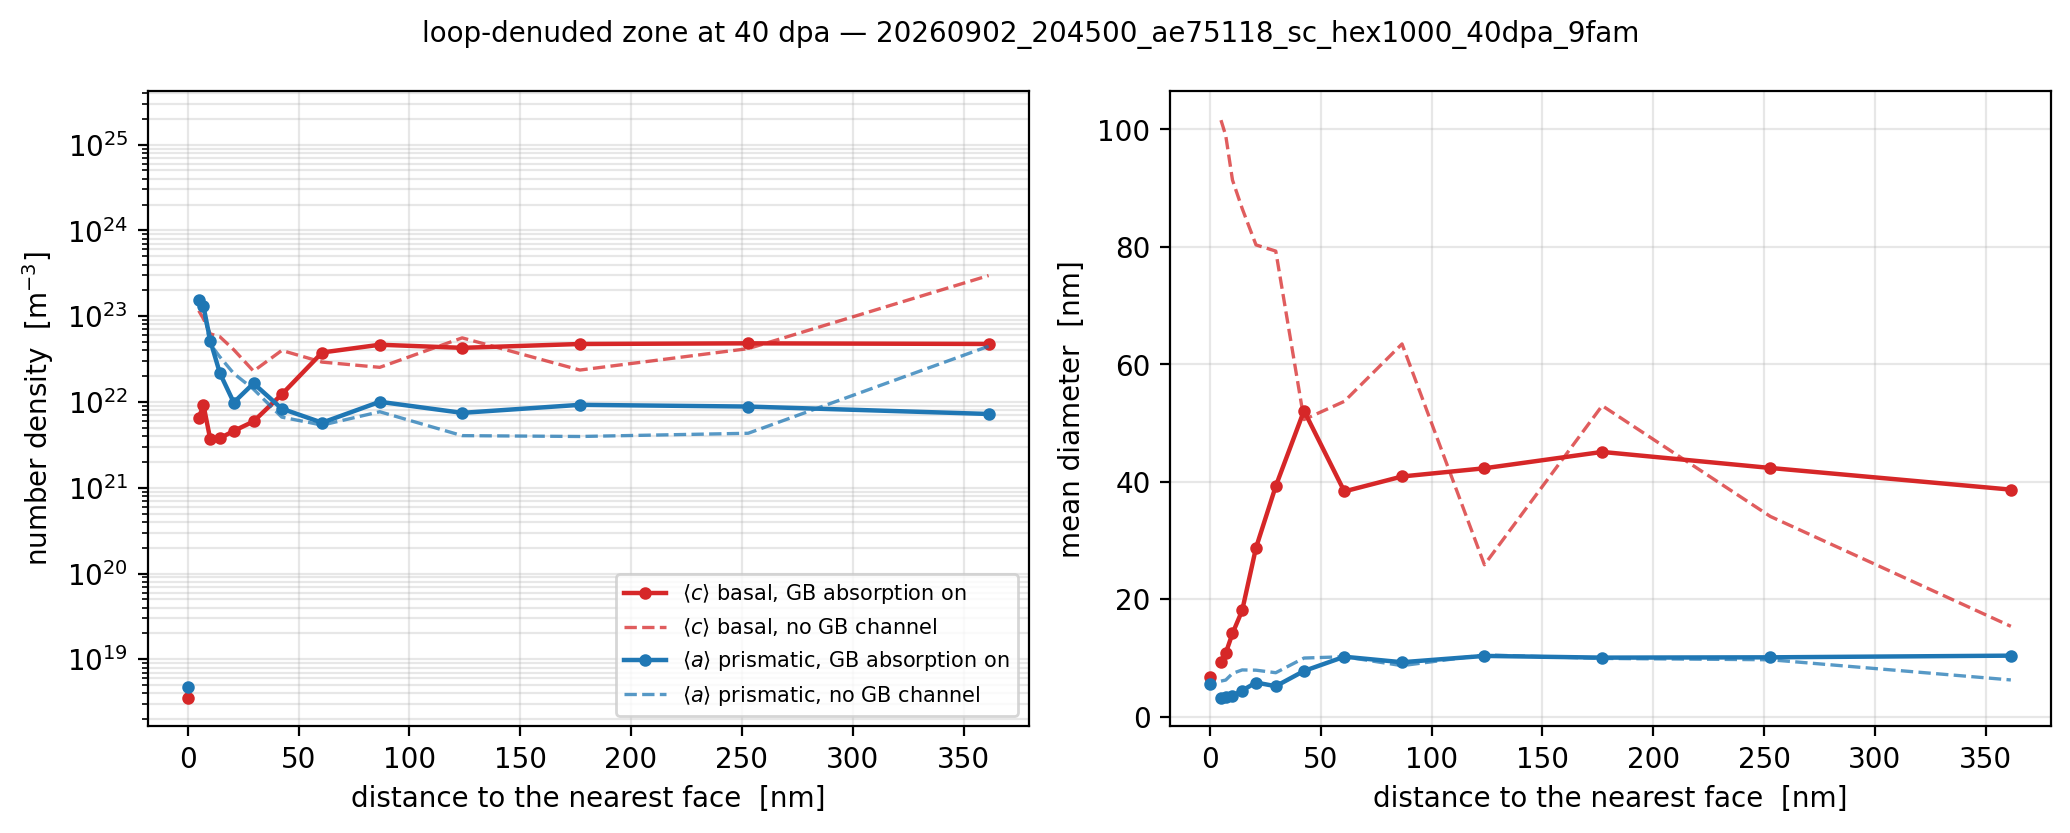
\includegraphics[width=\textwidth]{figures/denuded_zone.png}
\caption{The loop-denuded zone at 10\,dpa. Solid: grain-boundary loop absorption
active. Dashed: the identical calculation without it. Left, number density;
right, content-weighted mean diameter. The abscissa is the minimum distance to
any face, and the ordinate on the left is logarithmic over six decades.}
\label{fig:denuded}
\end{figure}

\begin{center}
\begin{tabular}{@{}lrrrr@{}}
\toprule
$x$ (nm) & $N_a$/twin & $N_c$/twin & $d_a$ (nm) & $d_c$ (nm) \\
\midrule
0--1        & $10^{-6}$ & $10^{-6}$ & 5.0 & 5.4 \\
3.5--4.9    & 0.646 & 0.608 & 4.6 & 3.5 \\
6.7--9.1    & 0.703 & 1.36  & 7.1 & 10.1 \\
23.6--32.3  & 2.95  & 5.45  & 5.7 & 32.5 \\
83.3--114.3 & 0.415 & 4.21  & 9.2 & 50.2 \\
156.8--215  & 0.670 & 12.6  & 8.9 & 57.9 \\
\bottomrule
\end{tabular}
\end{center}

\textbf{The zone is real, sharp, and about 5\,nm wide.} The face layer is swept
to $10^{-6}$ of the companion calculation --- which is the concentration floor,
so as complete a removal as this model can express --- and the depletion is still
measurable at 5--9\,nm. Beyond that the profile is no longer denuded. The mean
diameter recovers monotonically from $3.5\,$nm at the boundary to $58\,$nm in
the interior, which is the size gradient a denuded zone is identified by in a
micrograph: not merely fewer loops near the boundary, but \emph{smaller} ones,
because the large end of the distribution is what \cref{eq:gbloop} removes first.

\textbf{The ledger and the density profile measure different things, and both
are correct.} Of the total absorption, only 1.7\% occurs within 2\,nm of a face
and 93\% between 5 and 100\,nm. That is not a contradiction of the profile
above: the face layer is swept within the first dose interval, so for 99\% of the
march there is nothing left there to absorb, while the region further in keeps
\emph{supplying} loops that grow into contact. The density says where loops are
absent; the ledger says where the flux into the boundary came from over the whole
history.

\textbf{A local channel with non-local consequences.} The interior \cloop{}
density is 4--5 times the companion calculation's at \emph{every} distance,
including 200\,nm from any face where \cref{eq:mgb} removes nothing. The cause
is the operator split working as intended: removing the shell's loops removes
their sink strength from \cref{eq:KL}, the fast solve returns a different mobile
field everywhere, and the interior responds to it. A model in which the boundary
were only a mean-field sink strength could not produce this, because the
boundary's effect on the interior would be a single number rather than a changed
field.

\paragraph{Comparison with experiment.} Loop-denuded and void-denuded zones at
grain boundaries are a standard observation in irradiated
metals~\citep{singh1973influence,bai2010efficient,sun2013situ,cheng2016grain}, and the mechanism
assumed here --- the boundary as a strong sink whose influence extends a
diffusion length into the grain --- is the standard interpretation. \textbf{We
do not compare quantitatively against a measured zone width in zirconium}: no
such measurement is in the data set of \cref{tab:targets}, and the width
predicted here (a few nm for \aloop{}, growing to tens of nm in the size
profile) is offered as a prediction rather than as a validated result. It is
also, at $2$--$5\,$nm for the prismatic family, comparable with the $20\,$nm
element size of the boundary layer, so the \aloop{} zone in particular is
under-resolved and its width should be treated as an upper bound set by the
mesh.

\begin{figure}[htbp]
\centering
\begin{minipage}{0.49\textwidth}\centering
  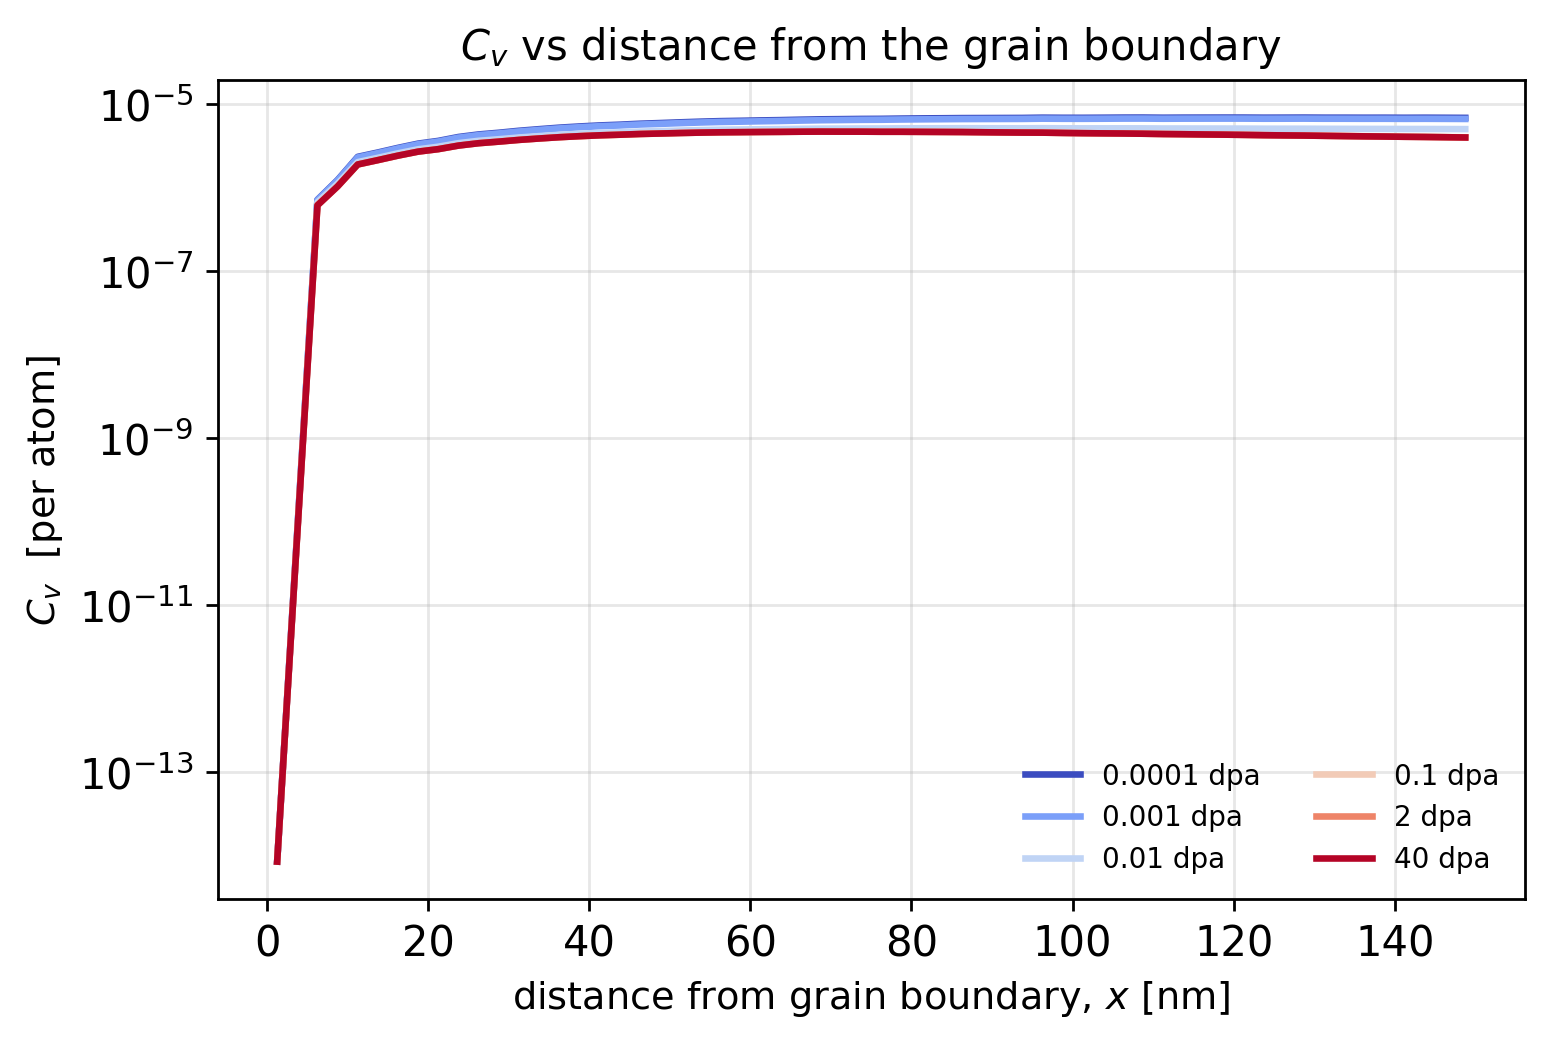
\includegraphics[width=\textwidth]{figures/gb_Cv.png}
\end{minipage}\hfill
\begin{minipage}{0.49\textwidth}\centering
  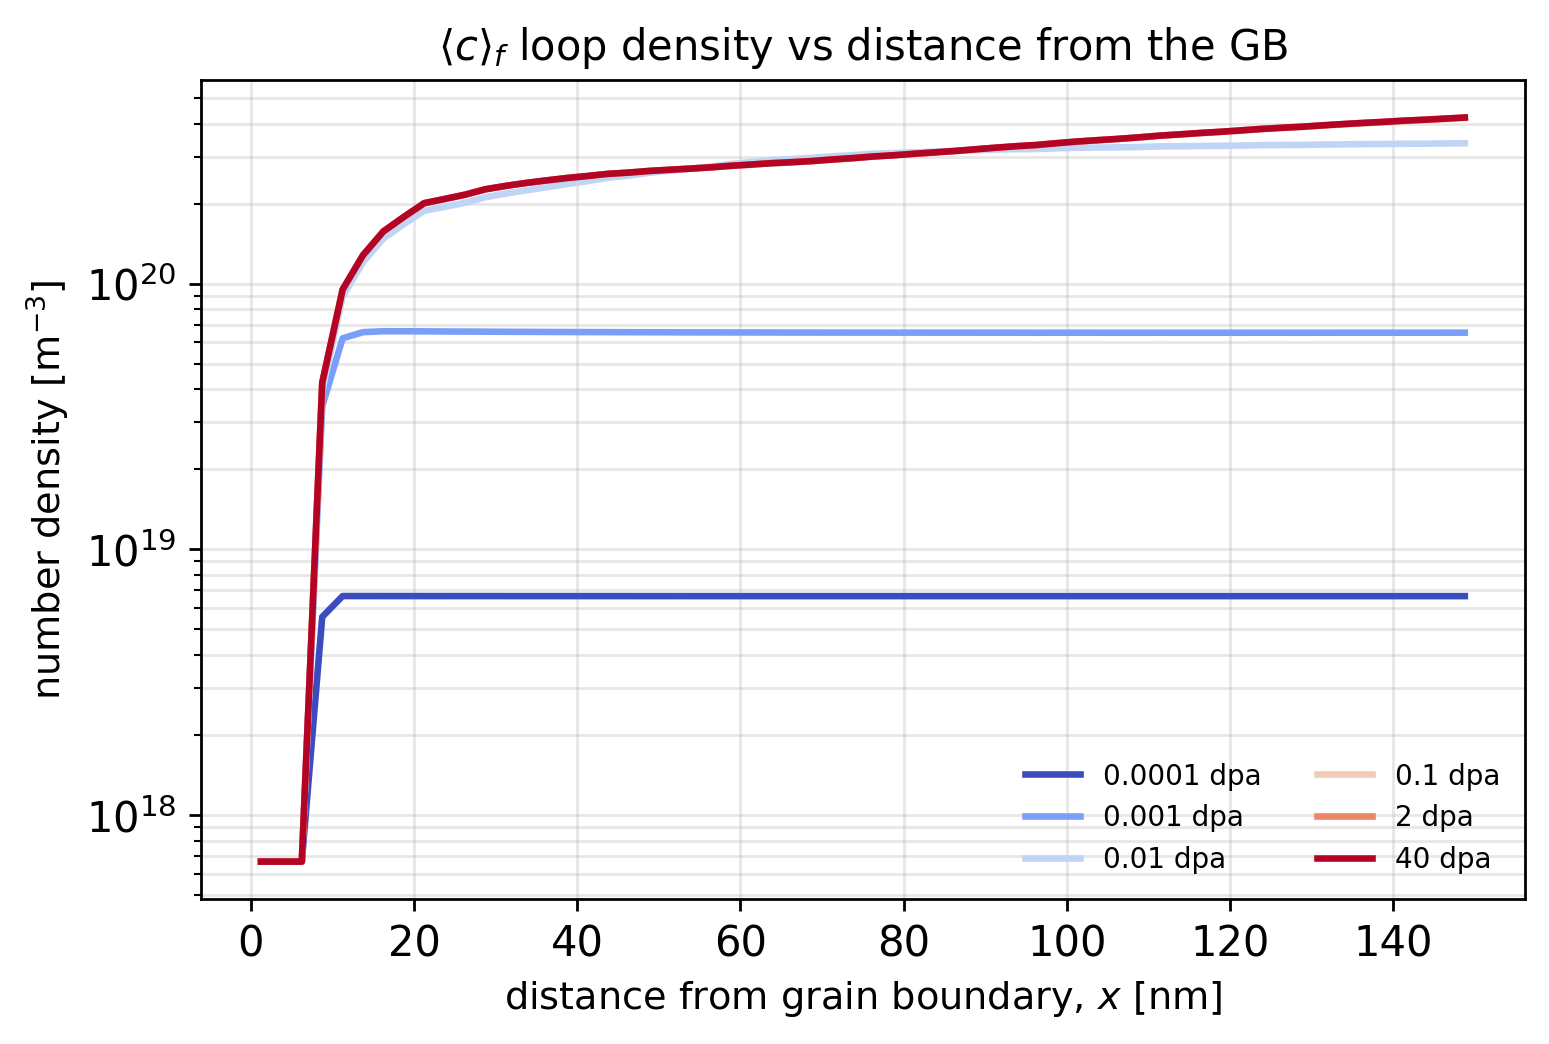
\includegraphics[width=\textwidth]{figures/gb_N_c.png}
\end{minipage}
\caption{Profiles against distance from the boundary over the first
\SI{150}{\nano\meter}, with every dose overlaid. Left: the mobile vacancy
concentration, whose recovery length is the boundary layer tabulated above and
which narrows as the dose accumulates. Right: the basal \cloop{} loop number
density, whose profile is the denuded zone of \cref{fig:denuded} seen at every
dose rather than only at the last.}
\label{fig:gb-profiles}
\end{figure}

\subsection{Volume averages and comparison with experiment}
\label{sec:results-volume}

\Cref{fig:volavg} shows the volume-averaged trajectories.

\begin{figure}[htbp]
\centering
\begin{minipage}{0.49\textwidth}\centering
  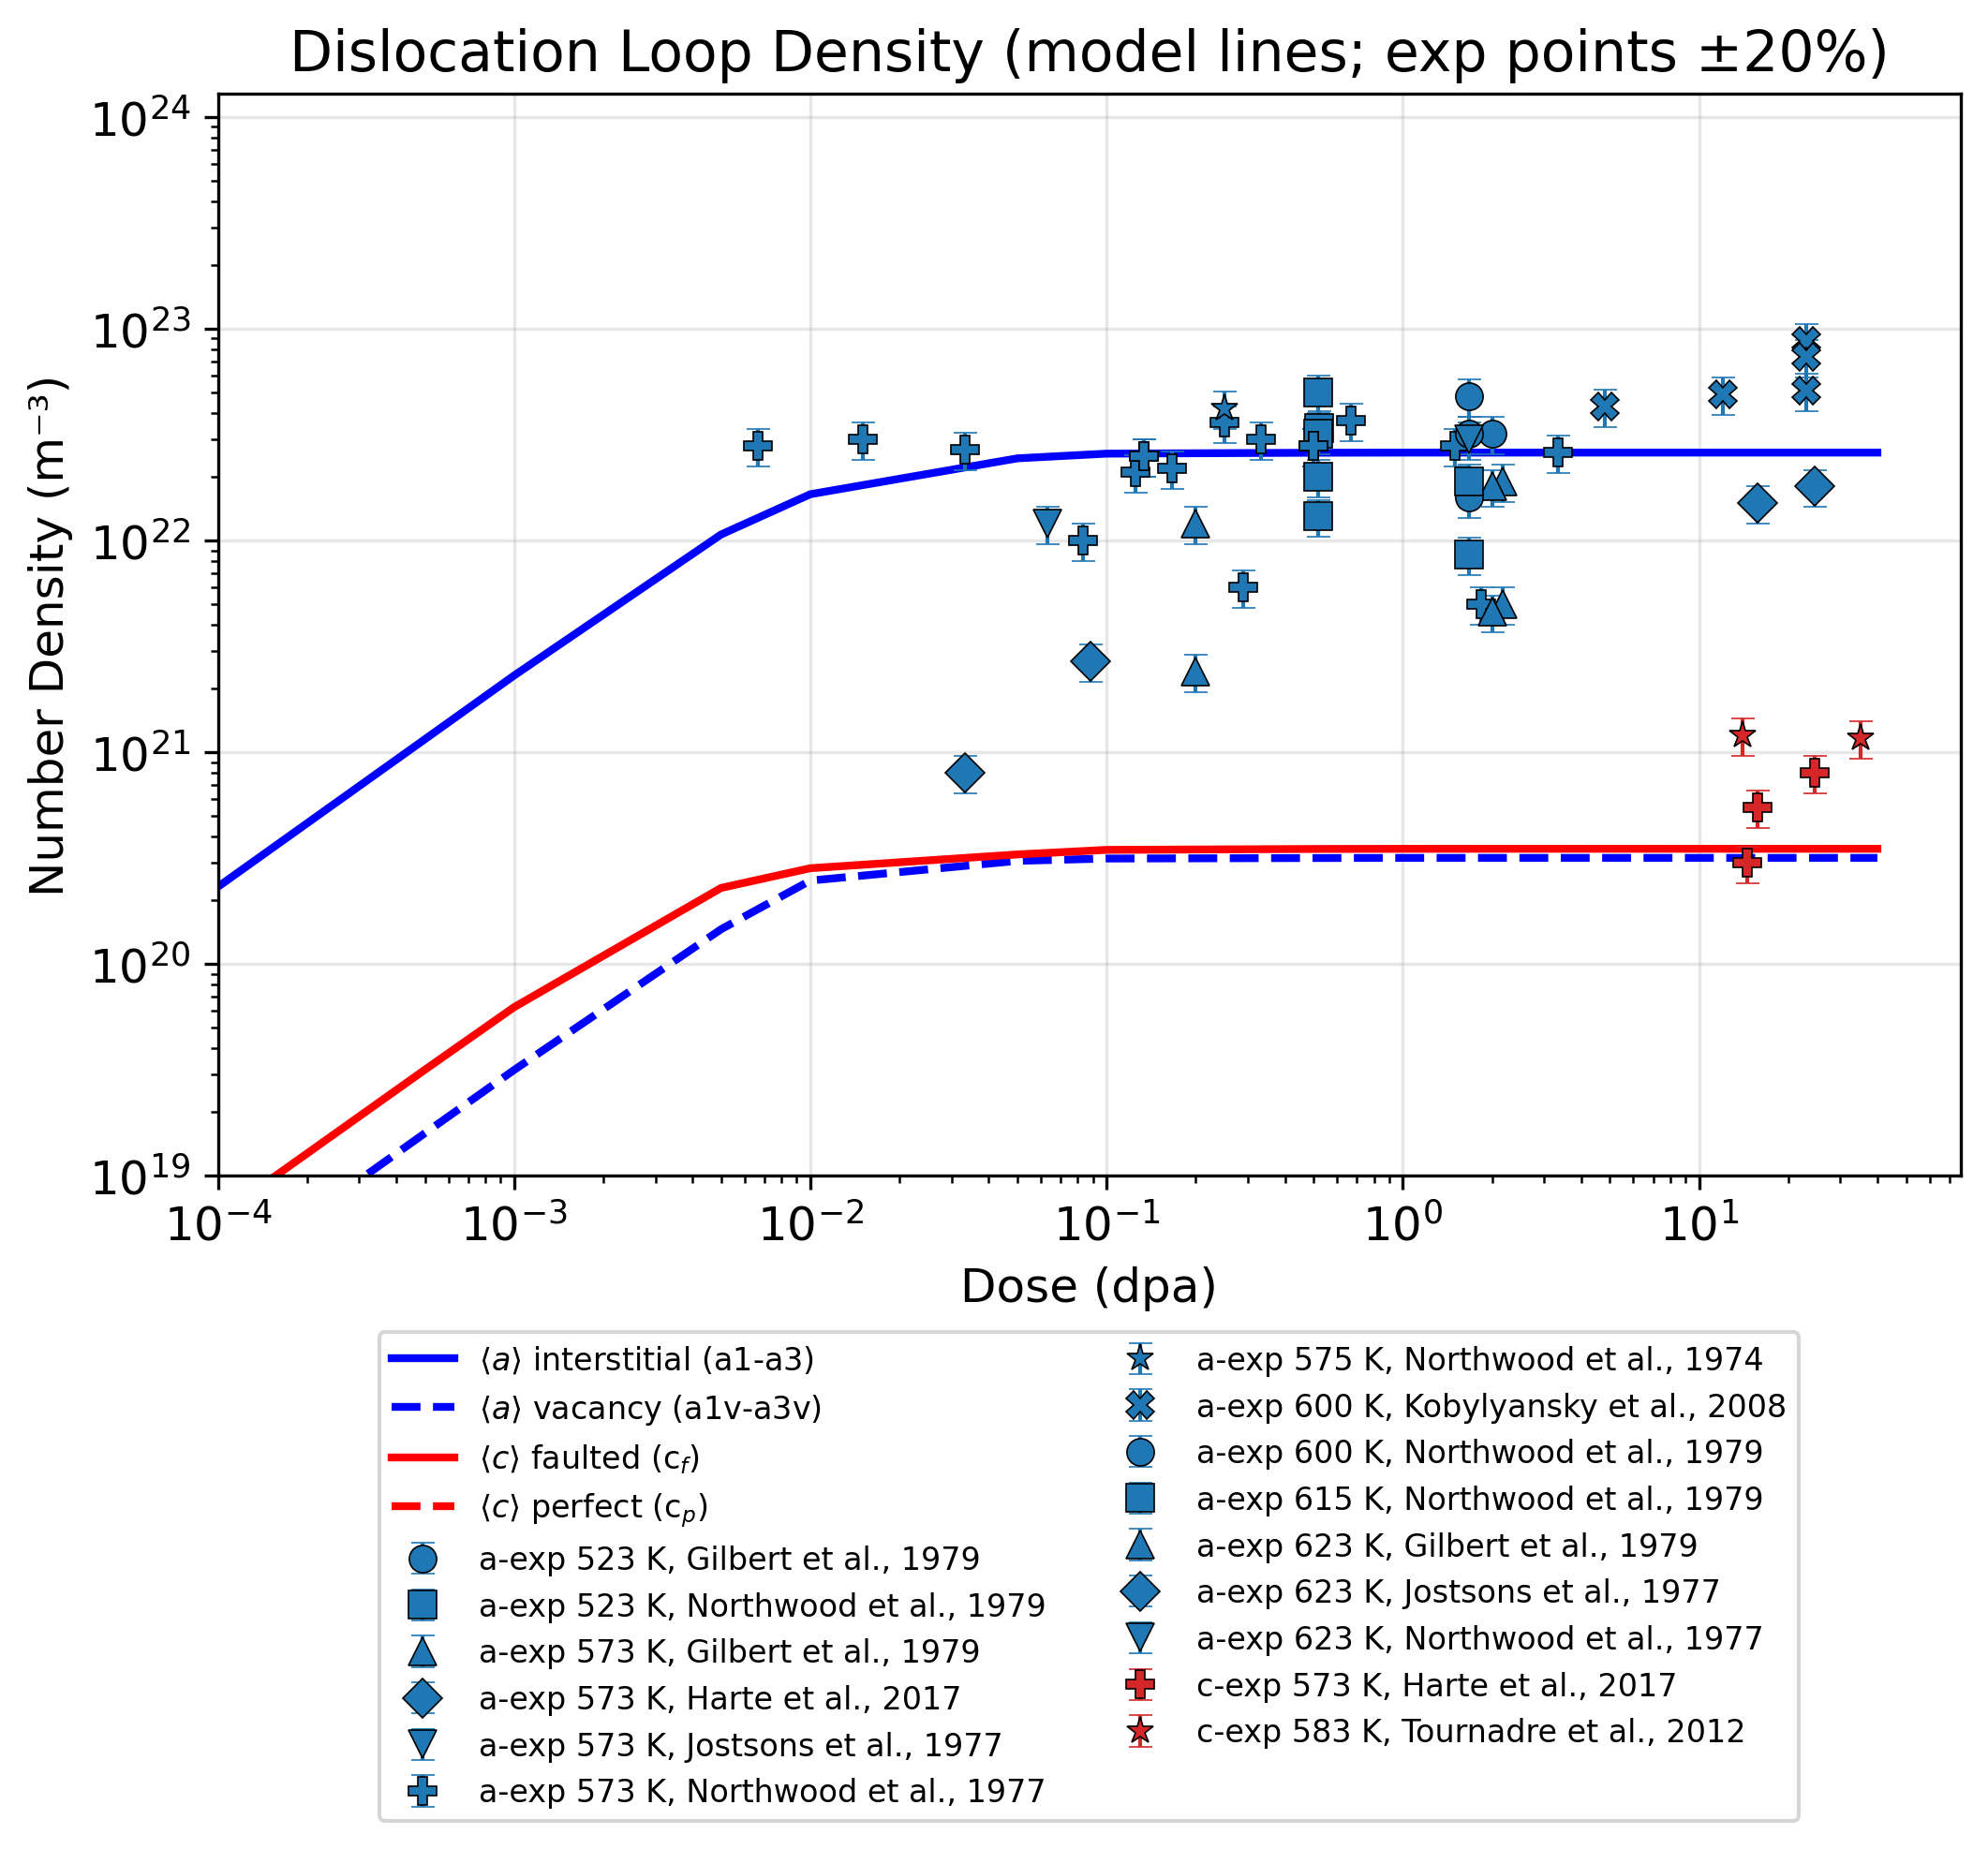
\includegraphics[width=\textwidth]{figures/loop_density.png}
\end{minipage}\hfill
\begin{minipage}{0.49\textwidth}\centering
  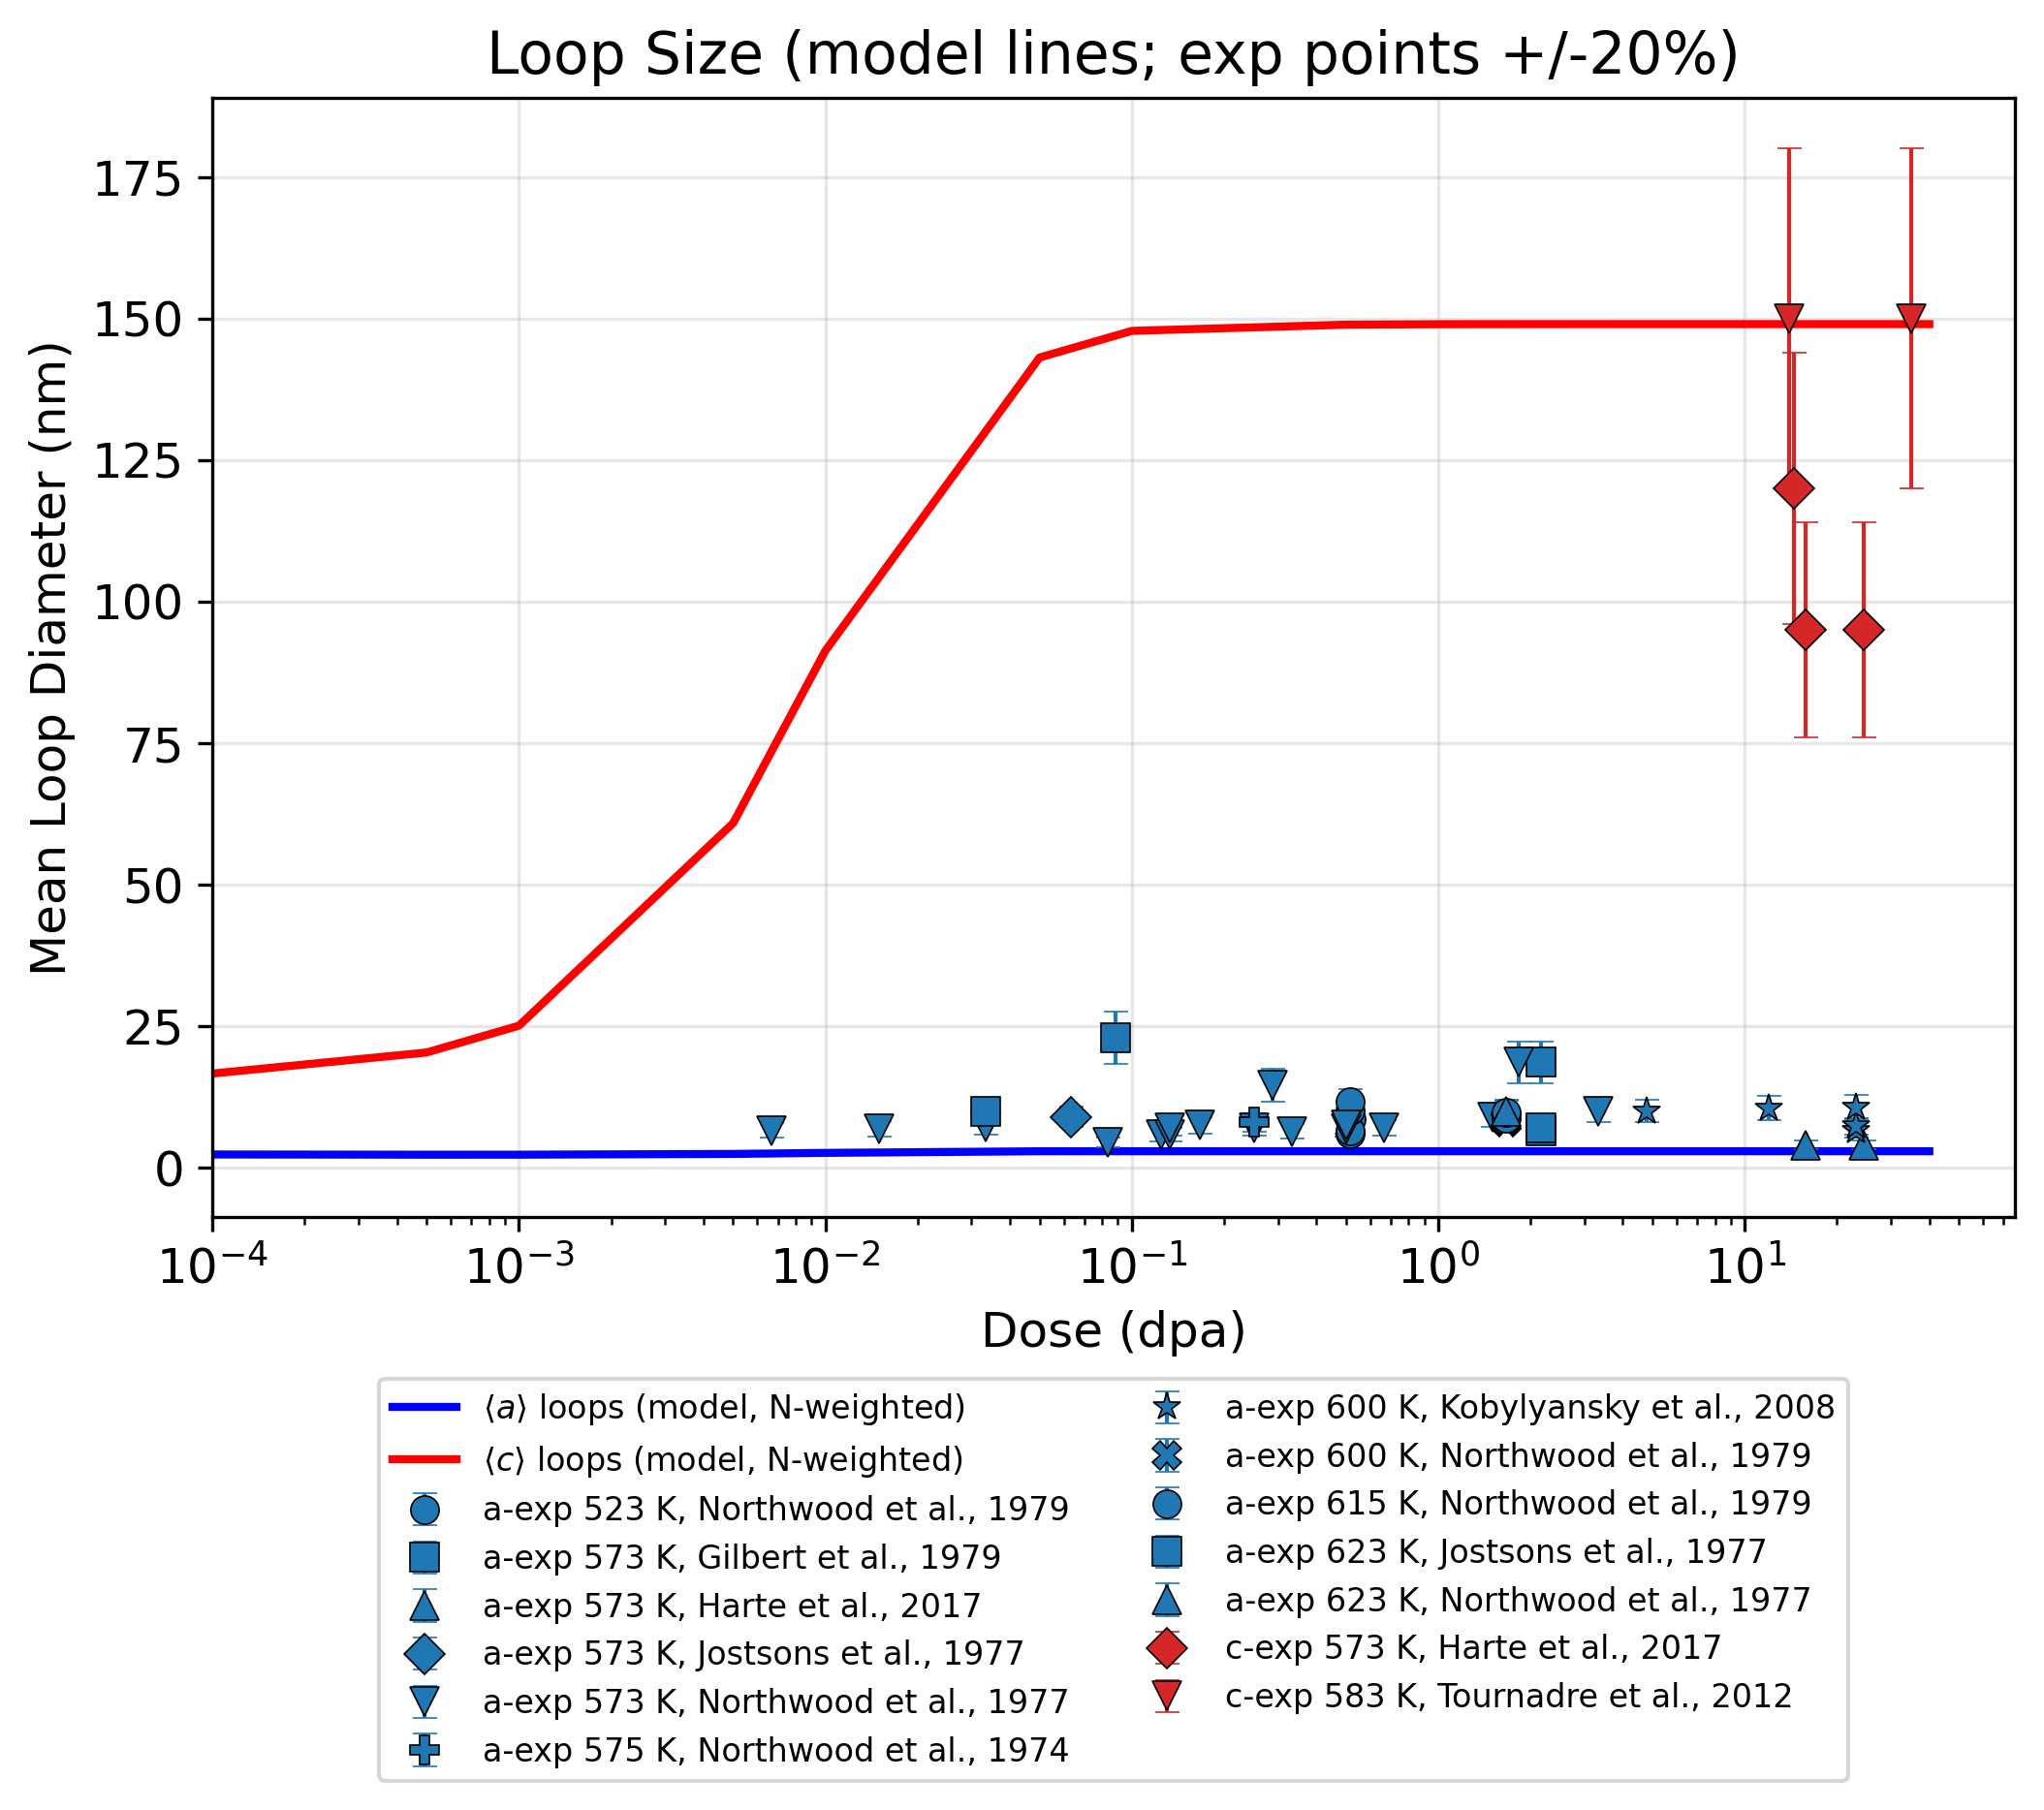
\includegraphics[width=\textwidth]{figures/loop_sizes_vs_exp.png}
\end{minipage}
\caption{Volume-averaged loop density against dose (left) and mean size against
the experimental measurements (right).}
\label{fig:volavg}
\end{figure}

\textbf{Which average is quoted is not a presentational choice.} On a Dirichlet
domain the boundary shell is a sink for mobile defects and --- without the
channel of \cref{sec:gb-loops} --- not a sink for loops, so it accumulates a
loop population that is numerous, tiny, and entirely unphysical as a description
of the material. At 10\,dpa:

\begin{center}
\begin{tabular}{@{}llrrrr@{}}
\toprule
& Region & $N_a$ (m$^{-3}$) & $d_a$ (nm) & $N_c$ (m$^{-3}$) & $d_c$ (nm) \\
\midrule
\multirow{2}{*}{loop channel off}
 & domain   & $1.32\times10^{24}$ & 5.01 & $1.41\times10^{24}$ & 5.74 \\
 & interior & $6.06\times10^{21}$ & 5.93 & $1.62\times10^{21}$ & 70.16 \\
\midrule
\multirow{2}{*}{loop channel on}
 & domain   & $4.61\times10^{21}$ & 7.41 & $6.74\times10^{21}$ & 37.07 \\
 & interior & $2.90\times10^{21}$ & 9.16 & $7.64\times10^{21}$ & 50.62 \\
\bottomrule
\end{tabular}
\end{center}

Without the channel the domain and interior means differ by a factor of $217$ in
$N_a$ and $873$ in $N_c$, and the domain-mean diameter \emph{falls} to 5.7\,nm
while the interior mean grows to 70\,nm --- the domain average is measuring the
boundary shell and nothing else. \textbf{With the channel the two agree to
within a factor of 1.6}, and a domain average becomes a statement about the
material. That is the strongest single argument for carrying the channel: it
removes an artifact that otherwise makes the most natural summary statistic
meaningless.

\paragraph{Against experiment, and the discrepancy.} At $573\,$K and 24.5\,dpa
the measurements give $N_c=8.0\times10^{20}\,\mathrm{m^{-3}}$ and
$d_c=95\,$nm. The interior of this calculation at 10\,dpa gives
$N_c/N^{\exp}=9.5$ and $d_c/d^{\exp}=0.53$: \textbf{too many loops, and too
small}. The companion without the loop channel gives $2.0$ and $0.74$ --- closer
on both, which is expected and is not an argument against the channel: the
parameters of \cref{tab:fitted} were fitted in a $0$-D that has no boundary at
all (\cref{sec:bias-caveat}), so the channel is an unmodeled loss acting on a
population calibrated without it. A refit with the channel active is required
before either number is quoted as a prediction.

The direction of the discrepancy is the informative part, and it is the same one
the calibration reported. The model produces \emph{more, smaller} \cloop{} loops
than are observed, and the two errors are linked: the number balance pins the
total content while the growth balance pins the size, so density is their
quotient and a model that removes loops faster than it grows them necessarily
has survivors that are too young. What the data want is \emph{fewer and larger},
and no channel exercised here achieves both. \Cref{sec:conclusions} states what
this implies.

\subsection{Continuum-to-discrete conversion}
\label{sec:results-discrete}

The conversion of \cref{sec:transfer} was applied to the fields at four doses.
The number of loops is not a parameter of the conversion: it is
$\sum_j n_j V_j$, the number the field says is present.

\begin{center}
\begin{tabular}{@{}lrrrr@{}}
\toprule
Family & $10^{-4}$\,dpa & $10^{-2}$\,dpa & 1\,dpa & 10\,dpa \\
\midrule
$c_f$ (basal, vacancy)          & 9 & 858 & 1031 & 1073 \\
$a_1$ (prismatic, interstitial) & 2 & 132 &   67 &   73 \\
$a_1^{v}$ (prismatic, vacancy)  & 2 &  87 &   56 &   61 \\
\bottomrule
\end{tabular}
\end{center}

\Cref{fig:discrete} shows the basal population at those four doses, drawn at
true radius and true position, over the continuum content field it was drawn
from. The two representations agree loop for loop: the figure is built from the
same draw the conversion exports, so a reader comparing this figure with the
exported loop table is comparing one object with itself.

\begin{figure}[htbp]
\centering
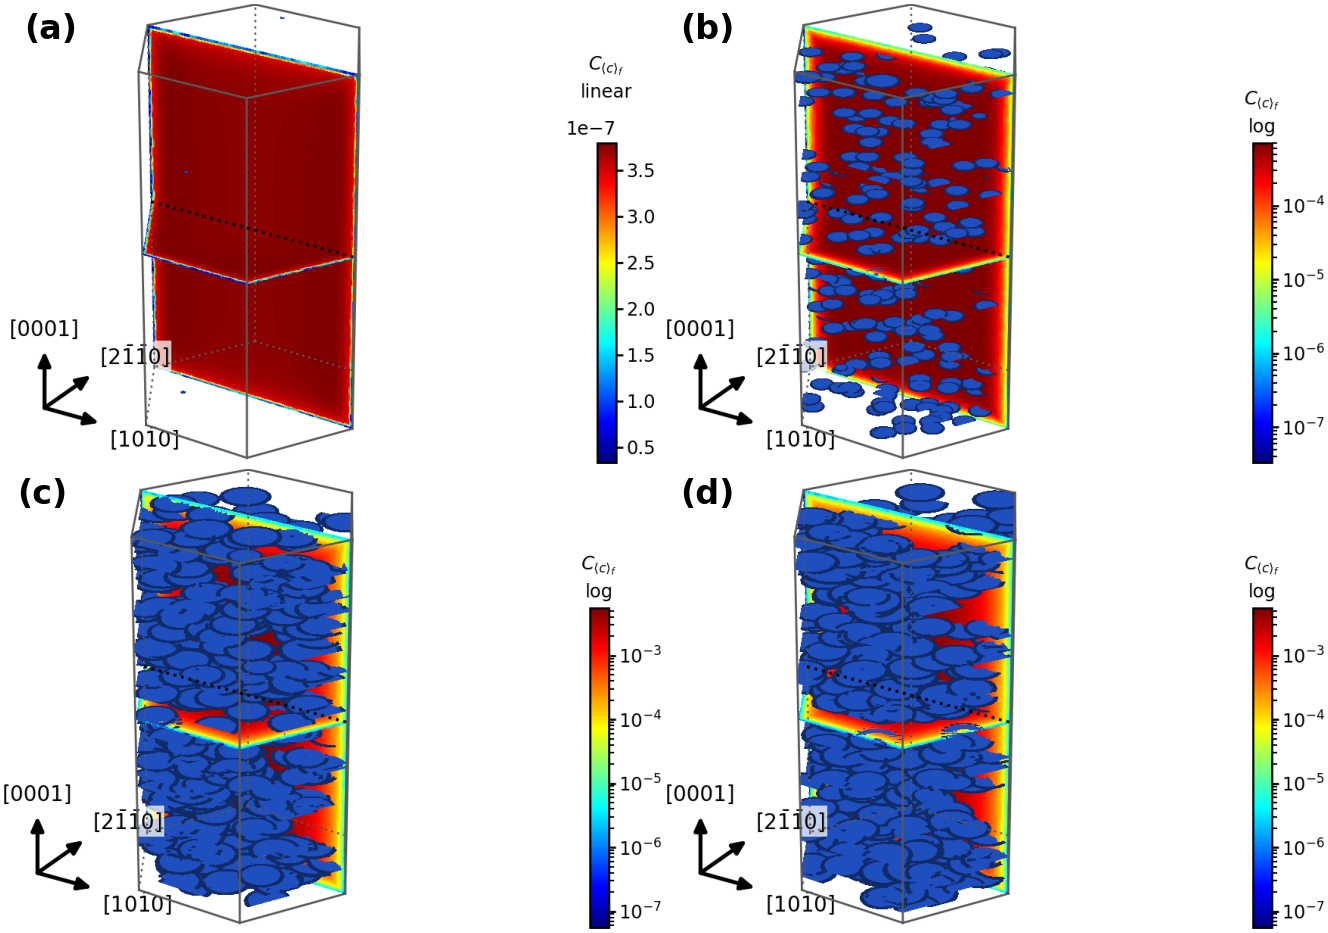
\includegraphics[width=\textwidth]{figures/loops_c_4dose.png}
\caption{The discrete basal \cloop{} population at (a) $10^{-4}$, (b) $10^{-2}$,
(c) 1 and (d) 10\,dpa, drawn at true radius over the continuum content field.
Counts are 9, 858, 1031 and 1073. The loops are clipped at the crystal surface;
see the text.}
\label{fig:discrete}
\end{figure}

\begin{figure}[htbp]
\centering
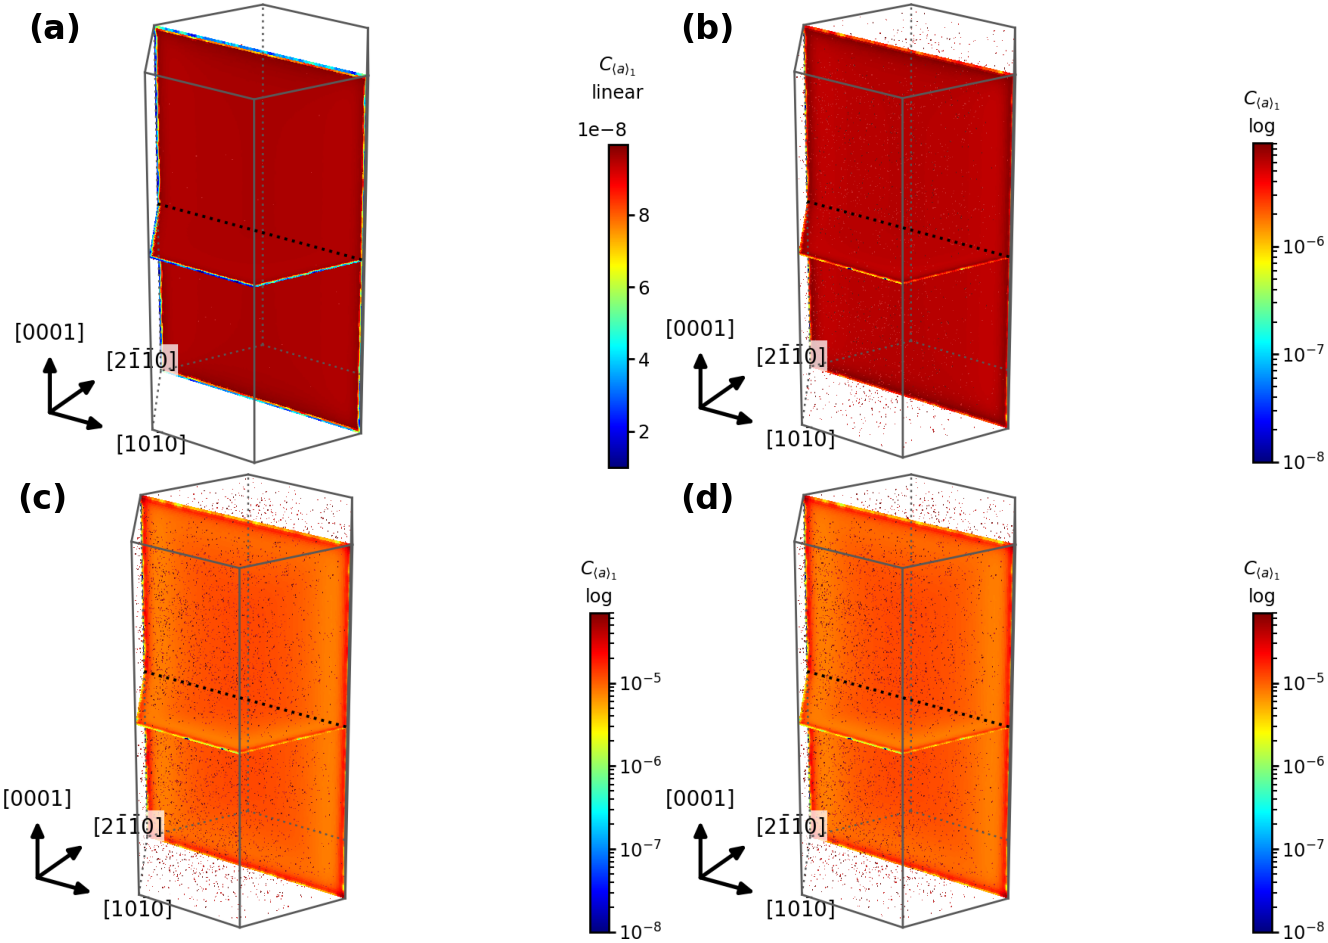
\includegraphics[width=\textwidth]{figures/loops_a1_4dose.png}
\caption{The discrete prismatic \aloop{}$_1$ population at the same four doses,
(a) $10^{-4}$, (b) $10^{-2}$, (c) 1 and (d) 10\,dpa, drawn at true radius.
Counts are 2, 132, 67 and 73. At true scale these loops are $6$--$7$\,nm across
in a \SI{500}{\nano\meter} crystal and are correspondingly sparse; the same
population drawn with exaggerated radii is legible but is not a population.}
\label{fig:discrete-a}
\end{figure}

Three observations.

\textbf{The count is not monotone, and it should not be.} Between $10^{-2}$ and
1\,dpa the prismatic count \emph{halves}, from 132 to 67, while the stored
content rises. That is coalescence: loops merge, so fewer, larger loops hold more
content. A conversion that preserved number rather than content would have hidden
this.

\textbf{A quarter of the basal loops do not fit.} At 10\,dpa, 287 of 1073
\cloop{} loops (26.7\%) are centered within their own radius of a face and
overhang it, by up to 40\,nm; the corresponding prismatic figure is 8.2\%. The
drawn population is clipped at the surface, but the clip is a drawing convention
and the exported loops are whole. This is the same geometric refusal that
\cref{sec:transfer} describes, and it means the basal handoff on a 500\,nm grain
is only partially feasible above $\sim0.1\,$dpa: a discrete-dislocation solver
would decline those loops, and their defects would have to remain in the
continuum. \emph{The correction to the \cloop{} Burgers vector that made the two
representations agree made this worse}, not better, because it raised the basal
radius by $\sqrt2$ and a larger loop is harder to fit.

\textbf{The conversion is where the mean field is checked against itself.} At
$10^{-4}\,$dpa the population is 9 basal and 2 prismatic loops in
$1.3\times10^{8}\,\mathrm{nm^{3}}$ --- a population so dilute that a continuum
density describing it is a statement about an ensemble and not about this
crystal. At 10\,dpa the basal loops are 50\,nm across with a mean spacing of
about 50\,nm, which is the opposite regime, and it is the one in which the
Avrami kernels of \cref{eq:avrami} are working hardest and are least defensible.
The conversion spans both, and the ledger of \cref{eq:ledger} closes on stored
defects to machine precision and on loop number to the integer draw at every one
of the four doses.

\section{Discussion and Conclusions}\label{sec:conclusions}

Self-consistency in sense~(a) is achievable and is a constraint worth accepting.
Every capture efficiency in \cref{eq:Zsk} and every sink strength in
\cref{eq:KL}, for all nine families, is generated from the same diffusion
tensors that transport the mobile species, through one anisotropy parameter
$p^{m}$ per species. The formulation therefore cannot simultaneously hold that
diffusion is isotropic and that its sinks are biased by the anisotropy of that
diffusion, which is a state most cluster-dynamics treatments of zirconium are
free to occupy. The price is that anisotropy can no longer absorb a shortfall by
refitting a bias --- and that price turns out to be worth paying, because it
lets $p^{m}$ be set from transport rather than from loop counts. With
$p^{v}=1.02$ and $p^{i}=0.70$ fixed as inputs, the basal diameter comes out at
$100.7\,$nm against $95\,$nm measured without being steered there, and it stays
within $85$--$131\,$nm at every stage of the search. The prismatic families
follow on the same fixed anisotropy: density $0.88\times$ the measurement over
71 points and diameter $1.21\times$ over 44, across twelve temperatures and four
decades of dose, with a scatter of $10^{0.49}=3.1$ that is comparable to the
spread among the measurements themselves. A model that cannot hide a deficiency
in a bias factor is one whose deficiencies stay visible, and one whose
agreements mean something when they occur --- the basal diameter was a factor
of two low before the anisotropy was fixed, and no lever was applied to it.

The second sense holds where it can be made exact and is measured where it
cannot. Stored defects transfer to machine precision and loop number to the
integer draw, at every dose tested. The sink strength --- which the transfer does
not force --- came within $2\%$ of continuity only after an inconsistency in the
\cloop{} Burgers vector between the two representations was removed, and locating
it is what the ledger of \cref{eq:ledger} is for: a discontinuity there is a
crystallography error announcing itself, not a numerical tolerance to be widened.
What sense~(b) does not yet deliver on this geometry is feasibility. A quarter of
the basal loops on a \SI{500}{\nano\meter} grain do not fit inside it
(\cref{sec:results-discrete}), so a hybrid calculation there would have to carry
the refused population in the continuum and account for it separately --- and
that same constraint is why the basal diameter was calibrated against the
measurement rather than against a transfer factor.

Beyond what the two consistency constraints buy, spatial resolution changes the
answer and not merely its presentation. The boundary layers of
\cref{sec:results-mobile} are $8$--$46\,$nm wide, they order themselves by
species mobility, and they narrow by a factor of two as the sink density grows,
none of which a mean-field $k^{2}_{gb}$ can express. More consequentially, the
loop population in the outermost shell is numerous and tiny and it dominates
every domain average: without the boundary loop channel the domain and interior
means of the \cloop{} density differ by a factor of $114$. A spatially averaged
model does not have this problem because it cannot see it, and it reports the
wrong number without any indication that it has.

That resolution is affordable, and the reason is worth separating from the
physics. $2.1\times10^{8}$ stiff ordinary differential equations were integrated
in about an hour on a workstation, not because a million-equation stiff system
was solved but because the frozen-mobile construction turns it into $72\,928$
independent $36$-dimensional ones --- $6.5\times10^{9}$ fewer flops per
factorization --- while the genuinely coupled part, having no time derivative, is
solved eight times rather than thousands. The bill arrives as a first-order
splitting error whose dial is the fast-solve cadence, and the two sides of the
calculation cost within $7\%$ of each other, which is the balance that cadence
was chosen to produce.

With the split in place, conservation can be audited channel by channel, and it
closes once the boundary is carried explicitly. Both atom balances close on
production to the digit, with the loop-at-boundary channel taking $5.1\%$ of
vacancy production against $0.08\%$ of interstitial. That the channel had to be
booked separately rather than left in the residual generalizes: closure by
difference is not a check, because a channel omitted from it reappears silently
in the remainder and nothing looks wrong. The channel that had to be added to
close that balance is also the one that makes a prediction. The size-gated
removal of \cref{eq:gbloop} produces a denuded zone $\sim5\,$nm wide in which the
loop density falls to the concentration floor and the mean diameter recovers
monotonically from $6.8$ to $144\,$nm, and it demonstrates something a mean-field
treatment structurally cannot: a channel acting only within a diffusion length of
a surface raises the \cloop{} density in the deep interior by a factor of 4--5,
because removing the shell's sinks changes the mobile field everywhere.

What the calculation does not settle is the basal density --- $2.1\times$ the
measurement --- and the shape of that residual is more useful than its size. The
model carries more \cloop{} loops than are measured while their diameter now
agrees, which is a weaker and more specific statement than the earlier
calibrations supported, where number and size were wrong together: number and size are
linked, the number balance pinning total content and the growth balance pinning
size, so a model removing loops faster than it grows them has survivors that are
too young, and every lever exercised here moves along that constraint rather than
across it. Raising coalescence brings the density down and collapses the diameter
with it; the small-size floor moves the prismatic families and not the basal one;
gating coalescence to the large end is worse still, the size bias being already
inside the Avrami kernel so that applying it twice shrinks the family, weakens
the rate and \emph{raises} the density. Fixing $p^{m}$ from transport sharpens
the diagnosis rather than removing it: what now rests on its bound is the basal
capture prefactor, $Z^{0}_{v}$ and $\xi_{c}$ together, which is a statement about
absorption and cannot be mistaken for one about diffusion. The mechanism the data
ask for removes vacancy loop \emph{number} without shortening the survivors'
lives --- unfaulting to a glissile configuration that escapes to the network, a
dissolution channel for the perfect basal state, or an absorption cross-section
growing faster with size than $R$ --- and identifying it is the single most
valuable next piece of physics. The prismatic families carry a smaller version of
the same question: their density is reproduced in the mean, $0.88\times$, and
low by a factor of six near $600\,$K, a temperature trend no lever in the
calibrated set corrects. \Cref{sec:atrend} sets out the two readings --- a
nucleation term with no temperature dependence of its own, or high-temperature
data that do not measure the interstitial population --- and the
character-resolved measurement at $600$--$700\,$K that would separate them.

Two further reservations attach to the calibration. The basal chain is
uncalibrated and switched off, because nothing in the data supplies the collapse
and unfaulting barriers of \cref{eq:basal-chain}; switched on with placeholder
rates it inverts the family ordering, which is a property of the placeholders and
not a prediction. Its terminal state $c_p$ also has no number-loss channel beyond
coalescence --- it cannot unfault further and peripheral emission acts on content
only --- so under a sustained vacancy supply it is bounded only by the transfer
feeding it, and whether it should have a sink of its own must be settled before
$\nu_{\mathrm{uf}}$ is fitted, the two not being separately identifiable from a
steady $c_p$ density. And the \cloop{} data are thin: five points at two
temperatures, all above 14\,dpa, while the model places resolvable basal loops
from $10^{-2}\,$dpa with nothing constraining that extrapolation. No posterior
was sampled either; \cref{sec:objective} establishes that the reported set is a
maximum \emph{a posteriori} point under a stated likelihood and bounded uniform
priors, without a credible interval to accompany it.

Four steps follow, in the order their results feed one another.

\begin{enumerate}[itemsep=3pt]
\item Refit with the boundary channel active, on the spatially resolved model
      rather than in $0$-D, so the calibration and the calculation describe the
      same physics. The transfer factors of \cref{sec:slack} are a stopgap for
      exactly this, and measuring them on the present march would replace them.
\item Constrain $p^{m}$ atomistically. Because it is the only anisotropy the
      formulation has, a computed value enters \cref{eq:Emsplit} directly and
      either confirms \cref{eq:pinned-pm} or replaces it, and the interstitial
      migration split of $0.106\,$eV it implies at $573\,$K is the specific
      quantity to compute.
\item Run the Bayesian pipeline. At 0.2--0.5\,s per objective evaluation, a
      space-filling design screened by Sobol' indices, a Gaussian-process
      emulator and Markov-chain sampling of \cref{eq:posterior} are all
      affordable, and would replace the point estimate of \cref{tab:fitted} with
      a posterior, identify which parameters the data determine, and quantify how
      far the \cloop{} predictions can be trusted on five measurements.
\item Close the loop to dislocation dynamics. The conversion of
      \cref{sec:conversion} is one-way: it exports a population and does not feed
      it back into a solve. Transferring a family when \cref{eq:dcoarsen} fires,
      removing it from the continuum and continuing with the loops as discrete
      objects whose stress fields and climb are solved is what would make the
      model hybrid rather than continuum with an export. The obstacle is
      geometric and is measured in \cref{sec:results-discrete}.
\end{enumerate}

\section*{Acknowledgments}

This work was performed under a Statement of Work with Fluor Marine Propulsion,
LLC. The authors thank colleagues at Knolls Atomic Power Laboratory and Bettis
Atomic Power Laboratory for discussions on the experimental microstructure of
irradiated zirconium alloys.


% THE REFERENCE LIST PRECEDES THE SUPPLEMENTARY MATERIAL. Placing
% \bibliography here rather than at the end of the file prints the list
% between the acknowledgments and the appendices, which is where a reader
% looks for it; the three \citep in sections/appendices.tex still resolve,
% because BibTeX collects every \citation from the .aux irrespective of where
% in the document the list is typeset.
\bibliographystyle{elsarticle-num}
\bibliography{self-consistent}

\appendix
% elsarticle does not reset the float counters at \appendix, so the first
% appendix table would come out as "Table A.10" -- the body's ninth table
% plus one, wearing an appendix prefix. Reset both.
\setcounter{table}{0}
\setcounter{figure}{0}
\section{Capture efficiencies from the diffusion tensor}
\label{app:woo}

The orientation factors $A_{h}(p)$ of \cref{eq:Afactors} follow from Woo's
treatment of a dislocation loop as an absorber in an anisotropically diffusing
medium~\citep{woo1981sink,woo1982intrinsic,woo1988theory}, and in the tensorial
form given by Po~\citep{po2026tensorialdad} the correction to the sink strength of a loop
of axis $\bm\alpha$ is
\begin{equation}
  \frac{\tr\Dten+\bm\alpha^{T}\Dten\bm\alpha}{4\overline D},
  \label{eq:tensorialDAD}
\end{equation}
which is universal in loop orientation and in the degree of anisotropy. For a
diagonal tensor with basal components $D_\perp$ and axial component
$D_\parallel$, and with $p=(D_\parallel/D_\perp)^{1/6}$ and
$\overline D=(\det\Dten)^{1/3}=D_\perp^{2/3}D_\parallel^{1/3}$,
\cref{eq:tensorialDAD} evaluates on a basal loop ($\bm\alpha\parallel[0001]$) to
$A_c(p)=p$ and on a prismatic loop ($\bm\alpha\perp[0001]$) to
$A_a(p)=(p+p^{-2})/2$.

The two forms differ in a way that has quantitative consequences and is easy to
overlook. $A_c$ is monotone increasing, so raising the anisotropy of a species
monotonically raises its capture by basal loops. $A_a$ has a \emph{minimum} at
$p=2^{1/3}=1.2599$, so raising the anisotropy from $p=1$ first \emph{lowers}
prismatic capture. A single change in $p^{v}$ therefore moves the two habits in
opposite directions. Setting $p^{v}=1$ where a fit had placed it at $1.179$
lowers $Z_{\mathrm{basal}}(v)$ by a factor of $0.848$ while \emph{raising}
$Z_{\mathrm{prism}}(v)$ by $1.053$ --- starving basal growth and accelerating
prismatic shrinkage at once. Any statement about the effect of anisotropy that
does not distinguish the habits is incomplete.

The co-growth condition of \cref{sec:coexistence} follows directly. Both growth
inequalities in \cref{eq:growconds} reduce to bounds on the single arrival ratio
$x$, and the window between them has width $g(p^{v})/g(p^{i})$ with
$g(p)=2/(1+p^{-3})$, strictly increasing --- so the window is open exactly when
$p^{i}<p^{v}$.

Two limits on this result should be stated. It governs the \emph{absorption}
flux only: cascade nucleation $G_k$ is added independently and no anisotropy
affects it, so the criterion does not govern net population evolution. And an
isotropic calculation is not a zero of the criterion but another parameter
point, so a ratio taken against one cannot test a statement about signs.

\section{The moment closure, and the three rules that keep it realizable}
\label{app:moments}

$\Delta_k=q^k_{sL}n^k_{sL}/(c^k_{sL})^{2}\ge1$ is the Cauchy--Schwarz inequality
on a non-negative measure. A state with $\Delta_k<1$ --- or with $q<0$ outright
--- is therefore not an inaccurate description of a distribution; it is not the
moment triple of any distribution. Keeping the triple realizable constrains how
each channel debits $q$, and three rules cover every channel in the model.

\begin{enumerate}[itemsep=3pt]
\item \textbf{Nucleation deposits at its declared size:} $J^k_{sL}
      (m^{\mathrm{nuc}}_k)^{2}$. This is genuine broadening,
      $J(m^{\mathrm{nuc}}-\bar m)^{2}\ge0$, and it is correct because the channel
      really does deposit at $m^{\mathrm{nuc}}_k$.
\item \textbf{The floor current debits at $m_{\min}$:}
      $-m_{\min}^{2}\Phi^k_{\min}$. This is a genuine statement about the lower
      tail.
\item \textbf{Channels with no distribution of their own are
      shape-preserving:} $\mathrm dq=\Delta_k(2\bar m\,\mathrm dc
      -\bar m^{2}\mathrm dn)$. Annealing and coalescence carry no size spectrum,
      so they must not be allowed to imply one.
\end{enumerate}

Rule 3 is where the sign is easily inverted, and the term is the largest
in the equation. A coalescing loop does not leave the family --- it
\emph{merges}. Its defects stay; only the loop--network content is lost; and
fewer loops holding the same content are \emph{larger} loops. Coalescence
therefore \emph{raises} $q$. Debiting it by the removed number times
$\langle m^{2}\rangle$, which is the natural-looking reading, inverts the sign of
the term that carries $98\%$ of the loop-number loss. The symptom in a
calculation is not an error but a slow drift: on one nine-family march, $q$
crossed zero at 1\,dpa and was negative on $40\%$ of the basal nodes at 10\,dpa.

The legacy annealing surrogate cannot be made consistent, only avoided.
It debits content at a \emph{fixed} size, so the pair $(\mathrm dn,\mathrm dc)$
it declares corresponds to a removed sub-population of mean $M\ne\bar m$.
Debiting $q$ proportionally over-removes; debiting at $M$ --- the smallest value
Cauchy--Schwarz permits for the removed part --- lowers $\Delta_k$ by
$a(M/\bar m-1)^{2}$ on a narrow family. No debit is realizable, because the
surrogate is removing loops of a size that is not there. That is an independent
argument for the peripheral-emission channel of \cref{app:emission}, which
deletes the fitted lifetimes outright.

The gated channels --- the small-size leak and the grain-boundary removal of
\cref{eq:gbloop} --- need no rule, because removing the mass of the distribution
on one side of a threshold leaves a genuine sub-measure and $\Delta_k\ge1$
survives by construction.

\section{Peripheral emission and the loop binding energy}
\label{app:emission}

The mean-field model represents loop annealing by two fitted lifetimes, one per
character. They are replaced here by an emission channel with no fitted rate, in
which a loop exchanges vacancies across its own perimeter against its own
equilibrium concentration.

The binding energy of a vacancy to a loop of $m$ defects is the difference of
the loop self-energies,
\begin{equation}
  E^{b}(m)=E^{f}_v+E_L(m-1)-E_L(m),
  \label{eq:Eb}
\end{equation}
with $E_L$ the anisotropic elastic self-energy of a circular loop of radius
$R=\lambda_k\sqrt m$ plus, for a faulted family, its stacking-fault term:
\begin{equation}
  E_L(m)=\frac{\mu\,(\bvec\!\cdot\!\nvec)_k^{2}\,R}{2(1-\nu)}
         \left[\ln\frac{8R}{r_c}-2\right]
       + \pi R^{2}\gamma_{\mathrm{sf}}\,\delta_{k,c_f}.
  \label{eq:EL}
\end{equation}
The local equilibrium vacancy concentration at the loop periphery is then
$c^{v,\mathrm{eq}}_k(m)=c^{v,\mathrm{eq}}\exp\bigl[-E^{b}(m)/k_BT\bigr]$, and the
emission current is the same capture expression run backwards against it,
\begin{equation}
  S^{k}_{vL}=\Pi^k_{sL}\,\overline D^{v}Z_{vk,v}\;
             c^{v,\mathrm{eq}}_k(\bar m^k_{sL}),
  \label{eq:Semit}
\end{equation}
which enters \cref{eq:master-c} through $\spvec S_{vL}$ and
\cref{eq:block-c} with the opposite sign.

Three properties recommend this over a fitted lifetime. \emph{One expression
serves both characters}: the same mechanism shrinks a vacancy loop, by emitting
the vacancies it holds, and grows an interstitial one, by emitting vacancies that
recombine with its interstitials, so no separate interstitial-loop annealing
model is needed. \emph{The climb threshold emerges rather than being imposed}:
growth requires the arriving flux to exceed \cref{eq:Semit}, which reproduces the
classical critical radius without it appearing as a parameter. And \emph{it
removes content, not loops}, which is physically correct --- emission shrinks a
loop continuously --- but has a consequence that must be recognized: after this
replacement, coalescence becomes the \emph{only} sink on vacancy loop number.
That is stated in \cref{sec:conclusions} as the leading open problem, and it is a
consequence of doing the emission physics correctly rather than an artifact of
it.

\section{State-vector layout and the conservation accumulators}
\label{app:state}

The integrated state at each node is a single flat vector whose width depends on
the model controls. The layout is fixed and every index keeps its meaning as the
controls add fields:

\begin{center}\small
\begin{tabular}{@{}llr@{}}
\toprule
Indices & Contents & Count \\
\midrule
$0$--$3$   & mobile: $c^{v},c^{i},c^{2i},c^{3i}$ & 4 \\
$4$--$7$   & number of families $0$--$3$ & 4 \\
$8$--$11$  & content of families $0$--$3$ & 4 \\
$12$--$17$ & accumulators: production, recombination, sink absorption,
             each per character & 6 \\
$18$       & network dislocation density $\rho_N$ & 1 \\
$19$--$23$ & number of families $4$--$8$ & 5 \\
$24$--$28$ & content of families $4$--$8$ & 5 \\
$29$--$37$ & second content $q$ of all nine families & 9 \\
$38$--$39$ & grain-boundary loop ledger, per character & 2 \\
\bottomrule
\end{tabular}
\end{center}

Widths are therefore 19 (four families, two moments), 29 (nine families, two
moments), 38 (nine families, three moments) and 40 with the boundary ledger.
Two properties of this layout are worth recording because both were established
by their failure modes.

The appended families are appended, not interleaved. Every index below
19 means what it meant in the four-family model, so a state written by one
configuration is readable by another up to its own width. The corollary is that
a narrower state is always \emph{accepted} by a wider solver, the appended slots
defaulting to zero --- which is exactly why a mismatch between the width a driver
allocates and the width the model requires is silent rather than fatal, and why
the checkpoint fingerprint records the actual width.

The block written to the spatial code is ordered the other way. It is
moment-major --- all nine numbers, then all nine contents, then all nine $q$ ---
so the bridge between the two is a scatter and not a copy. Exactly one routine
knows that mapping; performing it at a call site is what once put an 18-wide
block into an 8-wide slice.

The accumulators are per-interval; the ledger is cumulative. The six
conservation accumulators are reset at the start of each dose interval, so a
stored snapshot holds one interval's production and must be summed to give a
running total. The two grain-boundary accumulators are never reset and are
already cumulative. Differencing the wrong one against the wrong other gives a
channel that appears to carry $6600$ times total production, or none at all,
depending on which way the error runs.


\end{document}
